\documentclass[14pt, a4paper, oneside]{book}

\usepackage[T1]{fontenc}
\usepackage[utf8]{inputenc}
\usepackage[utf8]{vietnam}
\usepackage[vietnam]{babel}

\usepackage[unicode]{hyperref}
\usepackage{amsmath}
\usepackage{amssymb}
\usepackage{eucal}
\usepackage{mathtools}


\usepackage{listings}
\lstset{
basicstyle=\ttfamily,
columns=fullflexible,
frame=none,
breaklines=true,
postbreak=\mbox{\textcolor{red}{$\hookrightarrow$}\space},
inputencoding=utf8
}

\usepackage[makeindex]{imakeidx}
\usepackage[plain]{cite}
\usepackage{natbib}

\hypersetup{
colorlinks=true,
linkcolor=blue,
filecolor=magenta,
urlcolor=cyan,
}

\title{Ghi chú của một coder}
\author{Vũ Anh}
\date{Tháng 01 năm 2018}
%\usepackage{index}
\makeindex

\begin{document}


  \maketitle

  \tableofcontents
  \addcontentsline{toc}{chapter}{\contentsname}
  \chapter{Lập trình là gì?}

\section{Các vấn đề lập trình}

Các vấn đề lập trình với từng ngôn ngữ

\subsection{Nhập môn}

\begin{lstlisting}
code/
├── 1. introduction
├── 2. syntax
├── 3. data structure
├── 4. oop
├── 5. networking
├── 6. os
├── 7. parallel
├── 8. event based
├── 9. error handling
├── 10. logging
├── 11. configuration
├── 12. documentation
├── 13. test
├── 14. ui
├── 15. web
├── 16. database
├── 17. ide
├── 18. package manager
├── 19. build tool
├── 20. make module
└── 21. production (docker)
\end{lstlisting}

\section{Introduction}

Installation (environment, IDE)

Hello world

Courses

Resources


\section{Syntax}

variables and expressions

conditional

loops and Iteration

functions

define, use

parameters

scope of variables

anonymous functions

callbacks

self-invoking functions, inner functions

functions that return functions, functions that redefined themselves

closures

naming convention

comment convention

\section{Cấu trúc dữ liệu}

Number

String

Collection

DateTime

Boolean

Object

\section{Lập trình hướng đối tượng}

Classes & Objects

Inheritance

Encapsulation

Abstraction

Polymorphism

For OOP Example: see Python: OOP

\subsection{Bài tập}

\textbf{Quản lý tài khoản ngân hàng}

\section{Networking}

REST (example with chat app sender, receiver, message)

\subsection{Bài tập}

Guess My Number Game

\section{GUI - Giao diện}

Quản lý hot girl

Quản lý truyện tranh

Create Analog Clock

Chương trình lịch âm dương

Chương trình học từ tiếng Anh

\section{Game}

\begin{itemize}
  \item Create Pong Game
  \item Create flappy bird
  \item Create Bouncing Game
\end{itemize}


\section{Cơ sở dữ liệu}

\subsection{Thử thách}


\section{How to ask a question}

Focus on questions about an actual problem you have faced. Include details about what you have tried and exactly what you are trying to do.

Ask about...

✔ Specific programming problems

✔ Software algorithms

✔ Coding techniques

✔ Software development tools

Not all questions work well in our format. Avoid questions that are primarily opinion-based, or that are likely to generate discussion rather than answers.

Don't ask about...

✖ Questions you haven't tried to find an answer for (show your work!)

✖ Product or service recommendations or comparisons

✖ Requests for lists of things, polls, opinions, discussions, etc.

✖ Anything not directly related to writing computer programs

\section{Các nguyên tắc lập trình}

Generic

KISS (Keep It Simple Stupid)

YAGNI

Do The Simplest Thing That Could Possibly Work

Keep Things DRY

Code For The Maintainer

Avoid Premature Optimization

Inter-Module/Class

Minimise Coupling

Law of Demeter

Composition Over Inheritance

Orthogonality

Module/Class

Maximise Cohesion

Liskov Substitution Principle

Open/Closed Principle

Single Responsibility Principle

Hide Implementation Details

Curly's Law

Software Quality Laws

First Law of Software Quality


\section{Các mô hình lập trình}

Main paradigm approaches 1

1. Imperative


Description:

Computation as statements that directly change a program state (datafields)

Main Characteristics:

Direct assignments, common data structures, global variables

Critics: Edsger W. Dijkstra, Michael A. Jackson

Examples: Assembly, C, C++, Java, PHP, Python

2. Structured

Description:

A style of imperative programming with more logical program structure

Main Characteristics:

Structograms, indentation, either no, or limited use of, goto statements

Examples: C, C++, Java, Python

3. Procedural

Description:

Derived from structured programming, based on the concept of modular programming or the procedure call

Main Characteristics:

Local variables, sequence, selection, iteration, and modularization

Examples: C, C++, Lisp, PHP, Python

4. Functional


Description:

Treats computation as the evaluation of mathematical functions avoiding state and mutable data

Main Characteristics:

Lambda calculus, compositionality, formula, recursion, referential transparency, no side effects

Examples: Clojure, Coffeescript, Elixir, Erlang, F#, Haskell, Lisp, Python, Scala, SequenceL, SML

5. Event-driven including time driven

Description:

Program flow is determined mainly by events, such as mouse clicks or interrupts including timer

Main Characteristics:

Main loop, event handlers, asynchronous processes

Examples: Javascript, ActionScript, Visual Basic

6. Object-oriented

Description:

Treats datafields as objects manipulated through pre-defined methods only

Main Characteristics:

Objects, methods, message passing, information hiding, data abstraction, encapsulation, polymorphism, inheritance, serialization-marshalling

Examples: Common Lisp, C++, C#, Eiffel, Java, PHP, Python, Ruby, Scala

7. Declarative

Description:

Defines computation logic without defining its detailed control flow

Main Characteristics:

4GLs, spreadsheets, report program generators

Examples: SQL, regular expressions, CSS, Prolog

8. Automata-based programming

Description:

Treats programs as a model of a finite state machine or any other formal automata

Main Characteristics:

State enumeration, control variable, state changes, isomorphism, state transition table

Examples: AsmL

\section{Testing}

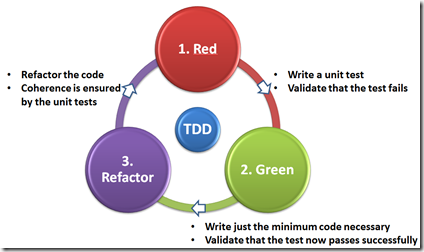
\includegraphics{programming/introduction/unit_test_tdd}

1. Definition 1 2

Test-driven development (TDD) is a software development process that relies on the repetition of a very short development cycle:

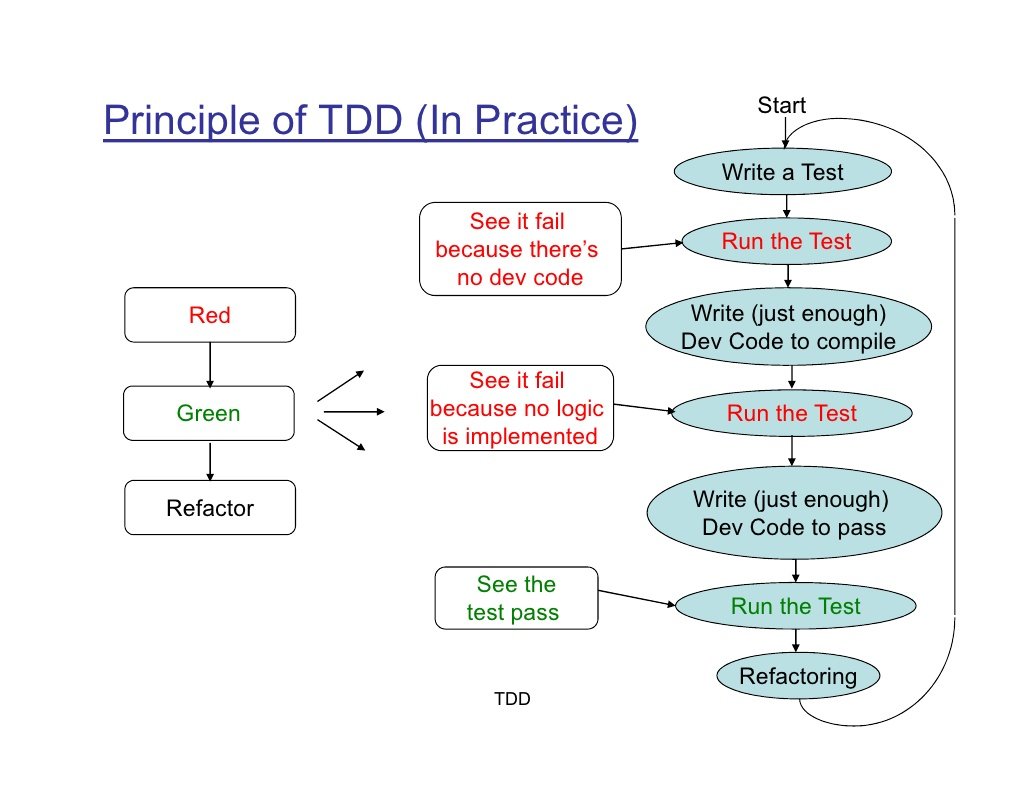
\includegraphics[width=\linewidth]{programming/introduction/tdd.jpg}

Step 1: First the developer writes an (initially failing) automated test case that defines a desired improvement or new function,

Step 2: Then produces the minimum amount of code to pass that test,

Step 3: Finally refactors the new code to acceptable standards.

Kent Beck, who is credited with having developed or 'rediscovered' the technique, stated in 2003 that TDD encourages simple designs and inspires confidence.

2. Principles 2

Kent Beck defines

Never with a single line of code unless you have a failing automated test.
Eliminate duplication
Red: (Automated test fail) Green (Automated test pass because dev code has been written) Refactor (Eliminate duplication, Clean the code)

3. Assertions & Assert Framework

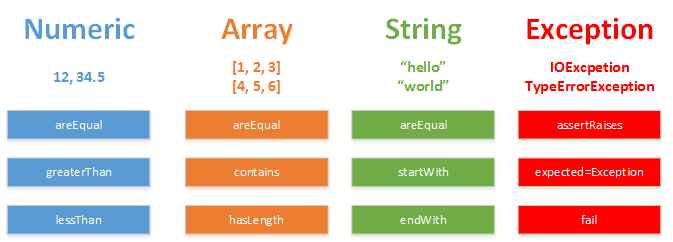
\includegraphics[width=\linewidth]{programming/introduction/tdd_assertion.png}

Assert that the expected results have occurred.
[code lang="java"] @Test public void test() { assertEquals(2, 1 + 1); } [/code]


4. Test Runners 3

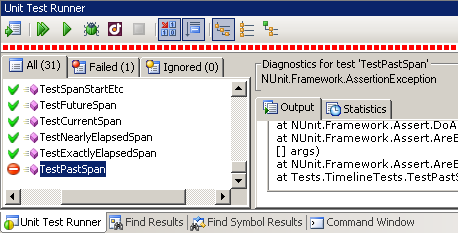
\includegraphics[width=\linewidth]{programming/introduction/tdd_test_runner.png}

When testing a large real-world web app there may be tens or hundreds of test cases, and we certainly don't want to run each one manually. In such as scenario we need to use a test runner to find and execute the tests for us, and in this article we'll explore just that.

A test runner provides the a good basis for a real testing framework. A test runner is designed to run tests, tag tests with attributes (annotations), and provide reporting and other features.

In general you break your tests up into 3 standard sections; setUp(), tests, and tearDown(), typical for a test runner setup.

The setUp() and tearDown() methods are run automatically for every test, and contain respectively:

The setup steps you need to take before running the test, such as unlocking the screen and killing open apps.
The cooldown steps you need to run after the test, such as closing the Marionette session.

5. Test Frameworks

Language	Test Frameworks
C++/VisualStudio	C++: Test
Web Service	rest-assured
Web UI	SeleniumHQ

\section{Logging}

Logging is the process of recording application actions and state to a secondary interface.


\includegraphics[width=\linewidth]{programming/introduction/logging}

Logging System

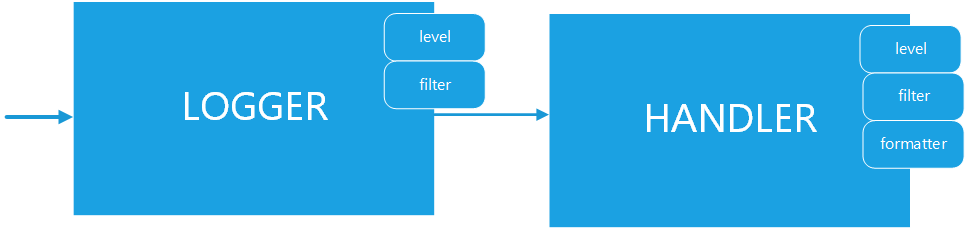
\includegraphics[width=\linewidth]{programming/introduction/logging_system}

Levels

Level	When it’s used
DEBUG	Detailed information, typically of interest only when diagnosing problems.
INFO	Confirmation that things are working as expected.
WARNING	An indication that something unexpected happened, or indicative of some problem in the near future (e.g. ‘disk space low’). The software is still working as expected.

ERROR

Due to a more serious problem, the software has not been able to perform some function.
CRITICAL	A serious error, indicating that the program itself may be unable to continue running.
Best Practices 2 4 5
Logging should always be considered when handling an exception but should never take the place of a real handler.
Keep all logging code in your production code. Have an ability to enable more/less detailed logging in production, preferably per subsystem and without restarting your program.
Make logs easy to parse by grep and by eye. Stick to several common fields at the beginning of each line. Identify time, severity, and subsystem in every line. Clearly formulate the message. Make every log message easy to map to its source code line.
If an error happens, try to collect and log as much information as possible. It may take long but it's OK because normal processing has failed anyway. Not having to wait when the same condition happens in production with a debugger attached is priceless.

\section{Lập trình hàm}

Functional
Without mutable variables, assignment, conditional

Advantages 1
Most functional languages provide a nice, protected environment, somewhat like JavaLanguage. It's good to be able to catch exceptions instead of having CoreDumps in stability-critical applications.
FP encourages safe ways of programming. I've never seen an OffByOne mistake in a functional program, for example... I've seen one. Adding two lengths to get an index but one of them was zero-indexed. Easy to discover though. -- AnonymousDonor
Functional programs tend to be much more terse than their ImperativeLanguage counterparts. Often this leads to enhanced programmer productivity.
FP encourages quick prototyping. As such, I think it is the best software design paradigm for ExtremeProgrammers... but what do I know.
FP is modular in the dimension of functionality, where ObjectOrientedProgramming is modular in the dimension of different components.
Generic routines (also provided by CeePlusPlus) with easy syntax. ParametricPolymorphism
The ability to have your cake and eat it. Imagine you have a complex OO system processing messages - every component might make state changes depending on the message and then forward the message to some objects it has links to. Wouldn't it be just too cool to be able to easily roll back every change if some object deep in the call hierarchy decided the message is flawed? How about having a history of different states?
Many housekeeping tasks made for you: deconstructing data structures (PatternMatching), storing variable bindings (LexicalScope with closures), strong typing (TypeInference), * GarbageCollection, storage allocation, whether to use boxed (pointer-to-value) or unboxed (value directly) representation...
Safe multithreading! Immutable data structures are not subject to data race conditions, and consequently don't have to be protected by locks. If you are always allocating new objects, rather than destructively manipulating existing ones, the locking can be hidden in the allocation and GarbageCollection system.

\section{Lập trình song song}

Paralell/Concurrency Programming
1. Callback Pattern 2
Callback functions are derived from a programming paradigm known as functional programming. At a fundamental level, functional programming specifies the use of functions as arguments. Functional programming was—and still is, though to a much lesser extent today—seen as an esoteric technique of specially trained, master programmers.

Fortunately, the techniques of functional programming have been elucidated so that mere mortals like you and me can understand and use them with ease. One of the chief techniques in functional programming happens to be callback functions. As you will read shortly, implementing callback functions is as easy as passing regular variables as arguments. This technique is so simple that I wonder why it is mostly covered in advanced JavaScript topics.

[code lang="javascript"] function getN(){ return 10; }

var n = getN();

function getAsyncN(callback){ setTimeout(function(){ callback(10); }, 1000); }

function afterGetAsyncN(result){ var n = 10; console.log(n); }

getAsyncN(afterGetAsyncN); [/code]

2. Promise Pattern 1 3
What is a promise?
The core idea behind promises is that a promise represents the result of an asynchronous operation.

A promise is in one of three different states:

pending - The initial state of a promise.
fulfilled - The state of a promise representing a successful operation.
rejected - The state of a promise representing a failed operation.
Once a promise is fulfilled or rejected, it is immutable (i.e. it can never change again).


\begin{lstlisting}[language=Javscript]
function aPromise(message){
  return new Promise(function(fulfill, reject){
    if(message == "success"){
      fulfill("it is a success Promise");
    } if(message == "fail"){
      reject("it is a fail Promise");
    }
  });
}
\end{lstlisting}

Usage:

\begin{lstlisting}[language=Javascript]
aPromise("success").then(function(successMessage){
  console.log(successMessage) }, function(failMessage){
  // it is a success Promise
  console.log(failMessage)
})
\end{lstlisting}

\begin{lstlisting}[language=Javascript]
aPromise("fail").then(function(successMessage){
  console.log(successMessage) }, function(failMessage){
  console.log(failMessage)
}) // it is a fail Promise
\end{lstlisting}

\section{IDE - Môi trường phát triển tích hợp}

An integrated development environment (IDE) is a software application that provides comprehensive facilities to computer programmers for software development. An IDE normally consists of a source code editor, build automation tools and a debugger. Most modern IDEs have intelligent code completion.

1. Navigation

Word Navigation Line Navigation File Navigation

2. Editing

Auto Complete Code Complete Multicursor Template (Snippets)

3. Formatting

Debugging
Custom Rendering for Object
  \part{Lập trình}

\chapter{Python}


\section{Cơ bản}

\textbf{Vấn đề với mảng}

\begin{item}
  \item Random Sampling \footnote{tham khảo [pytorch](http://pytorch.org/docs/master/torch.html?highlight=randn#torch.randn), [numpy](https://docs.scipy.org/doc/numpy-1.13.0/reference/routines.random.html))} - sinh ra một mảng ngẫu nhiên trong khoảng (0, 1), mảng ngẫu nhiên số nguyên trong khoảng (x, y), mảng ngẫu nhiên là permutation của số từ 1 đến n
\end{item}

\section{Quản lý gói với Anaconda}

\noindent Cài đặt package tại một branch của một project trên github

\begin{lstlisting}[language=bash]
  $ pip install git+https://github.com/tangentlabs/django-oscar-paypal.git@issue/34/oscar-0.6#egg=django-oscar-paypal
\end{lstlisting}

\noindent Trích xuất danh sách package

\begin{lstlisting}[language=bash]
 $ pip freeze > requirements.txt
\end{lstlisting}

\noindent \textbf{Chạy ipython trong environment anaconda}

\noindent Chạy đống lệnh này

\begin{lstlisting}[language=bash]
  conda install nb_conda
  source activate my_env
  python -m IPython kernelspec install-self --user
  ipython notebook
\end{lstlisting}

\noindent \textbf{Interactive programming với ipython}

\noindent Trích xuất ipython ra slide (không hiểu sao default `--to slides` không work nữa, lại phải thêm tham số `--reveal-prefix` [^1]

\begin{lstlisting}[language=bash]
jupyter nbconvert "file.ipynb"
  --to slides
  --reveal-prefix "https://cdnjs.cloudflare.com/ajax/libs/reveal.js/3.1.0"
\end{lstlisting}

**Tham khảo thêm**

* https://stackoverflow.com/questions/37085665/in-which-conda-environment-is-jupyter-executing
* https://github.com/jupyter/notebook/issues/541#issuecomment-146387578
* https://stackoverflow.com/a/20101940/772391

\noindent \textbf{python 3.4 hay 3.5}

Có lẽ 3.5 là lựa chọn tốt hơn (phải có của tensorflow, pytorch, hỗ trợ mock)

### Quản lý môi trường phát triển với conda

Chạy lệnh `remove` để xóa một môi trường

\begin{lstlisting}[language=bash]
conda remove --name flowers --all
\end{lstlisting}

\section{Test với python}

\textbf{Sử dụng những loại test nào?}

Hiện tại mình đang viết unittest với default class của python là Unittest. Thực ra toàn sử dụng `assertEqual` là chính!

Ngoài ra mình cũng đang sử dụng tox để chạy test trên nhiều phiên bản python (python 2.7, 3.5). Điều hay của tox là mình có thể thiết kế toàn bộ cài đặt project và các dependencies package trong file `tox.ini`

\textbf{Chạy test trên nhiều phiên bản python với tox}

Pycharm hỗ trợ debug tox (quá tuyệt!), chỉ với thao tác đơn giản là nhấn chuột phải vào file tox.ini của project.

\section{Xây dựng docs với readthedocs và sphinx}

\noindent \textbf{20/12/2017}: Tự nhiên hôm nay tất cả các class có khai báo kế thừa ở project languageflow không thể index được. Vãi thật. Làm thằng đệ không biết đâu mà build model.

Thử build lại chục lần, thay đổi file conf.py và package\_reference.rst chán chê không được. Giả thiết đầu tiên là do hai nguyên nhân (1) docstring ghi sai, (2) nội dung trong package\_reference.rst bị sai. Sửa chán chê cũng vẫn thể, thử checkout các commit của git. Không hoạt động!

Mất khoảng vài tiếng mới để ý thằng readthedocs có phần log cho từng build một. Lần mò vào build gần nhất và build (mình nhớ là) thành công cách đây 2 ngày

\noindent Log build gần nhất

\begin{lstlisting}[language=bash]
Running Sphinx v1.6.5
making output directory...
loading translations [en]... done
loading intersphinx inventory from https://docs.python.org/objects.inv...
intersphinx inventory has moved: https://docs.python.org/objects.inv -> https://docs.python.org/2/objects.inv
loading intersphinx inventory from http://docs.scipy.org/doc/numpy/objects.inv...
intersphinx inventory has moved: http://docs.scipy.org/doc/numpy/objects.inv -> https://docs.scipy.org/doc/numpy/objects.inv
building [mo]: targets for 0 po files that are out of date
building [readthedocsdirhtml]: targets for 8 source files that are out of date
updating environment: 8 added, 0 changed, 0 removed
reading sources... [ 12%] authors
reading sources... [ 25%] contributing
reading sources... [ 37%] history
reading sources... [ 50%] index
reading sources... [ 62%] installation
reading sources... [ 75%] package_reference
reading sources... [ 87%] readme
reading sources... [100%] usage

looking for now-outdated files... none found
pickling environment... done
checking consistency... done
preparing documents... done
writing output... [ 12%] authors
writing output... [ 25%] contributing
writing output... [ 37%] history
writing output... [ 50%] index
writing output... [ 62%] installation
writing output... [ 75%] package_reference
writing output... [ 87%] readme
writing output... [100%] usage
\end{lstlisting}

Log build hồi trước

\begin{lstlisting}[language=bash]
Running Sphinx v1.5.6
making output directory...
loading translations [en]... done
loading intersphinx inventory from https://docs.python.org/objects.inv...
intersphinx inventory has moved: https://docs.python.org/objects.inv -> https://docs.python.org/2/objects.inv
loading intersphinx inventory from http://docs.scipy.org/doc/numpy/objects.inv...
intersphinx inventory has moved: http://docs.scipy.org/doc/numpy/objects.inv -> https://docs.scipy.org/doc/numpy/objects.inv
building [mo]: targets for 0 po files that are out of date
building [readthedocs]: targets for 8 source files that are out of date
updating environment: 8 added, 0 changed, 0 removed
reading sources... [ 12%] authors
reading sources... [ 25%] contributing
reading sources... [ 37%] history
reading sources... [ 50%] index
reading sources... [ 62%] installation
reading sources... [ 75%] package_reference
reading sources... [ 87%] readme
reading sources... [100%] usage

/home/docs/checkouts/readthedocs.org/user_builds/languageflow/checkouts/develop/languageflow/transformer/count.py:docstring of languageflow.transformer.count.CountVectorizer:106: WARNING: Definition list ends without a blank line; unexpected unindent.
/home/docs/checkouts/readthedocs.org/user_builds/languageflow/checkouts/develop/languageflow/transformer/tfidf.py:docstring of languageflow.transformer.tfidf.TfidfVectorizer:113: WARNING: Definition list ends without a blank line; unexpected unindent.
../README.rst:7: WARNING: nonlocal image URI found: https://img.shields.io/badge/latest-1.1.6-brightgreen.svg
looking for now-outdated files... none found
pickling environment... done
checking consistency... done
preparing documents... done
writing output... [ 12%] authors
writing output... [ 25%] contributing
writing output... [ 37%] history
writing output... [ 50%] index
writing output... [ 62%] installation
writing output... [ 75%] package_reference
writing output... [ 87%] readme
writing output... [100%] usage
\end{lstlisting}

Đập vào mắt là sự khác biệt giữa documentation type

Lỗi

\begin{lstlisting}[language=bash]
building [readthedocsdirhtml]: targets for 8 source files that are out of date
\end{lstlisting}

Chạy

\begin{lstlisting}[language=bash]
building [readthedocs]: targets for 8 source files that are out of date
\end{lstlisting}

Hí ha hí hửng. Chắc trong cơn bất loạn sửa lại settings đây mà. Sửa lại nó trong phần Settings (Admin &gt; Settings &gt; Documentation type)

![](https://magizbox.files.wordpress.com/2017/10/screenshot-from-2017-12-20-09-54-23.png)

Khi chạy nó đã cho ra log đúng

\begin{lstlisting}[language=bash]
building [readthedocsdirhtml]: targets for 8 source files that are out of date
\end{lstlisting}

Nhưng vẫn lỗi. Vãi!!! Sau khoảng 20 phút tiếp tục bấn loạn, chửi bới readthedocs các kiểu. Thì để ý dòng này

Lỗi

\begin{lstlisting}[language=bash]
Running Sphinx v1.6.5
\end{lstlisting}


Chạy

\begin{lstlisting}[language=bash]
Running Sphinx v1.5.6
\end{lstlisting}

Ngay dòng đầu tiên mà không để ý, ngu thật. Aha, Hóa ra là thằng readthedocs nó tự động update phiên bản sphinx lên 1.6.5. Mình là mình chúa ghét thay đổi phiên bản (code đã mệt rồi, lại còn phải tương thích với nhiều phiên bản nữa thì ăn c** à). Đầu tiên search với Pycharm thấy dòng này trong `conf.py`

\begin{lstlisting}[language=bash]
# If your documentation needs a minimal Sphinx version, state it here.
# needs_sphinx = '1.0'
\end{lstlisting}

Đổi thành

\begin{lstlisting}[language=bash]
# If your documentation needs a minimal Sphinx version, state it here.
needs_sphinx = '1.5.6'
\end{lstlisting}

Vẫn vậy (holy sh*t). Thử sâu một tẹo (thực sự là rất nhiều tẹo). Thấy cái này trong trang Settings

![](https://magizbox.files.wordpress.com/2017/10/screenshot-from-2017-12-20-10-01-39.png)

Ờ há. Thằng đần này cho phép trỏ đường dẫn tới một file trong project để cấu hình dependency. Haha.
Tạo thêm một file `requirements` trong thư mục `docs` với nội dung

\begin{lstlisting}
sphinx==1.5.6
\end{lstlisting}


Sau đó cấu hình nó trên giao diện web của readthedocs

![](https://magizbox.files.wordpress.com/2017/10/screenshot-from-2017-12-20-10-04-49.png)

Build thử. Build thử thôi. Cảm giác đúng lắm rồi đấy. Và... nó chạy. Ahihi

![](https://magizbox.files.wordpress.com/2017/10/screenshot-from-2017-12-20-10-06-32.png)

\textbf{Kinh nghiệm}

* Khi không biết làm gì, hãy làm 3 việc. Đọc LOG. Phân tích LOG. Và cố gắng để LOG thay đổi theo ý mình.

PS: Trong quá trình này, cũng không thèm build thằng PDF với Epub nữa. Tiết kiệm được bao nhiêu thời gian.

\section{Pycharm Pycharm}

01/2018: Pycharm là trình duyệt ưa thích của mình trong suốt 3 năm vừa rồi.

Hôm nay tự nhiên lại gặp lỗi không tự nhận unittest, không resolve được package import bởi relative path. Vụ không tự nhận unittest sửa bằng cách xóa file .idea là xong. Còn vụ không resolve được package import bởi relative path thì vẫn chịu rồi. Nhìn code cứ đỏ lòm khó chịu thật.

\section{Vì sao lại code python?}

\textbf{01/11/2017}
Thích python vì nó quá đơn giản (và quá đẹp).

[^1]: https://github.com/jupyter/nbconvert/issues/91#issuecomment-283736634
  \chapter{Xác suất}

Phần này có thêm khảo \cite{Goodfellow-et-al-2016} và giáo trình xác suất thống kê của thạc sỹ Trần Thiện Khải, đại học Trà Vinh  \footnote{\href{http://www.ctec.tvu.edu.vn/ttkhai/xacsuatthongke_dh.htm}{http://www.ctec.tvu.edu.vn/ttkhai/xacsuatthongke\_dh.htm}}

\section{Các hàm phân phối thông dụng}

\textbf{17/01/2018} Lòng vòng thế nào hôm nay lại tìm được của bạn Đỗ Minh Hải \footnote{\href{https://dominhhai.github.io/vi/2017/10/prob-com-var}{https://dominhhai.github.io/vi/2017/10/prob-com-var}}, rất hay

\subsection{Biến rời rạc}

\subsubsection{Phân phối đều - Discrete Uniform distribution}

Là phân phối mà xác suất xuất hiện của các sự kiện là như nhau.
\newline
Biến ngẫu nhiên $X$ tuân theo phân phối đều rời rạc
$$X \sim \mathcal{U} (a, b)$$
với tham số $a, b \in \mathbb Z; a < b$ là khoảng giá trị của $X$, đặt $n = b-a+1$
\newline
Ta sẽ có:
\newline
\begin{tabular}{ | l | l | }
  \hline
  Định nghĩa & Giá trị \\
  \hline
  PMF & $p(x)$ | $\dfrac{1}{n}, \forall x \in [a,b]$ \\
  \hline
  CDF - $F(x;a,b)$ & $\dfrac{x-a+1}{n}, \forall x \in [a,b]$ \\
  \hline
  Kỳ vọng - $E[X]$ & $\dfrac{a+b}{2}$ \\
  \hline
  Phương sai - $Var(X)$ & $\dfrac{n^2-1}{12}$ \\
  \hline
\end{tabular}
\newline
Ví dụ: Lịch chạy của xe buýt tại một trạm xe buýt như sau: chiếc xe buýt đầu tiên trong ngày sẽ khởi hành từ trạm này vào lúc 7 giờ, cứ sau mỗi 15 phút sẽ có một xe khác đến trạm. Giả sử một hành khách đến trạm trong khoảng thời gian từ 7 giờ đến 7 giờ 30. Tìm xác suất để hành khách này chờ:

a) Ít hơn 5 phút.

b) Ít nhất 12 phút.

\textbf{Giải}

Gọi X là số phút sau 7 giờ mà hành khách đến trạm.

Ta có: $X \sim R[0;30]$.

a) Hành khách sẽ chờ ít hơn 5 phút nếu đến trạm giữa 7 giờ 10 và 7 giờ 15 hoặc giữa 7 giờ 25 và 7 giờ 30. Do đó xác suất cần tìm là:

$$P(0<X<15) + P(25<X<30)=\frac{5}{30} + \frac{5}{30}=\frac{1}{3}$$

b) Hành khách chờ ít nhất 12 phút nếu đến trạm giữa 7 giờ và 7 giờ 3 phút hoặc giữa 7 giờ 15 phút và 7 giờ 18 phút. Xác suất cần tìm là:

$$P(0<X<3) + P(15<X<18)=\frac{3}{30} + \frac{3}{30}=\frac{1}{5}$$

\subsubsection{Phân phối Béc-nu-li - Bernoulli distribution}

Như đã đề cập về phép thử Béc-nu-li rằng mọi phép thử của nó chỉ cho 2 kết quả duy nhất là $A$ với xác suất $p$ và $\bar A$ với xác suất $q=1-p$
Biến ngẫu nhiên $X$ tuân theo phân phối Béc-nu-li
$$X \sim B(p)$$
với tham số $p \in \mathbb{R}, 0 \leq p \leq 1$ là xác suất xuất hiện của $A$ tại mỗi phép thử
\newline
\begin{tabular}{ | l | l | l | }
  \hline
  Định nghĩa & & Giá trị \\
  \hline
  PMF & p(x) & $p(x)$ | $p^x (1-p)^{1-x}, x \in \{0, 1\} $ \\
  \hline
  CDF & $F(x;p)$  &
  \begin{cases}
    0 & \text{for } x < 0 \\
    1-p & \text{for } 0 \leq x < 1 \\
    1 & \text{for } x \geq 1
  \end{cases} \\
  \hline
  Kỳ vọng & $E[X]$ & $p$ \\
  \hline
  Phương sai & $Var(X)$ & $p(1-p)$ \\
  \hline
\end{tabular}
\newline

\textbf{Ví dụ}

Tham khảo thêm các thuật toán khác tại \cite{hai_2018}
  \part{Khoa học máy tính}

\chapter{Hệ điều hành}

\textbf{Những phần mềm không thể thiếu}

\begin{itemize}
  \item Adblock extension
  \item Trình duyệt Google Chrome (với các extensions Scihub, Mendeley Desktop, Adblock)
  \item Terminal (Oh-my-zsh)
  \item IDE Pycharm để code python
  \item Quản lý phiên bản code Git
  \item Bộ gõ ibus-unikey trong Ubuntu hoặc unikey (Windows) (Ctrl-Space để chuyển đổi ngôn ngữ)
  \item CUDA (lập trình trên GPU)
\end{itemize}

\textbf{Xem thông tin hệ thống}

Phiên bản `ubuntu 16.04`

\begin{lstlisting}
sudo apt-get install sysstat
\end{lstlisting}


Xem hoạt động (\%) của các core cpu

\begin{lstlisting}
mpstat -A
\end{lstlisting}


CPU của mình có bao nhiều core, bao nhiêu siblibngs

\begin{lstlisting}
cat /proc/cpuinfo

processor       : 23
vendor_id       : GenuineIntel
cpu family      : 6
model           : 62
model name      : Intel(R) Xeon(R) CPU E5-2430 v2 @ 2.50GHz
stepping        : 4
microcode       : 0x428
cpu MHz         : 1599.707
cache size      : 15360 KB
physical id     : 1
siblings        : 12
core id         : 5
cpu cores       : 6
apicid          : 43
initial apicid  : 43
fpu             : yes
fpu_exception   : yes
cpuid level     : 13
wp              : yes
flags           : fpu vme de pse tsc msr pae mce cx8 apic sep mtrr pge mca cmov pat pse36 clflush dts acpi mmx fxsr sse sse2 ss ht tm pbe syscall nx pdpe1gb rdtscp lm constant_tsc arch_perfmon pebs bts rep_good nopl xtopology nonstop_tsc aperfmperf eagerfpu pni pclmulqdq dtes64 monitor ds_cpl vmx smx est tm2 ssse3 cx16 xtpr pdcm pcid dca sse4_1 sse4_2 x2apic popcnt tsc_deadline_timer aes xsave avx f16c rdrand lahf_lm ida arat xsaveopt pln pts dtherm tpr_shadow vnmi flexpriority ept vpid fsgsbase smep erms
bogomips        : 5005.20
clflush size    : 64
cache_alignment : 64
address sizes   : 46 bits physical, 48 bits virtual
power management:
\end{lstlisting}

Kết quả cho thấy cpu của 6 core và 12 siblings

\textbf{Xem chương trình nào tốn ram}


\begin{lstlisting}
ps aux | awk '{print $2, $4, $11}' | sort -k2rn | head -n 20
\end{lstlisting}

\href{https://www.garron.me/en/go2linux/how-find-which-process-eating-ram-memory-linux.html}{https://www.garron.me/en/go2linux/how-find-which-process-eating-ram-memory-linux.html}


\chapter{Ubuntu}

\diary{27/12/2017: Lại dính lỗi không thể login. Lần này thì lại phải xóa bạn KDE đi. Kể cũng hơn buồn. Nhưng nhất quyết phải enable được tính năng Windows Spreading (hay đại loại thế). Hóa ra khi ubuntu bị lỗi không có lancher hay toolbar là do bạn unity plugin chưa được enable. Oài. Sao người hiền lành như mình suốt ngày bị mấy lỗi vớ vẩn thế không biết.}

\diary{20/11/2017: Hôm nay đen thật, dính lỗi login loop. Fix mãi mới được. Thôi cũng kệ. Cảm giác bạn KDE này đỡ bị lỗi ibus-unikey hơn bạn GNOME. Hôm nay cũng đổi bạn zsh theme. Chọn mãi chẳng được bạn nào ổn ổn, nhưng không thể chịu được kiểu suggest lỗi nữa rồi. Đôi khi thấy default vẫn là tốt nhất.}

\diary{21/11/2017: Sau một ngày trải nghiệm KDE, cảm giác giao diện mượt hơn GNOME. Khi overview windows với nhiều màn hình tốt và trực quan hơn. Đặc biệt là không bị lỗi ibus nữa. Đổi terminal cũng cảm giác ổn ổn. Không bị lỗi suggest nữa.}

\textbf{Chuyện terminal}

Terminal là một câu chuyện muôn thưở của bất kì ông coder nào thích customize, đẹp, tiện (và bug kinh hoàng). Hiện tại mình đang thấy combo này khá ổn Terminal (Ubuntu) (Color: Black on white, Build-in schemes: Tango) + zsh + oh-my-zsh (fishy-custom theme). Những features hay ho

\begin{itemize}
  \item Làm việc tốt trên cả Terminal (white background) và embedded terminal của Pycharm (black background)
  \item Hiển thị folder dạng ngắn (chỉ ký tự đầu tiên)
  \item Hiển thị brach của git ở bên phải
\end{itemize}


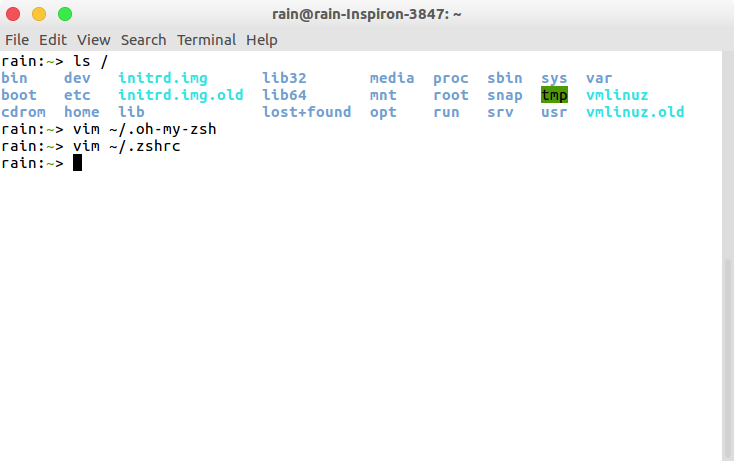
\includegraphics[width=10cm]{images/computer_science/ubuntu/terminal.png}

\textbf{Chuyện bộ gõ}

Làm sao để khởi động lại ibus, thỉnh thoảng lại chết bất đắc kì tử

\begin{lstlisting}
ibus-daemon &
ibus restart
\end{lstlisting}

\textbf{Chuyện lỗi login loop}

Phiên bản: `ubuntu 16.04`



\href{https://askubuntu.com/questions/389903/ibus-doesnt-seem-to-restart}{https://askubuntu.com/questions/389903/ibus-doesnt-seem-to-restart}

\textbf{Hot Corner và Workspace}

Cần cài đặt ngay \textbf{gnome-tweak-tool}

\begin{lstlisting}
sudo apt install gnome-tweak-tool
\end{lstlisting}

Cài đặt hot corner với

\href{https://askubuntu.com/questions/975348/how-to-get-all-hot-corner-in-ubuntu-17-10}{https://askubuntu.com/questions/975348/how-to-get-all-hot-corner-in-ubuntu-17-10}

Cài đặt Workspace
  \part{Khoa học dữ liệu}

%\chapter{Data Science with Python}

View online \href{http://magizbox.com/training/ml_data_python/site/}{http://magizbox.com/training/ml_data_python/site/}

The ability to analyze data with Python is critical in data science. Learn the basics, and move on to create stunning visualizations.

\section{Get Started}

Get Started with Ubuntu
Requirements

numpy, scipy
matplotlib
pandas
scikit-learn
ipython
Install pip

sudo apt-get install python-pip
Install numpy scipy

sudo apt-get install python-numpy python-scipy \
    python-matplotlib python-pandas python-sympy python-nose
Install scikit-learn

pip install jupyter ipython pip install -U scikit-learn

\section{Data Transformation}

DataFrame is a 2-dimensional labeled data structure with columns of potentially different types. You can think of it like a spreadsheet or SQL table, or a dict of Series objects. It is generally the most commonly used pandas object

Create data frame
Create new data frame from lists

\begin{lstlisting}[language=Python]
import pandas as pd
students = pd.DataFrame({
  "name" : ["Kate", "John", "Tom", "Mark"],
  "age" : [20, 21, 19, 18]
})
#       age  name
#    0   20  Kate
#    1   21  John
#    2   19   Tom
#    3   18  Mark
\end{lstlisting}

Load dataframe
Load dataframe from datasets


\begin{lstlisting}[language=Python]
import pandas as pd
from sklearn import datasets
iris_data = datasets.load_iris()
iris = pd.DataFrame(data=iris_data.data,
                    columns=iris_data.feature_names)
iris

\end{lstlisting}

Selection

Select by column index

\begin{lstlisting}[language=Python]
students.iloc[1:3, :]
#       age  name
#    1   21  John
#    2   19   Tom
\end{lstlisting}

Filter

\begin{lstlisting}[language=Python]
students = pd.DataFrame({
  'math' : [90, 80, 95, 50],
  'physic' : [20, 50, 95, 60]
})
#    math  physic
# 0    90      20
# 1    80      50
# 2    95      95
# 3    50      60

students[students['math'] > 85]
#    math  physic
# 0    90      20
# 2    95      95

students[students['math'] == students['physic']]
#    math  physic
# 2    95      95
\end{lstlisting}

Create new column

\begin{lstlisting}[language=Python]
students = pd.DataFrame({
  'name' : ["Kate", "John", "Tom", "Mark"],
  'age' : [20, 21, 19, 18]
})
students["birthyear"] = students.apply(
  lambda row: 2016 - row['age'], axis=1)
students["birthyear"] = 2016 - students["age"]
#       age  name  birthyear
#    0   20  Kate       1996
#    1   21  John       1995
#    2   19   Tom       1997
#    3   18  Mark       1998
\end{lstlisting}

Delete column

\begin{lstlisting}[language=Python]
students = pd.DataFrame({
  'name' : ["Kate", "John", "Tom", "Mark"],
  'age' : [20, 21, 19, 18]
})
students = students.drop('age', 1)
\end{lstlisting}

References

Wes McKinney, 10-minute tour of pandas: video, notebook

DataFrame, Intro to Data Structures

\section{Data Preperation}

Normalization

Example

\begin{lstlisting}[language=Python]
import numpy
from sklearn.preprocessing import normalize
matrix = numpy.arange(0,27,3).reshape(3,3).astype(numpy.float64)

# array([[  0.,   3.,   6.],
#   [  9.,  12.,  15.],
#   [ 18.,  21.,  24.]])

normed_matrix = normalize(matrix, axis=1, norm=‘l1’)

# [[ 0.          0.33333333  0.66666667]
# [ 0.25        0.33333333  0.41666667]
# [ 0.28571429  0.33333333  0.38095238]]
\end{lstlisting}

Label Encoder

Encode labels (categorical variables) with value between 0 and n_classes-1.

\begin{lstlisting}[language=Python]
import sklearn
le = sklearn.preprocessing.LabelEncoder()
le.fit([“paris”, “paris”, “tokyo”, “amsterdam”])
# LabelEncoder()
list(le.classes_)
# [‘amsterdam’, ‘paris’, ‘tokyo’]
le.transform([“tokyo”, “tokyo”, “paris”])
# array([2, 2, 1]...)
list(le.inverse_transform([2, 2, 1]))
# [‘tokyo’, ‘tokyo’, ‘paris’]
\end{lstlisting}

References

How to normalize a 2-dimensional numpy array in python less verbose?
sklearn.preprocessing.LabelEncoder

\section{Data IO}

This post shows how to import data to Python from numerous resources

CSV

Read a csv file from local or from a server

\begin{lstlisting}[language=Python]
import numpy as np
import pandas as pd
# read data
df = pd.read_csv(“data.csv”, header = 0)
# write data
df.to_csv(“data.csv”, header=1, index=False)
\end{lstlisting}

Excel

\begin{lstlisting}[language=Python]
import pandas as pd
# read data
df = pd.read_excel(“data.xls”)
# write data
df = pd.to_excel(“data.xls”, index=False)
\end{lstlisting}

Sqlite

\begin{lstlisting}[language=Python]
import sqlite3

DB_NAME = “db.sqlite3”
SELECT_QUERY = “SELECT page_id, type FROM service_page”
# connect to sqlite3
db_connector = sqlite3.connect(DB_NAME)
# excute query
cursor = db_connector.execute(SELECT_QUERY)
# return dataset
data_set = cursor.fetchall()
\end{lstlisting}

References

pandas.read_excel
pandas.read_sqlite
sqlite3.read_sqlite

\section{Numpy}

NumPy

Use the following import convention:

\begin{lstlisting}[language=Python]
import numpy as np
\end{lstlisting}

Creating Arrays

\begin{lstlisting}[language=Python]
a = np.array([1, 2, 3])
b = np.array([(1.5, 2, 3), (4, 5, 6)], dtype=float)
c = np.array([[(1.5, 2, 3), (4, 5, 6)], [(3, 2, 1), (4, 5, 6)]], dtype=float)
\end{lstlisting}

Initial Placeholders

\begin{lstlisting}[language=Python]
# Create an array of zeros
np.zeros((3, 4))
array([[ 0., 0., 0., 0.], [ 0., 0., 0., 0.], [ 0., 0., 0., 0.]])
\end{lstlisting}

# Create an array of ones

\begin{lstlisting}[language=Python]
np.ones((2, 3, 4), dtype=np.int16)

    array([[[1, 1, 1, 1],
            [1, 1, 1, 1],
            [1, 1, 1, 1]],

           [[1, 1, 1, 1],
            [1, 1, 1, 1],
            [1, 1, 1, 1]]], dtype=int16)

# Create an array of evenly spaced values (step value)
np.arange(10, 25, 5)
array([10, 15, 20])
# Create an array of evenly spaced values (number of samples)
np.linspace(0, 2, 9)
array([ 0. , 0.25, 0.5 , 0.75, 1. , 1.25, 1.5 , 1.75, 2. ])
# Create a constant array
np.full((2, 2), 7)
# array([[ 7., 7.], [ 7., 7.]])

# Create a 2x2 identity matirx
np.eye(2)
array([[ 1., 0.], [ 0., 1.]])
# Create an array with random values
np.random.random((2, 2))
array([[ 0.11121701, 0.12191919], [ 0.61608418, 0.91899253]])
# Create an empty array
np.empty((3, 2))
array([[ 0., 0.], [ 0., 0.], [ 0., 0.]])
\end{lstlisting}

IO

Saving & Loading On Disk

\begin{lstlisting}[language=Python]
a = np.array([(1, 2), (3, 4)])
b = np.array([(5, 6), (7, 8)])
np.save(‘my_array’, a)
np.savez(‘arrays’, a, b)
np.load(‘arrays.npz’)
\end{lstlisting}

Saving & Loading Text Files

\begin{lstlisting}[language=Python]
np.loadtxt(“myfile.txt”)
array([[ 1., 2., 3.], [ 2., 3., 4.]])
np.genfromtxt(“my_file.csv”, delimiter=”,“)
array([[ 1., 2., 3.], [ 4., 5., 6.]])
a = np.array([(1.5, 2, 3), (4, 5, 6)], dtype=float)
np.savetxt(“myarray.txt”, a, delimiter=” “)
\end{lstlisting}

Data Types

\begin{lstlisting}[language=Python]
# Signed 64-bit integer types
np.int64
# Stardard double-precision floating point
np.float32
# Complex numbers represented by 128 floats
np.complex
# Boolean type storing TRUE and FALSE values
np.bool
# Python object type
np.object
# Fixed-length string type
np.string_
# Fixed-length unicode type
np.unicode_
numpy.unicode_
\end{lstlisting}

Inspecting Your Array

\begin{lstlisting}[language=Python]
a = np.array([(1.5, 2, 3), (4, 5, 6)], dtype=float)
# array dimensions
a.shape
(2L, 3L)
# length of array
len(a)
2
# number of array dimensions
a.ndim
2
# number of array elements
a.size
6
# data type of array elements
a.dtype
dtype(‘float64’)
# name of data type
a.dtype.name
‘float64’
# convert an array to a different type
a.astype(int)
array([[1, 2, 3], [4, 5, 6]])
\end{lstlisting}

Asking For Help

\begin{lstlisting}[language=Python]
np.info(np.ndarray.dtype)
\end{lstlisting}

Data-type of the array’s elements. Parameters ————— None Returns ———- d : numpy dtype object See Also ———— numpy.dtype Examples ———— >>> x array([[0, 1], [2, 3]]) >>> x.dtype dtype(‘int32’) >>> type(x.dtype)

Array Mathmatics

Arithmetic Operations

\begin{lstlisting}[language=Python]
a = np.random.random((2, 2))
b = np.random.random((2, 2))
# subtraction
np.subtract(a, b)
a - b
array([[-0.04906355, 0.24579184], [ 0.45085259, 0.55266361]])
# addition
np.add(b, a)
b + a
array([[ 0.11861634, 1.28886181], [ 0.84371684, 1.37134298]])
# division
np.divide(a, b)
a / b
array([[ 0.41479504, 1.47128543], [ 3.29520803, 2.35013443]])
# multiplication
np.multiply(a, b)
a * b
array([[ 0.00291565, 0.40018778], [ 0.12714751, 0.39378613]])
# exponentiation
np.exp(b)
array([[ 1.08745483, 1.68461152], [ 1.21705271, 1.50582314]])
# square root
np.exp(b)
array([[ 1.08745483, 1.68461152], [ 1.21705271, 1.50582314]])
# sines of an array
np.sin(a)
array([[ 0.03476938, 0.69421365], [ 0.60302258, 0.82033885]])
# cosine of an array
np.cos(b)
array([[ 0.99648749, 0.86705545], [ 0.98076917, 0.91738383]])
# natural algorithm
np.log(a)
array([[-3.35881648, -0.26484246], [-0.43496903, -0.03873741]])
# dot product
a.dot(b)
np.dot(a, b)
array([[ 0.15364329, 0.33223443], [ 0.24323666, 0.73136775]])
\end{lstlisting}

Comparison

\begin{lstlisting}[language=Python]
a = np.random.random((2, 2))
a
array([[ 0.20271908, 0.83347777], [ 0.61463859, 0.47298106]])
b = np.random.random((2, 2))
b
array([[ 0.71492635, 0.48317927], [ 0.83547998, 0.67228618]])
# element-wise comparison
a == b
array([[False, False], [False, False]], dtype=bool)
# element-wise comparison
a < 2
array([[ True, True], [ True, True]], dtype=bool)
# array-wise comparison
np.array_equal(a, b)
False
\end{lstlisting}

Aggregate Functions

\begin{lstlisting}[language=Python]
a = np.random.random((3, 3))
a
array([[ 0.71770831, 0.895387 , 0.58199526], [ 0.32399079, 0.24146174, 0.59422847], [ 0.9976845 , 0.36588863, 0.67375734]])
# array-wise sum
a.sum()
5.392102026407013
# array-wise minimum value
a.min()
0.2414617386336485
# maximum value of an array row
a.max(axis=0)
array([ 0.9976845 , 0.895387 , 0.67375734])
# cumulative sum of the elements
a.cumsum(axis=1)
array([[ 0.71770831, 1.61309531, 2.19509057], [ 0.32399079, 0.56545253, 1.15968099], [ 0.9976845 , 1.36357313, 2.03733047]])
# mean
a.mean()
0.59912244737855702
# median
np.median(a)
0.59422846515666305
# correlation coefficient
np.corrcoef(a)
array([[ 1. , -0.93042812, -0.55310242], [-0.93042812, 1. , 0.20930732], [-0.55310242, 0.20930732, 1. ]])
# stardard deviation
np.std(a)
0.24142891382802531
Copy Arrays
a = np.random.random((3, 3))
a
array([[ 0.25274882, 0.19042929, 0.16823795], [ 0.39392342, 0.05954749, 0.8608243 ], [ 0.99375507, 0.92845989, 0.45681322]])
a.view()
array([[ 0.25274882, 0.19042929, 0.16823795], [ 0.39392342, 0.05954749, 0.8608243 ], [ 0.99375507, 0.92845989, 0.45681322]])
np.copy(a)
array([[ 0.25274882, 0.19042929, 0.16823795], [ 0.39392342, 0.05954749, 0.8608243 ], [ 0.99375507, 0.92845989, 0.45681322]])
h = a.copy()
h
array([[ 0.25274882, 0.19042929, 0.16823795], [ 0.39392342, 0.05954749, 0.8608243 ], [ 0.99375507, 0.92845989, 0.45681322]])
\end{lstlisting}

Sorting Arrays

\begin{lstlisting}[language=Python]
a = np.random.random((3, 3))
a
array([[ 0.11422752, 0.30046885, 0.15876115], [ 0.89595996, 0.47878824, 0.41827471], [ 0.69593773, 0.52119338, 0.33048738]])
a.sort()
a
array([[ 0.11422752, 0.15876115, 0.30046885], [ 0.41827471, 0.47878824, 0.89595996], [ 0.33048738, 0.52119338, 0.69593773]])
a.sort(axis=0)
a
array([[ 0.11422752, 0.15876115, 0.30046885], [ 0.33048738, 0.47878824, 0.69593773], [ 0.41827471, 0.52119338, 0.89595996]])
\end{lstlisting}

Subsetting, Slicing, Indexing

Subsettings

\begin{lstlisting}[language=Python]
a = np.random.random((3, 3))
a
array([[ 0.07989823, 0.4180309 , 0.83932547], [ 0.06318651, 0.20509151, 0.08262809], [ 0.64938826, 0.531026 , 0.38633983]])
# select the element at the 2nd index
a[2]
array([ 0.64938826, 0.531026 , 0.38633983])
# select the element at row 0 column 2
a[1][2]
a[1, 2]
0.08262808937797228
\end{lstlisting}

Slicing

\begin{lstlisting}[language=Python]
# select items at index 0 and 1
a[0:2]
array([[ 0.07989823, 0.4180309 , 0.83932547], [ 0.06318651, 0.20509151, 0.08262809]])
# select items at rớ 0 and 1 in column 1
a[0:2, 1]
array([ 0.4180309 , 0.20509151])
# select all items at row 0
a[1, ...]
a[1, ]
array([ 0.06318651, 0.20509151, 0.08262809])
# reversed array a
a[::-1]
array([[ 0.64938826, 0.531026 , 0.38633983], [ 0.06318651, 0.20509151, 0.08262809], [ 0.07989823, 0.4180309 , 0.83932547]])
\end{lstlisting}

Boolean indexing

\begin{lstlisting}[language=Python]
# select elements from a less than 0.5
a[a < 0.5]
array([ 0.07989823, 0.4180309 , 0.06318651, 0.20509151, 0.08262809, 0.38633983])
\end{lstlisting}

Fancy indexing

\begin{lstlisting}[language=Python]
# select elements (1,0), (0,1), (1, 2) and (0,0)
a[[1, 0, 1, 0], [0, 1, 2, 0]]
array([ 0.06318651, 0.4180309 , 0.08262809, 0.07989823])
# select a subset of the matrix’s rows and columns
a[[1, 0, 1, 0]][:, [0, 1, 2, 0]]
array([[ 0.06318651, 0.20509151, 0.08262809, 0.06318651], [ 0.07989823, 0.4180309 , 0.83932547, 0.07989823], [ 0.06318651, 0.20509151, 0.08262809, 0.06318651], [ 0.07989823, 0.4180309 , 0.83932547, 0.07989823]])
\end{lstlisting}

Array Manipulation

Transposing Array

\begin{lstlisting}[language=Python]
a = np.random.random((2, 3))
a
array([[ 0.57430709, 0.64401188, 0.12761183], [ 0.0726823 , 0.7951682 , 0.54114093]])
# permulate array dimensions
i = np.transpose(a)
i
array([[ 0.57430709, 0.0726823 ], [ 0.64401188, 0.7951682 ], [ 0.12761183, 0.54114093]])
# permulate array dimensions
i.T
array([[ 0.57430709, 0.64401188, 0.12761183], [ 0.0726823 , 0.7951682 , 0.54114093]])
\end{lstlisting}

Changing Array Shape

\begin{lstlisting}[language=Python]
# flatten the array
a.ravel()
array([ 0.57430709, 0.64401188, 0.12761183, 0.0726823 , 0.7951682 , 0.54114093])
# reshape, but don’t change data
a.reshape(3, -2)
array([[ 0.57430709, 0.64401188], [ 0.12761183, 0.0726823 ], [ 0.7951682 , 0.54114093]])
\end{lstlisting}

Adding/Removing Elements

\begin{lstlisting}[language=Python]
# return a new array with shape (2, 6)
a.resize(2, 3)
a
array([[ 0.57430709, 0.64401188, 0.12761183], [ 0.0726823 , 0.7951682 , 0.54114093]])
# append items to an array
h = np.random.random((2, 3))
print “h:”, h
g = np.random.random((2, 3))
print “g:”, g
np.append(h, g)
h: [[ 0.67964404 0.09256795 0.90630423] [ 0.52906489 0.51567697 0.95132012]] g: [[ 0.03126344 0.84908154 0.74228134] [ 0.40333143 0.28595213 0.68416838]] array([ 0.67964404, 0.09256795, 0.90630423, 0.52906489, 0.51567697, 0.95132012, 0.03126344, 0.84908154, 0.74228134, 0.40333143, 0.28595213, 0.68416838])
# insert items in an array
a = np.random.random((1, 3))
print “a:”, a
np.insert(a, 1, 0.5)
a: [[ 0.76135438 0.30331334 0.91866363]] array([ 0.76135438, 0.5 , 0.30331334, 0.91866363])
# delete items from an array
a = np.random.random((1, 3))
print “a:”, a
np.delete(a, [1])
a: [[ 0.1034073 0.93066432 0.49608264]] array([ 0.1034073 , 0.49608264])
\end{lstlisting}

Combining Arrays

\begin{lstlisting}[language=Python]
# concatenate arrays
a = np.random.random((1, 3))
print a
b = np.random.random((1, 3))
print b
np.concatenate((a, b), axis=0)
[[ 0.34496986 0.59502574 0.43416152]] [[ 0.98921435 0.68832237 0.44286195]] array([[ 0.34496986, 0.59502574, 0.43416152], [ 0.98921435, 0.68832237, 0.44286195]])
# stack arrays vertically (row-wise)
a = np.random.random((1, 3))
print a
b = np.random.random((2, 3))
print b
np.vstack((a, b)) #  equivalent to np.r_[a, b]
[[ 0.78793841 0.9923401 0.96372077]] [[ 0.75537083 0.09781391 0.25327948] [ 0.20607759 0.03763863 0.30818643]] array([[ 0.78793841, 0.9923401 , 0.96372077], [ 0.75537083, 0.09781391, 0.25327948], [ 0.20607759, 0.03763863, 0.30818643]])
# stack arrays horizontally (column-wise)
a = np.random.random((3, 1))
print a
b = np.random.random((3, 2))
print b
np.hstack((a, b))
[[ 0.33728008] [ 0.1091688 ] [ 0.68714517]] [[ 0.61421635 0.49316384] [ 0.19072731 0.04383904] [ 0.30587218 0.28743208]] array([[ 0.33728008, 0.61421635, 0.49316384], [ 0.1091688 , 0.19072731, 0.04383904], [ 0.68714517, 0.30587218, 0.28743208]])
# equivalent to np.hstack
np.column_stack((a, b))
array([[ 0.33728008, 0.61421635, 0.49316384], [ 0.1091688 , 0.19072731, 0.04383904], [ 0.68714517, 0.30587218, 0.28743208]])
# equivalent to np.hstack
np.c_[a, b]
array([[ 0.33728008, 0.61421635, 0.49316384], [ 0.1091688 , 0.19072731, 0.04383904], [ 0.68714517, 0.30587218, 0.28743208]])
\end{lstlisting}

Spliting Arrays

\begin{lstlisting}[language=Python]
a = np.random.random((3, 4))
print a
[[ 0.64277816 0.75935599 0.64927247 0.80253242] [ 0.87630664 0.19748931 0.51895547 0.83645583] [ 0.03132085 0.043291 0.10945252 0.31883126]]
# split the array horizontally at the 3rd index
np.split(a, 3)
[array([[ 0.64277816, 0.75935599, 0.64927247, 0.80253242]]), array([[ 0.87630664, 0.19748931, 0.51895547, 0.83645583]]), array([[ 0.03132085, 0.043291 , 0.10945252, 0.31883126]])]
# split the array vertically at the 3rd index
np.vsplit(a, 3)
[array([[ 0.64277816, 0.75935599, 0.64927247, 0.80253242]]), array([[ 0.87630664, 0.19748931, 0.51895547, 0.83645583]]), array([[ 0.03132085, 0.043291 , 0.10945252, 0.31883126]])]
\end{lstlisting}

Suggested Readings
www.datacamp.com. Python For Data Science Cheat Sheet: Numpy Basics

\section{Data Wrangling}

Learn about data wrangling with pandas

Tiny Data
A foundation for wrangling in pandas

Create DataFrames
Specify values for each column

\begin{lstlisting}[language=Python]
import pandas as pd

df = pd.DataFrame({
“a”: [4, 5, 6],
“b”: [7, 8, 9],
“c”: [10, 11, 12]
}, index=[1, 2, 3])
df
a b c

1 4 7 10

2 5 8 11

3 6 9 12
\end{lstlisting}

Specify values for each row

\begin{lstlisting}[language=Python]
df = pd.DataFrame(
[[4, 5, 6],
[7, 8, 9],
[10, 11, 12]],
index=[1, 2, 3],
columns=[“a”, “b”, “c”])
df
a b c
1 4 5 6
2 7 8 9
3 10 11 12
\end{lstlisting}

Create DataFrame with a MultiIndex

df = pd.DataFrame({
“a”: [4, 5, 6],
“b”: [7, 8, 9],
“c”: [10, 11, 12]
})
index = pd.MultiIndex.from_tuples(
[(‘d’, 1), (‘d’, 2), (‘e’, 2)],
names=[‘n’,‘v’])
df
a b c

0 4 7 10

1 5 8 11

2 6 9 12

Reshaping Data
melt
“Unpivots” a DataFrame from wide format to long format, optionally leaving identifier variables set.

import pandas as pd

df = pd.DataFrame({
“a”: [4, 5],
“b”: [7, 8],
“c”: [10, 11]
})
df
a b c

0 4 7 10

1 5 8 11

pd.melt(df)
variable value

0 a 4

1 a 5

2 b 7

3 b 8

4 c 10

5 c 11

pivot
Reshape data (produce a “pivot” table) based on column values. Uses unique values from index / columns to form axes of the resulting DataFrame.

df = pd.DataFrame({‘foo’: [‘one’,‘one’,‘one’,‘two’,‘two’,‘two’],
‘bar’: [‘A’, ‘B’, ‘C’, ‘A’, ‘B’, ‘C’],
‘baz’: [1, 2, 3, 4, 5, 6]})
df
bar baz foo

0 A 1 one

1 B 2 one

2 C 3 one

3 A 4 two

4 B 5 two

5 C 6 two

df.pivot(index=‘foo’, columns=‘bar’, values=‘baz’)
bar A B C

foo

one 1 2 3

two 4 5 6

df.pivot(index=‘foo’, columns=‘bar’)[‘baz’]
bar A B C

foo

one 1 2 3

two 4 5 6

concat
Append rows of DataFrames

df1 = pd.DataFrame([[‘a’, 1], [‘b’, 2]],
columns=[‘letter’, ‘number’])
df1
letter number

0 a 1

1 b 2

df2 = pd.DataFrame([[‘c’, 3], [‘d’, 4]],
columns=[‘letter’, ‘number’])
pd.concat([df1, df2])
letter number

0 a 1

1 b 2

0 c 3

1 d 4

Append columns of DataFrames

df1 = pd.DataFrame([[‘a’, 1], [‘b’, 2]],
columns=[‘letter’, ‘number’])
df1
letter number

0 a 1

1 b 2

df2 = pd.DataFrame([[‘bird’, ‘polly’], [‘monkey’, ‘george’]],
columns=[‘animal’, ‘name’])
df2
animal name

0 bird polly

1 monkey george

pd.concat([df1, df2], axis=1)
letter number animal name

0 a 1 bird polly

1 b 2 monkey george

sort
df = pd.DataFrame([[‘a’, 10, 1], [‘b’, 10, 5], [‘c’, 30, 3]],
columns=[‘name’, ‘age’, ‘score’])
df
name age score

0 a 10 1

1 b 10 5

2 c 30 3

order rows by values of a column (low to high)

df.sort_values(‘age’)
name age score

0 a 10 1

1 b 10 5

2 c 30 3

order rows by values of a column (high to low)

df.sort_values(‘age’, ascending=False)
name age score

2 c 30 3

0 a 10 1

1 b 10 5

order rows by values of two column

df.sort_values([‘age’, ‘score’], ascending=[False, False])
name age score

2 c 30 3

1 b 10 5

0 a 10 1

sort the index of a DataFrame

df.sort_index()
name age score

0 a 10 1

1 b 10 5

2 c 30 3

Reset index of DataFrame to row numbers, moving index to columns

df.reset_index()
index name age score

0 0 a 10 1

1 1 b 10 5

2 2 c 30 3

drop
drop columns from DataFrame

df.drop([‘age’, ‘score’], axis=1)
name
0	a
1	b
2	c

\section{Visualization}

An introduction about data visualization techniques using Matplotlib and Seaborn.

Gallery
 line graph
Line Graph

 bar graph
Bar Graph

 pie graph
Pie Graph

 sratter plot
Scatter Plot

References
Patterns: The Data Visualisation Catalogue




%\chapter{Trí tuệ nhân tạo}

View online \href{http://magizbox.com/training/ai/site/}{http://magizbox.com/training/ai/site/}

Artificial intelligence (AI) is the intelligence exhibited by machines or software. It is also the name of the academic field of study which studies how to create computers and computer software that are capable of intelligent behavior. Major AI researchers and textbooks define this field as "the study and design of intelligent agents", in which an intelligent agent is a system that perceives its environment and takes actions that maximize its chances of success. John McCarthy, who coined the term in 1955, defines it as "the science and engineering of making intelligent machines".

\section{Autonomous Agents}

limited ability to perceive its environment
process the environment and calculate an action
no global plan / leader
Vehicles

Action / Selection
Steering
Locomotion
Steering Behavior 1 2


Steering = Desired - Velocity

Seek
Flow Filed Following
Path Following
Group Steering
https://github.com/shiffman/The-Nature-of-Code-Examples/tree/master/chp06_agents\

Massive Battle: Coordinated Movement of Autonomous Agents ↩

Craig Reynolds, Steering Behaviors For Autonomous Characters ↩

\section{Cellular Automator}

https://www.youtube.com/watch?v=DKGodqDs9sA&index=1&list=PLRqwX-V7Uu6YrWXvEQFOGbCt6cX83Xunm

Cellular Automata

Grid of cell
Each cell has state, neighborhood
cell state at time t defined by a function of neighborhood states at time t-1
Elementary Cellular Automata

\section{Fractal}

L-System

\section{The Pac-Man project}

Today I found an interesting AI project - The Pac-Man

http://ai.berkeley.edu/images/pacman_game.gif

Here is the project overview

The Pac-Man projects were developed for UC Berkeley's introductory artificial intelligence course, CS 188. They apply an array of AI techniques to playing Pac-Man. However, these projects don't focus on building AI for video games. Instead, they teach foundational AI concepts, such as informed state-space search, probabilistic inference, and reinforcement learning. These concepts underly real-world application areas such as natural language processing, computer vision, and robotics. We designed these projects with three goals in mind. The projects allow students to visualize the results of the techniques they implement. They also contain code examples and clear directions, but do not force students to wade through undue amounts of scaffolding. Finally, Pac-Man provides a challenging problem environment that demands creative solutions; real-world AI problems are challenging, and Pac-Man is too. In our course, these projects have boosted enrollment, teaching reviews, and student engagement. The projects have been field-tested, refined, and debugged over multiple semesters at Berkeley. We are now happy to release them to other universities for educational use.
In the next part of this post, I will show my works on this project

Project 1: Search in Pacman

[caption id="" align="alignleft" width="231"]DFS[/caption]

[caption id="" align="alignleft" width="233"]BFS[/caption]
%\chapter{Học máy}

View online \href{http://magizbox.com/training/machinelearning/site/}{http://magizbox.com/training/machinelearning/site/}

\begin{itemize}
  \item Vấn đề với HMM và CRF?
  \item Học MLE và MAP?
\end{itemize}



Machine learning is a branch of science that deals with programming the systems in such a way that they automatically learn and improve with experience. Here, learning means recognizing and understanding the input data and making wise decisions based on the supplied data.

We can think of machine learning as approach to automate tasks like predictions or modelling. For example, consider an email spam filter system, instead of having programmers manually looking at the emails and coming up with spam rules. We can use a machine learning algorithm and feed it input data (emails) and it will automatically discover rules that are powerful enough to distinguish spam emails.

Machine learning is used in many application nowadays like spam detection in emails or movie recommendation systems that tells you movies that you might like based on your viewing history. The nice and powerful thing about machine learning is: It learns when it gets more data and hence it gets more and more powerful the more data we give them.

**Có bao nhiêu thuật toán Machine Learning?**

Có rất nhiều thuật toán Machine Learning, bài viết [Điểm qua các thuật toán Machine Learning hiện đại](https://ongxuanhong.wordpress.com/2015/10/22/diem-qua-cac-thuat-toan-machine-learning-hien-dai/) của Ông Xuân Hồng tổng hợp khá nhiều thuật toán. Theo đó, các thuật toán Machine Learning được chia thành các nhánh lớn như `regression`, `bayesian`, `regularization`, `decision tree`, `instance based`, `dimesionality reduction`, `clustering`, `deep learning`, `neural networks`, `associated rule`, `ensemble`... Ngoài ra thì còn có các cheatsheet của [sklearn](http://scikit-learn.org/stable/tutorial/machine_learning_map/index.html).

Việc biết nhiều thuật toán cũng giống như ra đường mà có nhiều lựa chọn về xe cộ. Tuy nhiên, quan trọng là có task để làm, sau đó thì cập nhật SOTA của task đó để biết các công cụ mới.

**Xây dựng model cần chú ý điều gì?**

Khi xây dựng một model cần chú ý đến vấn đề tối ưu hóa tham số (có thể sử dụng [GridSearchCV](sklearn.model_selection.GridSearchCV))

Bài phát biểu này có vẻ cũng rất hữu ích [PYCON UK 2017: Machine learning libraries you'd wish you'd known about](https://www.youtube.com/watch?v=nDF7_8FOhpI). Có đề cập đến

* [DistrictDataLabs/yellowbrick](https://github.com/DistrictDataLabs/yellowbrick) (giúp visualize model được train bởi sklearn)
* [marcotcr/lime](https://github.com/marcotcr/lime) (giúp inspect classifier)
* [TeamHG-Memex/eli5](https://github.com/TeamHG-Memex/eli5) (cũng giúp inspect classifier, hỗ trợ nhiều model như xgboost, crfsuite, đặc biệt có TextExplainer sử dụng thuật toán từ eli5)
* [rhiever/tpot](https://github.com/rhiever/tpot) (giúp tối ưu hóa pipeline)
* [dask/dask](https://github.com/dask/dask) (tính toán song song và lập lịch)

Ghi chú về các thuật toán trong xử lý ngôn ngữ tự nhiên tại [underthesea.flow/wiki](https://github.com/magizbox/underthesea.flow/wiki/Develop)

Framework để train, test hiện tại vẫn rất thoải mái sklearn. tensorboard cung cấp phần log cũng khá hay.

[Câu trả lời hay](https://www.quora.com/What-are-the-most-important-machine-learning-techniques-to-master-at-this-time/answer/Sean-McClure-3?srid=5O2u) cho câu hỏi [Những kỹ thuật machine learning nào quan trọng nhất để master?](https://www.quora.com/What-are-the-most-important-machine-learning-techniques-to-master-at-this-time), đặc biệt là dẫn đến bài [The State of ML and Data Science 2017](https://www.kaggle.com/surveys/2017) của Kaggle.

**Tài liệu học PGM**

[Playlist youtube](https://www.youtube.com/watch?v=WPSQfOkb1M8&amp;list=PL50E6E80E8525B59C) khóa học Probabilistic Graphical Models của cô Daphne Koller. Ngoài ra còn có một [tutorial](http://mensxmachina.org/files/software/demos/bayesnetdemo.html) dở hơi ở đâu về tạo Bayesian network

**[Chưa biết] Tại sao Logistic Regression lại là Linear Model?**

Trong quyển Deep Learning, chương 6, trang 165, tác giả có viết

```
Linear models, such as logistic regression and linear
regression, are appealing because they can be fit
efficiently and reliably, either in closed form or
with convex optimization
```

Mình tự hỏi tại sao logistic regression lại là linear, trong khi nó có sử dụng hàm logit (nonlinear)? Tìm hiểu hóa ra cũng có bạn hỏi giống mình trên [stats.stackexchange.com](https://stats.stackexchange.com/questions/93569/why-is-logistic-regression-a-linear-classifier). Ngoài câu trả lời trên stats.stackexchange, đọc một số cái khác [Generalized Linear Models, SPSS Statistics 22.0.0](https://www.ibm.com/support/knowledgecenter/en/SSLVMB_22.0.0/com.ibm.spss.statistics.help/spss/advanced/idh_idd_genlin_typeofmodel.htm)
và [6.1 - Introduction to Generalized Linear Models, Analysis of Discrete Data, Pennsylvania State University](https://onlinecourses.science.psu.edu/stat504/node/216) cũng vẫn chưa hiểu lắm.

Hiện tại chỉ hiểu là các lớp model này chỉ có thể hoạt động trên các tập linear separable, có lẽ do việc map input x, luôn có một liên kết linear $latex wx$, trước khi đưa vào hàm non-linear.

**Các tập dữ liệu thú vị**

*Iris dataset*: dữ liệu về hoa iris

Là một ví dụ cho bài toán phân loại

*Weather problem*: dữ liệu thời tiết. Có thể tìm được ở trong quyển Data Mining: Practical Machine Learning Tools and Techniques

Là một ví dụ cho bài toán cây quyết định

## Deep Learning

**Tài liệu Deep Learning**

Lang thang thế nào lại thấy trang này [My Reading List for Deep Learning!](https://www.microsoft.com/en-us/research/wp-content/uploads/2017/02/DL_Reading_List.pdf) của một anh ở Microsoft. Trong đó, (đương nhiên) có Deep Learning của thánh Yoshua Bengio, có một vụ hay nữa là bài review "Deep Learning" của mấy thánh Yann Lecun, Yoshua Bengio, Geoffrey Hinton trên tạp chí Nature. Ngoài ra còn có nhiều tài liệu hữu ích khác.

### Các layer trong deep learning [^2]

#### Sparse Layers

[**nn.Embedding**](http://pytorch.org/docs/master/nn.html#embedding) ([hướng dẫn](http://pytorch.org/tutorials/beginner/nlp/word_embeddings_tutorial.html))
★ grep code: [Shawn1993/cnn-text-classification-pytorch](https://github.com/Shawn1993/cnn-text-classification-pytorch/blob/master/model.py#L18)
Đóng vai trò như một lookup table, map một word với dense vector tương ứng

#### Convolution Layers

[**nn.Conv1d**](http://pytorch.org/docs/master/nn.html#conv1d), [**nn.Conv2d**](http://pytorch.org/docs/master/nn.html#conv2d), [**nn.Conv3d**](http://pytorch.org/docs/master/nn.html#conv3d) [^1]
★ grep code: [Shawn1993/cnn-text-classification-pytorch](https://github.com/Shawn1993/cnn-text-classification-pytorch/blob/master/model.py#L20-L24), [galsang/CNN-sentence-classification-pytorch](https://github.com/galsang/CNN-sentence-classification-pytorch/blob/master/model.py#L36-L38)

Các tham số trong Convolution Layer

* `kernel_size` (hay là filter size)

Đối với NLP, kernel_size thường bằng region_size * word_dim (đối với conv1d) hay (region_size, word_dim) đối với conv2d

<small>Quá trình tạo feature map đối với region size bằng 2</small>
![](https://media.giphy.com/media/l2QE2y1UQP7vIgiti/giphy.gif)

* `in_channels`, `out_channels` (là số lượng `feature maps`)

Kênh (channels) là các cách nhìn (view) khác nhau đối với dữ liệu. Ví dụ, trong ảnh thường có 3 kênh RGB (red, green, blue), có thể áp dụng convolution giữa các kênh. Với văn bản cũng có thể có các kênh khác nhau, như khi có các kênh sử dụng các word embedding khác nhau (word2vec, GloVe), hoặc cùng một câu nhưng biểu diễn ở các ngôn ngữ khác nhau.

* `stride`

Định nghĩa bước nhảy của filter.

![](http://d3kbpzbmcynnmx.cloudfront.net/wp-content/uploads/2015/11/Screen-Shot-2015-11-05-at-10.18.08-AM-1024x251.png)

Hình minh họa sự khác biệt giữa các feature map đối với stride=1 và stride=2. Feature map đối với stride = 1 có kích thước là 5, feature map đối với stride = 3 có kích thước là 3. Stride càng lớn thì kích thước của feature map càng nhỏ.

Trong bài báo của Kim 2014, `stride = 1` đối với `nn.conv2d` và `stride = word_dim` đối với `nn.conv1d`

Toàn bộ tham số của mạng CNN trong bài báo Kim 2014,

![](http://d3kbpzbmcynnmx.cloudfront.net/wp-content/uploads/2015/11/Screen-Shot-2015-11-06-at-8.03.47-AM.png)

| Description | Values |
|---------------------|-----------------|
| input word vectors | Google word2vec |
| filter region size | (3, 4, 5)       |
| feature maps | 100 |
| activation function | ReLU |
| pooling | 1-max pooling |
| dropout rate | 0.5 |
| $latex l&amp;s=2$2 norm constraint | 3 |

Đọc thêm:

* [Lecture 13: Convolutional Neural Networks (for NLP). CS224n-2017](http://web.stanford.edu/class/cs224n/lectures/cs224n-2017-lecture13-CNNs.pdf)
* [DeepNLP-models-Pytorch - 8. Convolutional Neural Networks](https://nbviewer.jupyter.org/github/DSKSD/DeepNLP-models-Pytorch/blob/master/notebooks/08.CNN-for-Text-Classification.ipynb)
* [A Sensitivity Analysis of (and Practitioners’ Guide to) Convolutional Neural Networks for Sentence Classification. Zhang 2015](https://arxiv.org/pdf/1510.03820.pdf)

**BTS**

22/11/2017 - Phải nói quyển này hơi nặng so với mình. Nhưng thôi cứ cố gắng vậy.
24/11/2017 - Từ hôm nay, mỗi ngày sẽ ghi chú một phần (rất rất nhỏ) về Deep Learning [tại đây](https://docs.google.com/document/d/1KxDrw5s6uYHNLda7t0rhp0RM_TlUGxydQ-Qi1JOPFr8/edit?usp=sharing)

[^1]: [Understanding Convolutional Neural Networks for NLP](http://www.wildml.com/2015/11/understanding-convolutional-neural-networks-for-nlp)
[^2]: [http://pytorch.org/docs/master/nn.html](http://pytorch.org/docs/master/nn.html)

\section{Machine Learning Process}

The good life is a process, not a state of being. It is a direction not a destination.

Carl Rogers


I searched a framework fit for every data mining task, I found a good one from an article of Oracle.

And here is my summary. The data mining process has 4 steps:

Step 1. Problem Definition

This initial phase of a data mining project focuses on understanding the project objectives and requirements. Once you have specified the project from a business perspective, you can formulate it as a data mining problem and develop a preliminary implementation plan.

Step 2. Data Gathering & Preparation

The data understanding phase involves data collection and exploration. As you take a closer look at the data, you can determine how well it addresses the business problem. You might decide to remove some of the data or add additional data. This is also the time to identify data quality problems and to scan for patterns in the data.

Data Access
Data Sampling

Data Transformation

Data in the real world is dirty [3]. They are often incomplete (lacking attribute values, lacking certain attributes of interest, or containing only aggregate data), noisy (containing errors or outliers),‰ inconsistent (containing discrepancies in codes or names). Step 3. Model Building In this phase, you select and apply various modeling techniques and calibrate the parameters to optimal values. If the algorithm requires data transformations, you will need to step back to the previous phase to implement them

Create Model
Test Model

Evaluate & Interpret Model

Some important questions [2]:

Is at least one of predictors useful in predicting the response? (F-statistics)
Do all the predictors help to explain Y, or is only a subset of the predictors useful? (all subsets or best subsets)
How well does the model fit the data?
Given a set of predictor values, what response value should we predict, and how accurate is our prediction?
Step 4. Knowledge Deployment Knowledge deployment is the use of data mining within a target environment. In the deployment phase, insight and actionable information can be derived from data.
Model Apply
Custom Reports
External Applications
References
The Data Mining Process, Oracle
Trevor Hastie and Rob Tibshirani, Model Selection and Qualitative Predictors, URL:https://www.youtube.com/watch?v=3T6RXmIHbJ4
Nguyen Hung Son, Data cleaning and Data preprocessing, URL:http://www.mimuw.edu.pl/~son/datamining/DM/4-preprocess.pdf

\subsection{Problem Definition}

This initial phase of a data mining project focuses on understanding the project objectives and requirements. Once you have specified the project from a business perspective, you can formulate it as a data mining problem and develop a preliminary implementation plan.

For example, your business problem might be: "How can I sell more of my product to customers?" You might translate this into a data mining problem such as: "Which customers are most likely to purchase the product?" A model that predicts who is most likely to purchase the product must be built on data that describes the customers who have purchased the product in the past. Before building the model, you must assemble the data that is likely to contain relationships between customers who have purchased the product and customers who have not purchased the product. Customer attributes might include age, number of children, years of residence, owners/renters, and so on.

\subsection{Data Gathering}

The data understanding phase involves data collection and exploration. As you take a closer look at the data, you can determine how well it addresses the business problem. You might decide to remove some of the data or add additional data. This is also the time to identify data quality problems and to scan for patterns in the data.

The data preparation phase covers all the tasks involved in creating the case table you will use to build the model. Data preparation tasks are likely to be performed multiple times, and not in any prescribed order. Tasks include table, case, and attribute selection as well as data cleansing and transformation. For example, you might transform a DATE_OF_BIRTH column to AGE; you might insert the average income in cases where the INCOME column is null.

Additionally you might add new computed attributes in an effort to tease information closer to the surface of the data. For example, rather than using the purchase amount, you might create a new attribute: "Number of Times Amount Purchase Exceeds $500 in a 12 month time period." Customers who frequently make large purchases may also be related to customers who respond or don't respond to an offer.

Thoughtful data preparation can significantly improve the information that can be discovered through data mining.

Data Sources
Open Data

wikipedia dumps: https://dumps.wikimedia.org/other/pagecounts-raw/

\subsection{Data Preprocessing}

The quality of the data and the amount of useful information it contains affect greatly how well an algorithm can learn. Hence, it is important to preprocess the dataset before using it. The most common preprocessing steps are: removing missing values, converting categorical data into shape suitable for machine learning algorithm and feature scaling.

Missing Data
Sometimes the samples in the dataset are missing some values and we want to deal with these missing values before passing it to the machine learning algorithm. There are a number of strategies we can follow

Remove samples with missing values: This approach is by far the most convenient but we may end up removing too many samples and by that we would be losing valuable information that can help the machine learning algorithm.
Imputing missing values: Instead of removing the entire sample we use interpolation to estimate the missing values. For example, we could substitute a missing value by the mean of the entire column.
Categorical Data
In general, features can be numerical (e.g. price, length, width, etc…) or categorical (e.g. color, size, etc..). Categorical features are further split into nominal and ordinal features.

Ordinal features can be sorted and ordered. For example, size (small, medium, large), we can order these sizes large > medium > small. While nominal features do not have an order for example, color, it doesn’t make any sense to say that red is larger than blue.

Most machine learning algorithm require that you convert categorical features into numerical values. One solution would to assign each value a different number starting from zero. (e.g. small à 0 ,medium à 1 ,large à 2)

This works well for ordinal features but might cause problems with nominal features (e.g. blue à 0, white à 1, yellow à 2) because even though colors are not ordered the learning algorithm will assume that white is larger than blue and yellow is larger than white and this is not correct.

To get around this problem is to use one-hot encoding, the idea is to create a new feature for each unique value of the nominal feature.


In the above example, we converted the color feature into three new features Red, Green, Blue and we used binary values to indicate the color. For example, a sample with “Red” color is now encoded as (Red=1, Green=0, Blue=0)

Feature Scaling
Why have we do Feature Scaling?

We have to predict the house prices base on 2 features:

House sizes (feet2)
Number of bedrooms in the house
And we relized that house sizes are about 1000 times the number of bedrooms. When features differ by orders of magnitude, first performing feature scaling can make gradient descent converge much more quickly.

Perform Feature Scaling

Subtract the mean value (the average value) of each feature from the dataset.
After subtracting the mean, additionally scale (divide) the feature values by their respective "standard deviations."
Function: x′=x−x¯σx′=x−x¯σ where xx is the original feature vector, x¯x¯ is the mean of that feature vector, and σσ is its standard deviation.
Feature Scaling Function implementation in Octave

function [X_norm, mu, sigma] = featureNormalize(X)
X_norm = X;
mu = zeros(1, size(X, 2)); % storing the mean value in mu
sigma = zeros(1, size(X, 2)); % storing the standard deviation in sigma

for i = 1:length(mu),
mu(i) = mean(X(:,i));
end;

for i = 1:length(sigma),
sigma(i) = std(X(:,i));
end;

X_norm = (X .- mu)./sigma;
end
Related Reading
Introduction to Machine Learning

\subsection{Model Building}

In this phase, you select and apply various modeling techniques and calibrate the parameters to optimal values. If the algorithm requires data transformations, you will need to step back to the previous phase to implement them

Create Model
Test Model
Evaluate & Interpret Model
Some important questions

Is at least one of predictors useful in predicting the response? (F-statistics)
Do all the predictors help to explain Y, or is only a subset of the predictors useful? (all subsets or best subsets)
How well does the model fit the data?
Given a set of predictor values, what response value should we predict, and how accurate is our prediction?
Create Model
First thing first, start with simple and fast model, then you known how difficult the problem is.

One import thing is create a well pipeline for your experiments, it is very helpful in turning features, model selection, save your experiment and write reports.

Feature Selections
After train model, some model will give active features (such as CRF), it is clue for you to feature selection. If amount active features is too small compared to amount features, it is the problem. In this case the better way to enhance is try reduce amount of features and see how well this set fit data. Keep in mind the more number of features is, the complex model is, and it will make your model over fitting.
Storing the model
Number of active features: 5566 (35383)
Number of active attributes: 4343 (20722)
example after training crf model with python-crfsuite
Test Model
This phase determines how well the model fit data. See Evaluation for details.

What to do next
In an interview Andrew Ng said about building machine learning model

"I often make an analogy to building a rocket ship. A rocket ship is a giant engine together with a ton of fuel. Both need to be really big. If you have a lot of fuel and a tiny engine, you won’t get off the ground. If you have a huge engine and a tiny amount of fuel, you can lift up, but you probably won’t make it to orbit. So you need a big engine and a lot of fuel.

The reason that machine learning is really taking off now is that we finally have the tools to build the big rocket engine — that is giant computers, that’s our rocket engine. And the fuel is the data. We finally are getting the data that we need."

We need both big rocket engine and data to make our model works.

Related Reading
Inside The Mind That Built Google Brain: On Life, Creativity, And Failure, huffingtonpost.com

\subsection{Evaluation}

Training vs Test Data
We typically split the input data into learning and testing datasets. The then run the machine learning algorithm on the learning dataset to generate the prediction model. Later, we use the test dataset to evaluate our model.


It is important that the test data is separate from the one used in training otherwise we will be kind of cheating because may for example the generated model memorizes the data and hence if the test data is also part of the training data then our evaluation scores of the model will be higher than they actually are.

The data is usually split 75% training and 25% data or 2/3 training and 1/3 testing. It is important to note that: the smaller the training set the more challenging it is for the algorithm to discover the rules.

In addition, when splitting the dataset, you need to maintaining class proportions and population statistics otherwise we will have some classes that are under represented in the training dataset and over represented in the test dataset.

For example, you may have 100 sample and a total of 80 samples are labeled with Class-A and the remaining 20 instances are labeled with Class-B. you want to make sure when splitting the data that you maintain this representation.

One way to avoid this problem and to make sure that all classes are represented in both training and testing datasets is stratification. It is the process of rearranging the data as to ensure each set is a good representative of the whole. In our previous example, (80/20 samples), it is best to arrange the data such that in every set, each class comprises around 80:20 ratios of the two classes.

Cross Validation
A crucial step when building our machine learning model is to estimate its performance on that that the model hadn't seen before. We want to make sure that the model generalizes well to new unseen data.

One case, the machine learning algorithm has different parameters and we want to tune these parameters to achieve the best performance. (Note: the parameters of the machine learning algorithm are called hyperparameters). Another case, sometimes we want to try out different algorithms and choose the best performing one. Below are some of the techniques used.

Holdout Method
We simply split the data into training and testing datasets. We train the algorithm on the training dataset to generate a model. In order, to evaluate different algorithms we use the testing data to evaluate each algorithm.

However, if we reuse the same test dataset over and over again during algorithm selection, the test data has now come part of the training data. Hence, when we use the test data for the final evaluation the generated model is biased towards the test data and the performance score is optimistic.

Holdout Validation
As before, we split the data into training and testing dataset. Then, the training data is further split into training and validation sets.

The training data is used to train different models. Then the validation data is used to compute performance of each of them and we select the best one. Finally, the model is then used for the test set to evaluate performance. The next figure illustrates this idea.


However, because we use the validation set multiple times, Holdout validation is sensitive to how we partition the data and that is what K-fold cross validation tries to solve.

K-fold cross validation
Initially, we split the data into training and testing dataset. Furthermore, the training dataset is split into K chunks.

Suppose we will use 5-fold cross validation, the training data set is split into 5 chunks and the training phase will take place over 5 iterations. In each iteration we use one chunk as the validation dataset while the rest of the chunk are grouped together to form the training dataset.

This is very similar to Holdout validation except in each iteration the validation data is different and this removed the bias. Each iteration generates a score and the final score is the average score of all iteration. As before we select the best model and use the test data for the final performance evaluation.

Related Readings

Introduction to Machine Learning

\section{Types of Machine Learning}

There are three different types of machine learning: supervised, unsupervised and reinforcement learning. 4

Supervised Learning
The goal of supervised learning is to learn a model from labelled training data that allows us to make predictions about future data. For supervised machine learning to work we need to feed the algorithm two things: the input data and our knowledge about it labels).

The spam filter example mentioned earlier is a good example of supervised learning; we have a bunch of emails (data) and we know whether each email is spam or not (labels).


Supervised learning can be divided into two subcategories:

Classification: It is used to predict categories or class labels based on past observations i.e. we have discrete variable you want to distinguish into discrete categorical outcome. For example, in the email spam filter system the output is discrete "spam" or "not spam".
Regression: It is used to predict a continuous outcome. For example, to determine the price of houses and how it is affected by the number of rooms in that house. The input data is the house features (no. of rooms, location, size in square feet,) and the output is the price (the continuous outcome).
Unsupervised Learning
The goal of unsupervised learning is to discover hidden structure or patterns in unlabeled data and it can be divided into two subcategories

Clustering: It is used to organize information into meaningful clusters (subgroups) without having prior knowledge of their meaning. For example, the figure below shows how we can use clustering to organize unlabeled data into groups based on their features.


Dimensionality Reduction (Compression): It is used to reduce a higher dimension data into a lower dimension ones. To put it more clearly consider this example. A telescope has terabytes of data and not all of these data can be stored and so we can use dimensionality reduction to extract the most informative features of these data to be stored. Dimensionality reduction is also a good candidate to visualize data because if you have data in higher dimensions you can compress it to 2D or 3D to easily plot and visualize it.

Reinforcement Learning

The goal of reinforcement learning is to develop a system that improves its performance based on the interaction with a dynamic environment and there is a delayed feedback that act as a reward. i.e. reinforcement learning is learning by doing with a delayed reward. A classic example of reinforcement learning is a chess game, the computer decided a series of moves and the reward is the "win" or "lose" at the end the game.

You might think that this is similar to supervised learning where the reward is basically a label for the data but the core difference is this feedback/reward is not the truth but it is a measure of how well the action to achieving a certain goal.

Microsoft Azure Machine Learning 1


Machine Learning Cheat Sheet for scikit-learn 2


DLib C++ Library - Machine Learning Guide 3


Challenges
Very much features (> 100)
Very much data (> 1e9 items)
Text Data, Images, Videos
Training Times
Accuracy, Over Fitting
Machine learning algorithm cheat sheet for Microsoft Azure Machine Learning Studio ↩

Machine Learning Cheat Sheet (for scikit-learn) ↩

DLib C++ Library - Machine Learning Guide ↩

Introduction to Machine Learning ↩

\section{How to learn a ML Algorithm?}

1. Motivation

Each algorithm have its own motivation. It may a simple example to see how it work

2. Problem Definition

Where can we apply this algorithm? How did it work in real world applications

3. Mathematics Representation

Problem Equations, notations

We will discuss about mathematics representation of algorithm, notations we use for problem

4. Algorithm

We will discuss how to solve this mathematics problems

5. Examples

We will apply algorithm with a few examples (1-2 dimension is highly recommended, because we will plot these data and model easily)

In this section, we can see how well (bad) algorithm works with these data

6. Implementation Notice

We will give some notes about implement this algorithm to real world problems. What case we want to apply this algorithm? What case we don't?

7. Quiz

One way to rethink about problem is doing quiz.

8. Exercise


\section{Linear Regression}

\index{hồi quy tuyến tính|see {linear regression}}
\definition{linear regression}{
Hồi quy tuyến tính, là thuật toán machine learning cơ bản nhất, áp dụng trên dữ liệu số
}

\noindent\textbf{In-Out}

\begin{itemize}
  \item Đầu vào: Continuous
  \item Đầu ra: Continuous
\end{itemize}

\noindent \textbf{When to use}

\begin{itemize}
  \item Econometric Modeling
  \item Marketing Mix Model
  \item Customer Lifetime Value
\end{itemize}

\noindent \textbf{Examples}

\noindent Ex. Linear Regression with Boston Dataset

\begin{lstlisting}[language=Python]
__author__ = 'rain'

from sklearn.datasets import load_boston
from sklearn.cross_validation import train_test_split
from sklearn.linear_model import LinearRegression, Ridge
boston = load_boston()
data = boston['data']
X, y = data[:, :-1], data[:, -1]
X_train, X_test, y_train, y_test =
train_test_split(X, y, test_size=0.3)
print boston['DESCR']
clf_linear = LinearRegression()
clf_linear.fit(X_train, y_train)
linear_score = clf_linear.score(X_test, y_test)
#-> 0.671
print(clf_linear.coef_)
print(clf_linear.intercept_)

clf_ridge = Ridge(alpha=1.0)
clf_ridge.fit(X_train, y_train)
# 0.674
ridge_score = clf_ridge.score(X_test, y_test)

print y_test
print clf_linear.predict(X_test)
print clf_ridge.predict(X_test)
\end{lstlisting}

\section{Logistic Regression}

\index{hồi quy logistic|see {logistic regression}}
\definition{logistic regression}{
Mô hình đơn giản nhất của việc phân lớp, dựa vào hàm logistic
}

\noindent\textbf{In-Out}

\begin{itemize}
  \item Đầu vào: continuos
  \item Đầu ra: True/False
\end{itemize}

\noindent\textbf{Hyposthesis Representation}

$$h_\theta (x) = g(\theta^Tx) \textnormal{ trong đó } g(z)=\frac{1}{1+e^{−z}}$$

$g(z)$ là hàm sigmoid hay hàm logistic

$h_\theta (x)$ estimated probability of y=1  given $x$

\text{In spam detection problem, hθ(x)=0.7 means it's 70\% chance this email is spam.}


\noindent\textbf{Decision Boundary}

Logistic Regression

\noindent\textbf{Cost Function}

cost(hθ(x),y)=−ylog(hθ(x))−(1−y)log(1−hθ(x))
cost(hθ(x),y)=−ylog(hθ(x))−(1−y)log(1−hθ(x))

Loss Function

$$J(θ)=1m∑i=1mcost(hθ(x(i)),y(i))=−1m∑i=1my(i)loghθ(x(i))+(1−y(i))log(1−hθ(x(i)))$$

\noindent\textbf{Gradient Descent}

Gradient

$$∂J(θ)∂θj=1m∑i=1m(hθ(x(i))−y(i))x(i)j$$

\noindent\textbf{Predict}

$$p(θ,X)=hθ(X)≥0.5$$

\noindent\textbf{Regularization}

6.1 Feature Mapping

Cost Function

mapFeature(x)=⎡⎣⎢⎢⎢⎢⎢⎢⎢⎢⎢⎢⎢⎢⎢⎢⎢⎢⎢⎢⎢⎢1x1x2x21x1x2x22x31⋯x1x52x62⎤⎦⎥⎥⎥⎥⎥⎥⎥⎥⎥⎥⎥⎥⎥⎥⎥⎥⎥⎥⎥⎥
mapFeature(x)=[1x1x2x12x1x2x22x13⋯x1x25x26]

6.2 Cost Function and Gradient
Cost Function
J(θ)=1m∑i=1m[−y(i)log(hθ(x(i)))−(1−y(i))log(1−hθ(x(i)))]+λ2m∑j=1nθ2j
J(θ)=1m∑i=1m[−y(i)log(hθ(x(i)))−(1−y(i))log(1−hθ(x(i)))]+λ2m∑j=1nθj2
Gradient

∂J(θ)∂θj=1m∑mi=1(hθ(x(i))−y(i))x(i)j∂J(θ)∂θj=1m∑i=1m(hθ(x(i))−y(i))xj(i) for j=0j=0

∂J(θ)∂θj=(1m∑mi=1(hθ(x(i))−y(i))x(i)j)+λmθj∂J(θ)∂θj=(1m∑i=1m(hθ(x(i))−y(i))xj(i))+λmθj for j≥1j≥1

\noindent Example: Bank Marketing Data Set

\begin{lstlisting}[language=Python]
import statsmodels.api as sm
import pandas as pd
from statsmodels.tools.tools import categorical
from sklearn.preprocessing import LabelEncoder
from sklearn.linear_model import LogisticRegression
from sklearn.cross_validation import train_test_split
from sklearn.metrics import confusion_matrix
import numpy
from sklearn.tree import DecisionTreeClassifier


def get_data():
  return pd.read_csv("./bank/bank-full.csv", header=0, sep=",")

data = get_data()

data.job = LabelEncoder().fit_transform(data.job)
data.marital = LabelEncoder().fit_transform(data.marital)
data.education = LabelEncoder().fit_transform(data.education)
data.default = LabelEncoder().fit_transform(data.default)
data.housing = LabelEncoder().fit_transform(data.housing)
data.loan = LabelEncoder().fit_transform(data.loan)
data.month = LabelEncoder().fit_transform(data.month)
data.contact = LabelEncoder().fit_transform(data.contact)
data.poutcome = LabelEncoder().fit_transform(data.poutcome)

X = data.iloc[:, :-1]
y = data.iloc[:, -1]

X_train, X_test, y_train, y_test = train_test_split(X, y, test_size=0.3)

clf = LogisticRegression()
clf.fit(X_train, y_train)
score = clf.score(X_test, y_test)

print confusion_matrix(y_test, clf.predict(X_test))
# [[11807 203]
#  [ 1243 311]]
\end{lstlisting}

\noindent Examples: Affair Dataset, Logistic Regression with scikit-learn
Linear Regression vs Logistic Regression vs Poisson Regression

\section{Classification}

A very familiar example is the email spam-catching system: given a set of emails marked as spam and not-spam, it learns the characteristics of spam emails and is then able to process future email messages to mark them as spam or not-spam.

The technique used in the above example of email spam-catching system is one of the most common machine learning techniques: classification (actually, statistical classification). More precisely it is a supervised statistical classification. Supervised because the system needs to be first trained using already classified training data as opposed to an unsupervised system where such training is not done.

A supervised learning system that performs classification is known as a learner or, more commonly, a classifier.

The classifier is first fed training data in which each item is already labeled with the correct label or class. This data is used to train the learning algorithm, which creates models that can then be used to label/classify similar data.

Formally, given a set of input items, and a set of labels/classes, and training data is the label/class for $latex x_i$, a classifier is a mapping from X to Y $latex f(T, x) = y$.

\section{Binary Classification}
Algorithms 1
Two-class SVM
100 features, linear model

Two-class Logistic Regression
Fast training, linear model
Two-class Bayes point machine
Fast training, linear model
Two-class random forest
Accuracy, fast training
Two-class boosted decision tree
Accuracy, fast training
Two-class neural network
Accuracy, long training times
Multiclass Classification


Introduction 2
In machine learning, multiclass or multinomial classification is the problem of classifying instances into one of the more than two classes (classifying instances into one of the two classes is called binary classification).

While some classification algorithms naturally permit the use of more than two classes, others are by nature binary algorithms; these can, however, be turned into multinomial classifiers by a variety of strategies.

Multiclass classification should not be confused with multi-label classification, where multiple labels are to be predicted for each instance.

Algorithms 1


Multiclass Logistic Regression
Multiclass SVM
Multiclass Neural Network
Multiclass Decision Forest
Multiclass Decision Jungle

Confusion Matrix

sklearn plot confusion matrix with labels 3


\begin{lstlisting}[language=Python]
import matplotlib.pyplot as plt
def plot_confusion_matrix(cm,
                          title='Confusion matrix',
                          cmap=plt.cm.Blues, labels=None):
  fig = plt.figure()
  ax = fig.add_subplot(111)
  cax = ax.matshow(cm)
  plt.title(title)
  fig.colorbar(cax)
if labels:
  ax.set_xticklabels([''] + labels)
  ax.set_yticklabels([''] + labels)
plt.xlabel('Predicted')
plt.ylabel('True')
plt.show()
\end{lstlisting}


\section{Multilabel Classification}

Introduction

In machine learning, multi-label classification and the strongly related problem of multi-output classification are variants of the classification problem where multiple target labels must be assigned to each instance. Multi-label classification should not be confused with multiclass classification, which is the problem of categorizing instances into one of more than two classes. Formally, multi-label learning can be phrased as the problem of finding a model that maps inputs x to binary vectors y, rather than scalar outputs as in the ordinary classification problem.

There are two main methods for tackling the multi-label classification problem:[1] problem transformation methods and algorithm adaptation methods. Problem transformation methods transform the multi-label problem into a set of binary classification problems, which can then be handled using single-class classifiers. Algorithm adaptation methods adapt the algorithms to directly perform multi-label classification. In other words, rather than trying to convert the problem to a simpler problem, they try to address the problem in its full form.

Implements

Multiclass and multilabel algorithms
SVM
Multi-label classification ↩

Multiclass classification ↩

sklearn plot confusion matrix with labels ↩

\section{Clustering}
Using K-Means to cluster wine dataset
Recently, I joined Cluster Analysis course in coursera. The content of first week is about Partitioning-Based Clustering Methods where I learned about some cluster algorithms based on distance such as K-Means, K-Medians and K-Modes. I would like to turn what I learn into practice so I write this post as an excercise of this course.

In this post, I will use K-Means for clustering wine data set which I found in one of excellent posts about K-Mean in r-statistics website.

Meet the data


The wine data set contains the results of a chemical analysis of wines grown in a specific area of Italy. Three types of wine are represented in the 178 samples, with the results of 13 chemical analyses recorded for each sample. The Type variable has been transformed into a categoric variable.


\begin{lstlisting}[language=Python]
data(wine, package=&quot;rattle&quot;)
head(wine)

 Type Alcohol Malic Ash Alcalinity Magnesium Phenols
 1 1 14.23 1.71 2.43 15.6 127 2.80
 2 1 13.20 1.78 2.14 11.2 100 2.65
 3 1 13.16 2.36 2.67 18.6 101 2.80
 4 1 14.37 1.95 2.50 16.8 113 3.85
 5 1 13.24 2.59 2.87 21.0 118 2.80
 6 1 14.20 1.76 2.45 15.2 112 3.27
 Flavanoids Nonflavanoids Proanthocyanins Color Hue
 1 3.06 0.28 2.29 5.64 1.04
 2 2.76 0.26 1.28 4.38 1.05
 3 3.24 0.30 2.81 5.68 1.03
 4 3.49 0.24 2.18 7.80 0.86
 5 2.69 0.39 1.82 4.32 1.04
 6 3.39 0.34 1.97 6.75 1.05
 Dilution Proline
 1 3.92 1065
 2 3.40 1050
 3 3.17 1185
 4 3.45 1480
 5 2.93 735
 6 2.85 1450
Explore and Preprocessing Data
Let's see structure of wine data set

\begin{lstlisting}[language=R]
str(wine)

 &apos;data.frame&apos;: 178 obs. of 14 variables:
 $ Type : Factor w/ 3 levels &quot;1&quot;,&quot;2&quot;,&quot;3&quot;: 1 1 1 1 1 1 1 1 1 1 ...
 $ Alcohol : num 14.2 13.2 13.2 14.4 13.2 ...
 $ Malic : num 1.71 1.78 2.36 1.95 2.59 1.76 1.87 2.15 1.64 1.35 ...
 $ Ash : num 2.43 2.14 2.67 2.5 2.87 2.45 2.45 2.61 2.17 2.27 ...
 $ Alcalinity : num 15.6 11.2 18.6 16.8 21 15.2 14.6 17.6 14 16 ...
 $ Magnesium : int 127 100 101 113 118 112 96 121 97 98 ...
 $ Phenols : num 2.8 2.65 2.8 3.85 2.8 3.27 2.5 2.6 2.8 2.98 ...
 $ Flavanoids : num 3.06 2.76 3.24 3.49 2.69 3.39 2.52 2.51 2.98 3.15 ...
 $ Nonflavanoids : num 0.28 0.26 0.3 0.24 0.39 0.34 0.3 0.31 0.29 0.22 ...
 $ Proanthocyanins: num 2.29 1.28 2.81 2.18 1.82 1.97 1.98 1.25 1.98 1.85 ...
 $ Color : num 5.64 4.38 5.68 7.8 4.32 6.75 5.25 5.05 5.2 7.22 ...
 $ Hue : num 1.04 1.05 1.03 0.86 1.04 1.05 1.02 1.06 1.08 1.01 ...
 $ Dilution : num 3.92 3.4 3.17 3.45 2.93 2.85 3.58 3.58 2.85 3.55 ...
 $ Proline : int 1065 1050 1185 1480 735 1450 1290 1295 1045 1045 ...
\end{lstlisting}

Wine data set contains 1 categorical variables (label) and 13 numerical variables. But these numerical variables is not scaled, I use scale function for scaling and centering data and then assign it as training data.

data.train &lt;- scale(wine[-1])
Data is already centered and scaled.

\begin{lstlisting}[language=R]
summary(data.train)
 Alcohol Malic
 Min. :-2.42739 Min. :-1.4290
 1st Qu.:-0.78603 1st Qu.:-0.6569
 Median : 0.06083 Median :-0.4219
 Mean : 0.00000 Mean : 0.0000
 3rd Qu.: 0.83378 3rd Qu.: 0.6679
 Max. : 2.25341 Max. : 3.1004
 Ash Alcalinity
 Min. :-3.66881 Min. :-2.663505
 1st Qu.:-0.57051 1st Qu.:-0.687199
 Median :-0.02375 Median : 0.001514
 Mean : 0.00000 Mean : 0.000000
 3rd Qu.: 0.69615 3rd Qu.: 0.600395
 Max. : 3.14745 Max. : 3.145637
 Magnesium Phenols
 Min. :-2.0824 Min. :-2.10132
 1st Qu.:-0.8221 1st Qu.:-0.88298
 Median :-0.1219 Median : 0.09569
 Mean : 0.0000 Mean : 0.00000
 3rd Qu.: 0.5082 3rd Qu.: 0.80672
 Max. : 4.3591 Max. : 2.53237
 Flavanoids Nonflavanoids
 Min. :-1.6912 Min. :-1.8630
 1st Qu.:-0.8252 1st Qu.:-0.7381
 Median : 0.1059 Median :-0.1756
 Mean : 0.0000 Mean : 0.0000
 3rd Qu.: 0.8467 3rd Qu.: 0.6078
 Max. : 3.0542 Max. : 2.3956
 Proanthocyanins Color
 Min. :-2.06321 Min. :-1.6297
 1st Qu.:-0.59560 1st Qu.:-0.7929
 Median :-0.06272 Median :-0.1588
 Mean : 0.00000 Mean : 0.0000
 3rd Qu.: 0.62741 3rd Qu.: 0.4926
 Max. : 3.47527 Max. : 3.4258
 Hue Dilution
 Min. :-2.08884 Min. :-1.8897
 1st Qu.:-0.76540 1st Qu.:-0.9496
 Median : 0.03303 Median : 0.2371
 Mean : 0.00000 Mean : 0.0000
 3rd Qu.: 0.71116 3rd Qu.: 0.7864
 Max. : 3.29241 Max. : 1.9554
 Proline
 Min. :-1.4890
 1st Qu.:-0.7824
 Median :-0.2331
 Mean : 0.0000
 3rd Qu.: 0.7561
# &gt; Max. : 2.963
\end{lstlisting}


Model Fitting
Now the fun part begins. I use NbClust function to determine what is the best number of clusteres k for K-Means

nc &lt;- NbClust(data.train,
min.nc=2, max.nc=15,
method=&quot;kmeans&quot;)
barplot(table(nc$Best.n[1,]),
xlab=&quot;Numer of Clusters&quot;,
ylab=&quot;Number of Criteria&quot;,
main=&quot;Number of Clusters Chosen by 26 Criteria&quot;)


According to the graph, we can find the best number of clusters is 3. Beside NbClust function which provides 30 indices for determing the number of clusters and proposes the best clustering scheme, we can draw the sum of square error (SSE) scree plot and look for a bend or elbow in this graph to determine appropriate k

wss &lt;- 0
for (i in 1:15){
wss[i] &lt;-
sum(kmeans(data.train, centers=i)$withinss)
}
plot(1:15,
wss,
type=&quot;b&quot;,
xlab=&quot;Number of Clusters&quot;,
ylab=&quot;Within groups sum of squares&quot;)


Both two methods suggest k=3 is best choice for us. It's reasonsable if we take notice that the original data set also contains 3 classes.

Fit the model
We now fit wine data to K-Means with k = 3

fit.km &lt;- kmeans(data.train, 3)
Then interpret the result

fit.km

 K-means clustering with 3 clusters of sizes 51, 65, 62

 Cluster means:
 Alcohol Malic Ash Alcalinity
 1 0.1644436 0.8690954 0.1863726  0.5228924
 2 -0.9234669 -0.3929331 -0.4931257 0.1701220
 3 0.8328826 -0.3029551 0.3636801 -0.6084749
 Magnesium Phenols Flavanoids Nonflavanoids
 1 -0.07526047 -0.97657548 -1.21182921 0.72402116
 2 -0.49032869 -0.07576891 0.02075402 -0.03343924
 3 0.57596208 0.88274724 0.97506900 -0.56050853
 Proanthocyanins Color Hue   Dilution
 1 -0.77751312 0.9388902 -1.1615122 -1.2887761
 2 0.05810161 -0.8993770 0.4605046 0.2700025
 3 0.57865427 0.1705823 0.4726504 0.7770551
      Proline
 1 -0.4059428
 2 -0.7517257
 3 1.1220202

 Clustering vector:
   [1] 3 3 3 3 3 3 3 3 3 3 3 3 3 3 3 3 3 3 3 3 3 3 3 3 3
  [26] 3 3 3 3 3 3 3 3 3 3 3 3 3 3 3 3 3 3 3 3 3 3 3 3 3
  [51] 3 3 3 3 3 3 3 3 3 2 2 1 2 2 2 2 2 2 2 2 2 2 2 3 2
  [76] 2 2 2 2 2 2 2 2 1 2 2 2 2 2 2 2 2 2 2 2 3 2 2 2 2
 [101] 2 2 2 2 2 2 2 2 2 2 2 2 2 2 2 2 2 2 1 2 2 3 2 2 2
 [126] 2 2 2 2 2 1 1 1 1 1 1 1 1 1 1 1 1 1 1 1 1 1 1 1 1
 [151] 1 1 1 1 1 1 1 1 1 1 1 1 1 1 1 1 1 1 1 1 1 1 1 1 1
 [176] 1 1 1

 Within cluster sum of squares by cluster:
 [1] 326.3537 558.6971 385.6983
  (between_SS / total_SS = 44.8 %)

 Available components:

 [1] &quot;cluster&quot; &quot;centers&quot; &quot;totss&quot;
 [4] &quot;withinss&quot; &quot;tot.withinss&quot; &quot;betweenss&quot;
# &gt; [7] &quot;size&quot; &quot;iter&quot; &quot;ifault&quot
The result shows information about cluster means, clustering vector, sum of square by cluster and available components. Let's do some visualizations to see how data set is clustered.

First, I use plotcluster function from fpc package to draw discriminant projection plot

library(fpc)
plotcluster(data.train, fit.km$cluster)


We can see the data is clustered very well, there are no collapse between clusters. Next, we draw parallel coordinates plot to see how variables contributed in each cluster

library(MASS)
parcoord(data.train, fit.km$cluster)


We can extract some insights from above graph suc as black cluster contains wine with low flavanoids value, low proanthocyanins value, low hue value. Or green cluster contains wine which has dilution value higher than wine in red cluster.

Evaluation
Because the original data set wine also has 3 classes, it is reasonable if we compare these classes with 3 clusters fited by K-Means

confuseTable.km &lt;- table(wine$Type, fit.km$cluster)
confuseTable.km
 1 2 3
 1 0 0 59
 2 3 65 3
# &gt; 3 48  0
We can see only 6 sample is missed. Let's use randIndex from flexclust to compare these two parititions - one from data set and one from result of clustering method.

library(flexclust)
randIndex(ct.km)
      ARI
 0.897495
It's quite close to 1 so K-Means is good model for clustering wine data set.

References
Choosing number of cluster in K-Means, http://stackoverflow.com/a/15376462/1036500
K-means Clustering (from “R in Action”), http://www.r-statistics.com/2013/08/k-means-clustering-from-r-in-action/
Color the cluster output in r, http://stackoverflow.com/questions/15386960/color-the-cluster-output-in-r

\section{Ensemble}

Ensemble Algorithms 1
Ensemble methods are models composed of multiple weaker models that are independently trained and whose predictions are combined in some way to make the overall prediction.

Much effort is put into what types of weak learners to combine and the ways in which to combine them. This is a very powerful class of techniques and as such is very popular.

Boosting
Bootstrapped Aggregation (Bagging)
AdaBoost
Stacked Generalization (blending)
Gradient Boosting Machines (GBM)
Gradient Boosted Regression Trees (GBRT)
Random Forest
XGBoost
XGBoost is short for eXtreme gradient boosting.

Features 1
Easy to use
Easy to install
Highly developed R/python for users
Efficiency
Automatic parallel computation on a single machine
Can be run on a cluster.
Accuracy
Good results for most data sets
Feasibility
Customized object and evaluation
Turnable parameters
Xgboost Optimization 2
You can use xgb.plot_important to decide how many features in your model.
Use xgb.cv (example) instead of xgb.train with watchlist (example)
https://www.kaggle.com/c/otto-group-product-classification-challenge/forums/t/12947/achieve-0-50776-on-the-leaderboard-in-a-minute-with-xgboost?page=5

Installation
Installation in Windows 64bit, Python 2.7, Anaconda

git clone https://github.com/dmlc/xgboost
git checkout 9bc3d16
Open project in xgboost/windows with Visual Studio 2013
In Visual Studio 2013, open Configuration Manager...,
choose Release in Active solution configuration
choose x64 in Active solution platform
Rebuild xgboost, xgboost_wrapper
Copy all file in xgboost/windows/x64/Release folder to xgboost/wrapper
Go to xgboost/python-package, run command python setup.py install
Check xgboost by running command python -c "import xgboost"
Examples
Multi class classification:

Understanding XGBoost Model on Otto Dataset

Resources
http://www.slideshare.net/ShangxuanZhang/xgboost
youtube, Kaggle Winning Solution Xgboost algorithm -- Let us learn from its author ↩

Notes on Parameter Tuning ↩

\section{Dimensionality Reduction}


Dimensionality Reduction Algorithms
Like clustering methods, dimensionality reduction seek and exploit the inherent structure in the data, but in this case in an unsupervised manner or order to summarise or describe data using less information.

This can be useful to visualize dimensional data or to simplify data which can then be used in a supervized learning method. Many of these methods can be adapted for use in classification and regression.

Principal Component Analysis (PCA)
Principal Component Regression (PCR)
Partial Least Squares Regression (PLSR)
Sammon Mapping
Multidimensional Scaling (MDS)
Projection Pursuit
Linear Discriminant Analysis (LDA)
Mixture Discriminant Analysis (MDA)
Quadratic Discriminant Analysis (QDA)
Flexible Discriminant Analysis (FDA)
t-SNE


t-Distributed Stochastic Neighbor Embedding (t-SNE) 1 is a (prize-winning) technique for dimensionality reduction that is particularly well suited for the visualization of high-dimensional datasets. The technique can be implemented via Barnes-Hut approximations, allowing it to be applied on large real-world datasets. We applied it on data sets with up to 30 million examples. The technique and its variants are introduced in the following papers:

L.J.P. van der Maaten. Accelerating t-SNE using Tree-Based Algorithms. Journal of Machine Learning Research 15(Oct):3221-3245, 2014. PDF [Supplemental material]
L.J.P. van der Maaten and G.E. Hinton. Visualizing Non-Metric Similarities in Multiple Maps. Machine Learning 87(1):33-55, 2012. PDF
L.J.P. van der Maaten. Learning a Parametric Embedding by Preserving Local Structure. In Proceedings of the Twelfth International Conference on Artificial Intelligence & Statistics (AI-STATS), JMLR W&CP 5:384-391, 2009. PDF
L.J.P. van der Maaten and G.E. Hinton. Visualizing High-Dimensional Data Using t-SNE. Journal of Machine Learning Research 9(Nov):2579-2605, 2008. PDF [Supplemental material] [Talk]

\section{Anomaly Detection}


Motivation and Examples
Algorithms
Evaluation
AD: Examples
Problem motivation 1
Anomaly detection is a reasonably commonly used type of machine learning application
Can be thought of as a solution to an unsupervised learning problem
But, has aspects of supervised learning
What is anomaly detection?
Imagine you're an aircraft engine manufacturer
As engines roll off your assembly line you're doing QA
Measure some features from engines (e.g. heat generated and vibration)
You now have a dataset of x1 to xm (i.e. m engines were tested)
Say we plot that dataset
Next day you have a new engine
An anomaly detection method is used to see if the new engine is anomalous (when compared to the previous engines)
If the new engine looks like this;
Probably OK - looks like the ones we've seen before
But if the engine looks like this
Uh oh! - this looks like an anomalous data-point
More formally
We have a dataset which contains normal (data)
How we ensure they're normal is up to us
In reality it's OK if there are a few which aren't actually normal
Using that dataset as a reference point we can see if other examples are anomalous
How do we do this?
First, using our training dataset we build a model
We can access this model using p(x)
This asks, "What is the probability that example x is normal"
Having built a model
if $latex p(x_{test}) < \epsilon$ --> flag this as an anomaly
if $latex p(x_{test}) \ge \epsilon$ --> this is OK
ε is some threshold probability value which we define, depending on how sure we need/want to be
We expect our model to (graphically) look something like this;
i.e. this would be our model if we had 2D data
Examples 1
Fraud detection
Users have activity associated with them, such as
Length on time on-line
Location of login
Spending frequency
Using this data we can build a model of what normal users' activity is like
What is the probability of "normal" behavior?
Identify unusual users by sending their data through the model
Flag up anything that looks a bit weird
Automatically block cards/transactions
Manufacturing
Already spoke about aircraft engine example
Monitoring computers in data center
If you have many machines in a cluster
Computer features of machine
$latex x_1$ = memory use
$latex x_2$ = number of disk accesses/sec
$latex x_3$ = CPU load
In addition to the measurable features you can also define your own complex features
$latex x_4$ = CPU load/network traffic
If you see an anomalous machine
Maybe about to fail
Look at replacing bits from it

\section{Recomendation System}
ntroduction 2
Two motivations for talking about recommender systems

Important application of ML systems
Many technology companies find recommender systems to be absolutely key
Think about websites (amazon, Ebay, iTunes genius)
Try and recommend new content for you based on passed purchase
Substantial part of Amazon's revenue generation
Improvement in recommender system performance can bring in more income
Kind of a funny problem
In academic learning, recommender systems receives a small amount of attention
But in industry it's an absolutely crucial tool
Talk about the big ideas in machine learning
Not so much a technique, but an idea
As soon, features are really important
There's a big idea in machine learning that for some problems you can learn what a good set of features are
So not select those features but learn them
Recommender systems do this - try and identify the crucial and relevant features
Example - predict movie ratings
You're a company who sells movies
You let users rate movies using a 1-5 star rating
To make the example nicer, allow 0-5 (makes math easier)
You have five movies
And you have four users
Admittedly, business isn't going well, but you're optimistic about the future as a result of your truly outstanding (if limited) inventory

To introduce some notation

$n_u$ - Number of users (called $?^{nu}$ occasionally as we can't subscript in superscript)
$n_m$ - Number of movies
$r(i, j)$ - 1 if user j has rated movie i (i.e. bitmap)
$y(i,j)$ - rating given by user j to move i (defined only if $latex r(i,j) = 1$)
So for this example
$n_u = 4$
$n_m = 5$

Summary of scoring
Alice and Bob gave good ratings to rom coms, but low scores to action films
Carol and Dave game good ratings for action films but low ratings for rom coms
We have the data given above
The problem is as follows
Given $latex r(i,j)$ and $latex y^{(i,j)}$ - go through and try and predict missing values (?s)
Come up with a learning algorithm that can fill in these missing values
KDD 2015 Tutorial: Shlomo Berkovsky and Jill Freyne, Web Personalisation and Recommender Systems

1. Approaches 1


Attribute-based Recommendations

You like action movies, starring Clint Eastwood, you might like "Good, Bad and the Ugly" (Netflix)

Item Hierachy

You bought Printer you will also need ink (Bestbuy)

Association Rules

Content-Based Recommender Collaborative Filtering - Item-Item Similarity

You like Godfather so you will like Scarface (Netflix)

Collaborative Filtering - User-User Similarity

People like you who bought beer also bought diapers (Target)

Social+Interest Graph Based

Your friends like Lady Gaga so you will like Lady Gaga (Facebook, Linkedin)

Model Based

Training SVM, LDA, SVD for implicit features.

2. Challenges
Kaggle Challenge: Million Song Dataset Challenge

3. Articles
How Big Data is used in Recommendation Systems to change our lives
4. Recommendation Interface
4.1 Type of Input
predictions
recommendations
filtering
organic vs explicit presentation
4.2 Type of Output
explicit
implicit
Apriori
https://en.wikipedia.org/wiki/Apriori_algorithm

https://github.com/asaini/Apriori

Item item collaborative filtering
Works when |U| >> |I|

items dont change much
RS: Examples
Google News

http://1.bp.blogspot.com/_7ZYqYi4xigk/TCuWLmXhdjI/AAAAAAAAGVI/umfi5tHpBr0/s1600/Google+News+Redesign+June+30+2010+AM+PT.jpg

RS: Association Rules


Content Based Recommendation
User–User Collaborative Filtering
User - User 1
User user look simular in row space

$p_{u, i} = \overline{r_u} + \frac{\sum_{u' \in N} s(u, u') (r_{u', i} - \overline{r_u'})}{\sum_{u' \in N}|s(u, u')|}&s=2$

http://files.grouplens.org/papers/FnT%20CF%20Recsys%20Survey.pdf ↩

mlclass lecture notes, Recommender Systems ↩





%\chapter{Probabilistic Graphical Model}

View online \href{http://magizbox.com/training/probabilistic_graphical_models/site/}{http://magizbox.com/training/probabilistic_graphical_models/site/}

Probabilistic graphical models (PGMs) are a rich framework for encoding probability distributions over complex domains: joint (multivariate) distributions over large numbers of random variables that interact with each other. These representations sit at the intersection of statistics and computer science, relying on concepts from probability theory, graph algorithms, machine learning, and more. They are the basis for the state-of-the-art methods in a wide variety of applications, such as medical diagnosis, image understanding, speech recognition, natural language processing, and many, many more. They are also a foundational tool in formulating many machine learning problems.

\section{Representation}

Probabilistic graphical models (PGMs) are a rich framework for encoding probability distributions over complex domains: joint (multivariate) distributions over large numbers of random variables that interact with each other.

These representations sit at the intersection of statistics and computer science, relying on concepts from probability theory, graph algorithms, machine learning, and more. They are the basis for the state-of-the-art methods in a wide variety of applications, such as medical diagnosis, image understanding, speech recognition, natural language processing, and many, many more. They are also a foundational tool in formulating many machine learning problems.

\section{Foundation: Graph}

Perhaps the most pervasive concept in this book is the representation of a probability distribution using a graph as a data structure. In this section, we survey some of the basic concepts in graph theory used in the book.

1 Nodes and Edges
A graph is a data structure K consisting of a set of nodes and a set of edges. Throughout most this book, we will assume that the set of nodes is X = {X1,...,Xn}. A pair of nodes Xi,Xj directed edge can be connected by a directed edge Xi → Xj or an undirected edge Xi—Xj. Thus, the set undirected edge of edges E is a set of pairs, where each pair is one of Xi → Xj, Xj → Xi, or Xi—Xj, for Xi,Xj ∈ X , i < j. We assume throughout the book that, for each pair of nodes Xi,Xj, at most one type of edge exists; thus, we cannot have both Xi → Xj and Xj → Xi, nor can we have Xi → Xj and Xi—Xj.2 The notation Xi ← Xj is equivalent to Xj → Xi, and the notation X j—Xi is equivalent to Xi—Xj. We use Xi Xj to represent the case where Xi and X j are connected via some edge, whether directed (in any direction) or undirected. In many cases, we want to restrict attention to graphs that contain only edges of one kind directed graph or another. We say that a graph is directed if all edges are either Xi → Xj or Xj → Xi. We usually denote directed graphs as G. We say that a graph is undirected if all edges are Xi—Xj. undirected graph We denote undirected graphs as H. We sometimes convert a general graph to an undirected graph by ignoring the directions on the edges. Definition 2.11 Given a graph K = (X, E), its undirected version is a graph H = (X, E0) where E0 = {X—Y : graph’s undirected version X Y ∈ E}. Whenever we have that Xi → Xj ∈ E, we say that Xj is the child of Xi in K, and that child Xi is the parent of Xj in K. When we have Xi—Xj ∈ E, we say that Xi is a neighbor of parent neighbor Xj in K (and vice versa). We say that X and Y are adjacent whenever X Y ∈ E. We use PaX to denote the parents of X, ChX to denote its children, and NbX to denote its neighbors. We define the boundary of X, denoted BoundaryX, to be PaX ∪ NbX; for DAGs, this set is boundary simply X’s parents, and for undirected graphs X’s neighbors.3 Figure 2.3 shows an example of a graph K. There, we have that A is the only parent of C, and F,I are the children of C. The degree only neighbor of C is D, but its adjacent nodes are A,D,F,I. The degree of a node X is the number of edges in which it participates. Its indegree is the number of directed edges Y → X. indegree The degree of a graph is the maximal degree of a node in the graph. 2. Note that our definition is somewhat restricted, in that it disallows cycles of length two, where Xi → Xj → Xi, and allows self-loops where Xi → Xi. 3. When the graph is not clear from context, we often add the graph as an additional argument.


2 Subgraphs
In many cases, we want to consider only the part of the graph that is associated with a particular subset of the nodes. Definition 2.12 Let K = (X , E), and let X ⊂ X . We define the induced subgraph K[X] to be the graph (X, E0) induced subgraph where E0 are all the edges X Y ∈ E such that X, Y ∈ X. For example, figure 2.4a shows the induced subgraph K[C, D, I]. A type of subgraph that is often of particular interest is one that contains all possible edges. Definition 2.13 A subgraph over X is complete if every two nodes in X are connected by some edge. The set X complete subgraph is often called a clique; we say that a clique X is maximal if for any superset of nodes Y ⊃ X, clique Y is not a clique. Although the subset of nodes X can be arbitrary, we are often interested in sets of nodes that preserve certain aspects of the graph structure. Definition 2.14 We say that a subset of nodes X ∈ X is upwardly closed in K if, for any X ∈ X, we have that upward closure BoundaryX ⊂ X. We define the upward closure of X to be the minimal upwardly closed subset

Y that contains X. We define the upwardly closed subgraph of X, denoted K+[X], to be the induced subgraph over Y , K[Y ]. For example, the set A, B, C, D, E is the upward closure of the set {C} in K. The upwardly closed subgraph of {C} is shown in figure 2.4b. The upwardly closed subgraph of {C, D, I} is shown in figure 2.4c.

3 Paths and Trails
Using the basic notion of edges, we can define dierent types of longer-range connections in the graph.

Definition path

We say that X1,...,XkX1,...,Xk form a path in the graph K=(X,E)K=(X,E) if, for every i=1,...,k−1i=1,...,k−1, we have that either Xi→Xi+1Xi→Xi+1 or Xi−Xi+1Xi−Xi+1. A path is directed if, for at least one i, we have Xi→Xi+1Xi→Xi+1.

Definition trail

We say that X1,...,XkX1,...,Xk form a trail in the graph K=(X,E)K=(X,E) if, for every i=1,...,k−1i=1,...,k−1, we have that Xi⇌Xi+1Xi⇌Xi+1.


In the graph KK of figure 2.3, A,C,D,E,IA,C,D,E,I is a path, and hence also a trail. On the other hand, A,C,F,G,DA,C,F,G,D is a trail, which is not a path.

Definition connected graph

A graph is connected if for every Xi,XjXi,Xj there is a trail between XiXi and XjXj.

We can now define longer-range relationships in the graph.

Definition ancestor, descendant

We say that XX is an ancestor of YY in K=(X,E)K=(X,E), and that YY is a descendant of XX, if there exists a directed path X1,...,XkX1,...,Xk with X1=XX1=X and Xk=YXk=Y. We use DescendantsXDescendantsX to denote X’s descendants, AncestorsXAncestorsX to denote X’s ancestors, and NonDescendantsXNonDescendantsX to denote the set of nodes in X−DescendantsXX−DescendantsX.

In our example graph K, we have that F,G,IF,G,I are descendants of CC. The ancestors of CC are AA, via the path A,C,A,C, and BB, via the path B,E,D,CB,E,D,C.

A final useful notion is that of an ordering of the nodes in a directed graph that is consistent with the directionality its edges.

Definition topological ordering

Let G=(X,E)G=(X,E) be a graph. An ordering of the nodes X1,...,XnX1,...,Xn is a topological ordering relative to KK if, whenever we have Xi→Xj∈EXi→Xj∈E, then i<ji<j.

Appendix A.3.1 presents an algorithm for finding such a topological ordering.

4 Cycles and Loops
Note that, in general, we can have a cyclic path that leads from a node to itself, making that node its own descendant.

Definition 2.20 A cycle in K is a directed path X1, . . . , Xk where X1 = Xk. A graph is acyclic if it contains no cycle acyclic cycles. For most of this book, we will restrict attention to graphs that do not allow such cycles, since it is quite dicult to define a coherent probabilistic model over graphs with directed cycles. DAG A directed acyclic graph (DAG) is one of the central concepts in this book, as DAGs are the basic graphical representation that underlies Bayesian networks. For some of this book, we also use acyclic graphs that are partially directed. The graph K of figure 2.3 is acyclic. However, if we add the undirected edge A—E to K, we have a path A, C, D, E, A from A to itself. Clearly, adding a directed edge E → A would also lead to a cycle. Note that prohibiting cycles does not imply that there is no trail from a node to itself. For example, K contains several trails: C, D, E, I, C as well as C, D, G, F, C. An acyclic graph containing both directed and undirected edges is called a partially directed PDAG acyclic graph or PDAG. The acyclicity requirement on a PDAG implies that the graph can be chain component decomposed into a directed graph of chain components, where the nodes within each chain component are connected to each other only with undirected edges. The acyclicity of a PDAG guarantees us that we can order the components so that all edges point from lower-numbered components to higher-numbered ones. Definition 2.21 Let K be a PDAG over X . Let K1, . . . , K` be a disjoint partition of X such that: • the induced subgraph over Ki contains no directed edges; • for any pair of nodes X ∈ Ki and Y ∈ Kj for i < j, an edge between X and Y can only be a directed edge X → Y . chain component Each component Ki is called a chain component. chain graph Because of its chain structure, a PDAG is also called a chain graph. Example 2.6 In the PDAG of figure 2.3, we have six chain components: {A}, {B}, {C, D, E}, {F, G}, {H}, and {I}. This ordering of the chain components is one of several possible legal orderings. Note that when the PDAG is an undirected graph, the entire graph forms a single chain component. Conversely, when the PDAG is a directed graph (and therefore acyclic), each node in the graph is its own chain component.


Dierent from a cycle is the notion of a loop: Definition 2.22 A loop in K is a trail X1, . . . , Xk where X1 = Xk. A graph is singly connected if it contains loop singly connected no loops. A node in a singly connected graph is called a leaf if it has exactly one adjacent node. leaf A singly connected directed graph is also called a polytree. A singly connected undirected graph is polytree called a forest; if it is also connected, it is called a tree. forest tree We can also define a notion of a forest, or of a tree, for directed graphs. Definition 2.23 A directed graph is a forest if each node has at most one parent. A directed forest is a tree if it is also connected. Note that polytrees are very dierent from trees. For example, figure 2.5 shows a graph that is a polytree but is not a tree, because several nodes have more than one parent. As we will discuss later in the book, loops in the graph increase the computational cost of various tasks. We conclude this section with a final definition relating to loops in the graph. This definition will play an important role in evaluating the cost of reasoning using graph-based representations. Definition 2.24 Let X1—X2— · · · —Xk—X1 be a loop in the graph; a chord in the loop is an edge connecting chordal graph Xi and Xj for two nonconsecutive nodes Xi, Xj. An undirected graph H is said to be chordal if any loop X1—X2— · · · —Xk—X1 for k ≥ 4 has a chord. Thus, for example, a loop A—B—C—D—A (as in figure 1.1b) is nonchordal, but adding an edge A—C would render it chordal. In other words, in a chordal graph, the longest “minimal loop” (one that has no shortcut) is a triangle. Thus, chordal graphs are often also called triangulated triangulated. graph We can extend the notion of chordal graphs to graphs that contain directed edges. Definition 2.25 A graph K is said to be chordal if its underlying undirected graph is chordal.

\section{Bayesian Network}

A Bayesian network is a graphical model that encodes probabilistic relationships among variables of interest. When used in conjunction with statistical techniques, the graphical model has several advantages for data analysis. One, because the model encodes dependencies among all variables, it readily handles situations where some data entries are missing. Two, a Bayesian network can be used to learn causal relationships, and hence can be used to gain understanding about a problem domain and to predict the consequences of intervention. Three, because the model has both a causal and probabilistic semantics, it is an ideal representation for combining prior knowledge (which often comes in causal form) and data. Four, Bayesian statistical methods in conjunction with bayesian networks offer an efficient and principled approach for avoiding the overfitting of data. In this paper, we discuss methods for constructing Bayesian networks from prior knowledge and summarize Bayesian statistical methods for using data to improve these models. With regard to the latter task, we describe methods for learning both the parameters and structure of a Bayesian network, including techniques for learning with incomplete data. In addition, we relate Bayesian-network methods for learning to techniques for supervised and unsupervised learning. We illustrate the graphical-modeling approach using a real-world case study.

A Non-Causal Bayesian Network Example
Figure 1 shows a simple Bayesian network, which consists of only two nodes and one link. It represents the JPD of the variables Eye Color and Hair Color in a population of students (Snee, 1974). In this case, the conditional probabilities of Hair Color given the values of its parent node, Eye Color, are provided in a CPT. It is important to point out that this Bayesian network does not contain any causal assumptions, i.e. we have no knowledge of the causal order between the variables. Thus, the interpretation of this network should be merely statistical (informational).



A Causal Network Example
Figure 2 illustrates another simple yet typical Bayesian network. In contrast to the statistical relationships in Figure 1, the diagram in Figure 2 describes the causal relationships among the seasons of the year (X1X1), whether it is raining (X2X2), whether the sprinkler is on (X3X3), whether the pavement is wet (X4X4), and whether the pavement is slippery (X5X5). Here, the absence of a direct link between X1X1 and X5X5, for example, captures our understanding that there is no direct influence of season on slipperiness. The influence is mediated by the wetness of the pavement (if freezing were a possibility, a direct link could be added).



A Dynamic Bayesian Network Example
Entities that live in a changing environment must keep track of variables whose values change over time. Dynamic Bayesian networks capture this process by representing multiple copies of the state variables, one for each time step. A set of variables Xt−1Xt−1 and XtXt denotes the world state at times t-1 and t respectively. A set of evidence variables Et denotes the observations available at time t. The sensor model P(Et|Xt)P(Et|Xt) is encoded in the conditional probability distributions for the observable variables, given the state variables. The transition model P(Xt|Xt−1)P(Xt|Xt−1) relates the state at time t-1 to the state at time t. Keeping track of the world means computing the current probability distribution over world states given all past observations, i.e. P(Xt|E1,…,Et)P(Xt|E1,…,Et).

Dynamic Bayesian networks (DBN) are a generalization of Hidden Markov Models (HMM) and Kalman Filters (KF). Every HMM and KF can be represented with a DBN. Furthermore, the DBN representation of an HMM is much more compact and, thus, much better understandable. The nodes in the HMM represent the states of the system, whereas the nodes in the DBN represent the dimensions of the system. For example, the HMM representation of the valve system in Figure 2.3 is made of 26 nodes and 36 arcs, versus 9 nodes and 11 arcs in the DBN (Weber and Jouffe, 2003).

\section{Template Models for Bayesian Networks}

In many cases, we need to model distributions that have a recurring structure. In this module, we describe representations for two such situations. One is temporal scenarios, where we want to model a probabilistic structure that holds constant over time; here, we use Hidden Markov Models, or, more generally, Dynamic Bayesian Networks. The other is aimed at scenarios that involve multiple similar entities, each of whose properties is governed by a similar model; here, we use Plate Models.

Temporal Models
Our focus in this section is on modeling dynamic settings, where we are interested in reasoning about the state of the world as it evolves over time. We can model such settings in terms of a system state system state, whose value at time t is a snapshot of the relevant attributes (hidden or observed) of the system at time t. We assume that the system state is represented, as usual, as an assignment of values to some set of random variables X . We use X (t) i to represent the instantiation of the variable Xi at time t. Note that Xi itself is no longer a variable that takes a value; rather, it is a template variable template variable. This template is instantiated at dierent points in time t, and each Xi (t) is a variable that takes a value in Val(Xi). For a set of variables X ⊆ X , we use X (t1:t2) (t1 < t2) to denote the set of variables {X (t) : t ∈ [t1,t2]}. As usual, we use the notation x(t:t0) for an assignment of values to this set of variables.

Each “possible world” in our probability space is now a trajectory: an assignment of values to each variable X (t) i for each relevant time t. Our goal therefore is to represent a joint distribution over such trajectories. Clearly, the space of possible trajectories is a very complex probability space, so representing such a distribution can be very dicult. We therefore make a series of simplifying assumptions that help make this representational problem more tractable.

Dynamic Bayesian Networks




Directed Probabilistic Models for Object-Relational Domains
Based on the framework described in the previous section, we now describe template-based representation languages that can encode directed probabilistic models.

Plate Models
We begin our discussion by presenting the plate model, the simplest and best-established of the object-relational frameworks. Although restricted in several important ways, the plate modeling framework is perhaps the approach that has been most commonly used in practice, notably for encoding the assumptions made in various learning tasks. This framework also provides an excellent starting point for describing the key ideas of template-based languages and for motivating some of the extensions that have been pursued in richer languages.

In the plate formalism, object types are called plates. The fact that multiple objects in the class share the same set of attributes and same probabilistic model is the basis for the use of the term “plate,” which suggests a stack of identical objects. We begin with some motivating examples and then describe the formal framework.

Examples
Example 1 The simplest example of a plate model, shown in figure 6.6, describes multiple random variables generated from the same distribution. In this case, we have a set of random variables X(d) (d∈D)X(d) (d∈D) that all have the same domain Val(X) and are sampled from the same distribution. In a plate representation, we encode the fact that these variables are all generated from the same template by drawing only a single node X(d) and enclosing it in a box denoting that d ranges over D, so that we know that the box represents an entire “stack” of these identically distributed variables. This box plate is called a plate, with the analogy that it represents a stack of identical plates.

\section{Factor Graph}

A factor graph is a bipartite graph representing the factorization of a function.

Each edge in graph defines a function

Definition
A factor graph is a bipartite graph representing the factorization of a function.

Related Readings
[1]: Factor Graph, wikipedia.org

\section{Inference}

This addresses the question of probabilistic inference: how a PGM can be used to answer questions.

Even though a PGM generally describes a very high dimensional distribution, its structure is designed so as to allow questions to be answered efficiently. The course presents both exact and approximate algorithms for different types of inference tasks, and discusses where each could best be applied. The (highly recommended) honors track contains two hands-on programming assignments, in which key routines of the most commonly used exact and approximate algorithms are implemented and applied to a real-world problem.

\section{Learning}

This course addresses the question of learning: how a PGM can be learned from a data set of examples.

The course discusses the key problems of parameter estimation in both directed and undirected models, as well as the structure learning task for directed models. The (highly recommended) honors track contains two hands-on programming assignments, in which key routines of two commonly used learning algorithms are implemented and applied to a real-world problem.

\section{An Introduction to UnBBayes}

UnBBayes is a probabilistic network framework written in Java. It has both a GUI and an API with inference, sampling, learning and evaluation. It supports Bayesian networks, influence diagrams, MSBN, OOBN, HBN, MEBN/PR-OWL, PRM, structure, parameter and incremental learning.

Features
Probabilistic Networks:
Bayesian Network (BN)
Junction Tree
Likelihood Weighting
Gibbs
Influence Diagram (ID)
Multiply Sectioned Bayesian Network (MSBN)
Hybrid Bayesian Network (HBN)
Gaussian Mixture - Propagation under development
Object-Oriented Bayesian Network (OOBN)
FOL Probabilistic Network:
Multi-Entity Bayesian Network (MEBN)
Probabilistic Ontology Language (PR-OWL)
Learning Bayesian Network:
K2
B
CBL-A
CBL-B
Incremental Learning
Sampling
Logic
Likelihood Weighting
Gibbs
Classification Performance Evaluation
Evaluation using Logic Sampling
Evaluation using Likelihood Weighting Sampling
Installation
Go to https://sourceforge.net/projects/unbbayes/files/latest/download?source=typ_redirect to download zip file
Extract file unbbayes-4.21.18.zip to unbbayes-4.21.18 folder
Open unbbayes-4.21.18 folder, double click to unbbayes.bat
unbbayes-4.21.18 open

Official Videos
In this section, I add some official videos from unbbayes team. There are overview

Overview
In this video we are going to show the basic function we have in UnBBayes. This is the first of many tutorials we have been creating to support the demand for documentation on how to use UnBBayes. We hope this will help UnBBayes' user community to grow even more.


Bayesian Network
In this video we are going to show how to create and compile a Bayesian Network (BN) in UnBBayes. This is our second of many video tutorials we have been creating to support the demand for documentation on how to use UnBBayes. We hope this will help UnBBayes' user community to grow even more.


UnBBayes Performance Evaluation for Multi-Sensor Classification Systems
In this video we are going to show how to do a performance evaluation for multi-sensor classification systems in UnBBayes. It has been a while we do not post new videos, but hopefully this third one is just one more of many tutorials we will have available to support the demand for documentation on how to use UnBBayes. We hope this will help UnBBayes' user community to grow even more.


Probabilistic Ontology Modeling Using UnBBayes
In this video we discuss how to model probabilistic ontologies using PR-OWL/MEBN in UnBBayes. This session was a video conference between PhD students from the Institute of Business Administration (http://www.iba.edu.pk) and Rommel Carvalho from George Mason University (http://www.gmu.edu).

\section{Medical Domain Data}

We have provided you with a joint probability distribution of symptons, conditions and diseases based on the "flu" example in class. Certain diseases are more likely than others given certain symptons, and a model such as this can be used to help doctors make a diagnosis. (Don't actually use this for diagnosis, though!). The ground-truth joint probability distribution consists of twelve binary random variables and contains 212212 possible configurations (numbered 0 to 4095), which is small enough that you can enumerate them exhaustively. The variables are as follows:

(0) IsSummer true if it is the summer season, false otherwise.
(1) HasFlu true if the patient has the flu.
(2) HasFoodPoisoning true if the patient has food poisoning.
(3) HasHayFever true if patient has hay fever.
(4) HasPneumonia true if the patient has pneumonia.
(5) HasRespiratoryProblems true if the patient has problems in the respiratory system.
(6) HasGastricProblems true if the patient has problems in the gastro-intestinal system.
(7) HasRash true if the patient has a skin rash.
(8) Coughs true if the patient has a cough.
(9) IsFatigued true if the patient is tired and fatigued.
(10) Vomits true if the patient has vomited.
(11) HasFever true if the patient has a high fever.
You can download all the data here. The archive contains two files:

joint.dat: The true joint probability distribution over the twelve binary variables. Since each variable is binary, we can represent a * full variable assignment as a bitstring. This file lists all 2^12 assignments (one in each line) as pairs "Integer Probability" where "Integer" is an integer encoding of the bitstring. Specifically, assuming false=0 and true=1, an assignment to all variables results in a 12-bit binary number (with the index of the variables shown in parantheses above) which is converted to a decimal number. For example, assignment 0 represents all variables are false, 1 represents only IsSummer is true, 2 represents only HasFlu is true, and so on.
dataset.dat: The dataset consists of samples from the above probability distribution. Each line of the file contains a complete assignment to all the variables, encoded as an integer (as described above).

\section{Optical Word Recognition}

We will be studying the computer vision task of recognizing words from images. The task of recognizing words is usually decomposed to recognition of individual characters from their respective images (optical character recognition, OCR), and hence inferring the word. However character recognition is often a very difficult task, and since each character is predicted independent of its neighbors, its results can often contain combinations of characters that may not be possible in English. In this homework we will augment a simple OCR model with additional factors that capture some intuitions based on character co-occurences and image similarities.



The undirected graphical model for recognition of a given word is given in the figure above. It consists of two types of variables:

Image Variables: These are observed images that we need to predict the corresponsing character of, and the number of these image variables for a word is the number of characters in the word. The value of these image variables is an observed image, represented by an integer id (less than 1000). For the description of the model, assume the id of the image at position i is represented by img(i).
Character Variables: These are unobserved variables that represent the character prediction for each of the images, and there is one of these for each of the image variables. For our dataset, the domain of these variables is restricted to the ten most frequent characters in the English language ({e,t,a,o,i,n,s,h,r,d} [ciation]), instead of the complete alphabet. For the discussion below, assume the predicted character at position i is represented by char(i).
The model for a word w will consist of len(w) observed image ids, and the same number of unobserved character variables. For a given assignment to these character variables, the model score will be specified using three types of factors:

OCR Factors, ψoψo : These factors capture the predictions of a character-based OCR system, and hence exist between every image variable and its corresponding character variable. The number of these factors of word w is len(w). The value of factor between an image variable and the character variable at position i is dependent on img(i) and char(i), and is stored in ocr.dat file described in the data section.
Transition Factors, ψtψt : Since we also want to represent the co-occurence frequencies of the characters in our model, we add these factors between all consecutive character variables. The number of these factors of word w is len(w)-1. The value of factor between two character variables at positions i and i+1 is dependent on char(i) and char(i+1), and is high if char(i+1) is frequently preceded by char(i) in english words. These values are given to you in trans.dat file described in the data section.
Skip Factors, ψsψs : Another intuition that we would like to capture in our model is that similar images in a word always represent the same character. Thus our model score should be higher if it predicts the same characters for similar images. These factors exist between every pair of image variables that have the same id, i.e. this factor exist between all i,j, i!=j such that img(i)==img(j). The value of this factor depends on char(i) and char(j), and is 5.0 if char(i)==char(j), and 1.0 otherwise.
You can download all the data here. The archive contains the following files:

ocr.dat: Contains the output predictions of a pre-existing OCR system for the set of thousand images. Each row contains three tab separated values "id a prob" and represents the OCR system's probability that image id represents character aa, p(char=a|img=id)=probp(char=a|img=id)=prob. Use these values directly as the value of the factor between image and character variables at position ii, ψo(image(i)=id,char(i)=a)=probψo(image(i)=id,char(i)=a)=prob. Since there are 10 characters and 1000 images, the total number of rows in this file is 10,000.
trans.dat: Stores the factor potentials for the transition factors. Each row contains three tab-separated values "a b value" that represents the value of factor when the previous character is "a" and the next character is "b", i.e. (char(i)=a, char(i+1)=b) = value. The number of rows in the file is 100 (10*10). data.dat (and truth.dat): Dataset to run your experiments on (see Core Tasks below). The observed dataset (data.dat) consists observed images of one word on each row. The observed images for a word are represented by a sequence of tab-separated integer ids ("id1 id2 id3"). The true word for these observed set of images is stored the respective row in truth.dat, and is simply a string ("eat"). For the core task (3) below, you should iterate through both the files together to ensure you have the true word along with the observed images.
Extra files (bicounts.dat, allwords.dat, allimagesX.dat): These files are not necessary for the core tasks, but may be useful for further fun and your own exploration. allwords.dat and allimagesX.dat are larger versions of data.dat and truth.dat, i.e. they contain all possible words that can be generated from our restricted set of alphabet, and five samples of their observed image sequences (one in each file). You can run inference on these if you like, but is likely to take 15-20 times longer than the small dataset. bicount.dat is in the same format as trans.dat, but instead of storing inexplicable potentials, it stores the joint probability of the co-occurences of the characters.
Core Task
1. Graphical Model: Implement the graphical model containing the factors above. For any given assignment to the character variables, your model should be able to calculate the model score. Implemention should allow switching between three models:

OCR model: only contains the OCR factors
Transition model: contains OCR and Transition factors
Combined model: containing all three types of factors
Note: To avoid errors arising from numerical issues, we suggest you represent the factors in the log-space and take sums as much as possible, calculating the log of the model score.

2. Exhaustive Inference: Using the graphical model, write code to perform exhaustive inference, i.e. your code should be able to calculate the probability of any assignment of the character and image variables. To calculate the normalization constant Z for the word w, you will need to go through all possible assignments to the character variables (there will be 10len(w)10len(w) of these).

3. Model Accuracy: Run your model on the data given in the file data.dat. For every word in the dataset, pick the assignment to character variables that has the highest probability according to the model, and treat this as the model prediction for the word. Using the truth given in truth.dat, compare the accuracy of the model predictions using the following three metrics: 1. Character-wise accuracy: Ratio of correctly predicted characters to total number of characters 2. Word-wise accuracy: Ratio of correctly predicted words to total number of words 3. Average Dataset log-likelihood: For each word given in data.dat, calculate the log of the probability of the true word according to the model. Compute the average of this value for the whole dataset.

Compare all of the three models described in (1) using these three metrics. Also give some examples of words that were incorrect by the OCR model but consequently fixed by the Transition model, and examples of words that were incorrect by the OCR, partially corrected by the Transition model, and then completely fixed by the Combined model.




%\chapter{Học sâu}

\section{Tài liệu Deep Learning}

Lang thang thế nào lại thấy trang này \href{https://www.microsoft.com/en-us/research/wp-content/uploads/2017/02/DL_Reading_List.pdf}{My Reading List for Deep Learning!} của một anh ở Microsoft. Trong đó, (đương nhiên) có Deep Learning của thánh Yoshua Bengio, có một vụ hay nữa là bài review "Deep Learning" của mấy thánh Yann Lecun, Yoshua Bengio, Geoffrey Hinton trên tạp chí Nature. Ngoài ra còn có nhiều tài liệu hữu ích khác.

\section{Các layer trong deep learning}

\subsection{Sparse Layers}

\href{http://pytorch.org/docs/master/nn.html#embedding}{nn.Embedding} (\href{http://pytorch.org/tutorials/beginner/nlp/word_embeddings_tutorial.html}{hướng dẫn})

★ grep code: \href{https://github.com/Shawn1993/cnn-text-classification-pytorch/blob/master/model.py#L18}{Shawn1993/cnn-text-classification-pytorch}

Đóng vai trò như một lookup table, map một word với dense vector tương ứng

\subsection{Convolution Layers}

\index{convolution}

\href{http://pytorch.org/docs/master/nn.html#conv1d}{nn.Conv1d}, \href{http://pytorch.org/docs/master/nn.html#conv2d}{nn.Conv2d}, \href{http://pytorch.org/docs/master/nn.html#conv3d}{nn.Conv3d})

★ grep code: \href{https://github.com/Shawn1993/cnn-text-classification-pytorch/blob/master/model.py#L20-L24}{Shawn1993/cnn-text-classification-pytorch}, \href{https://github.com/galsang/CNN-sentence-classification-pytorch/blob/master/model.py#L36-L38}{galsang/CNN-sentence-classification-pytorch}

Các tham số trong Convolution Layer

* \textit{kernel\_size} (hay là filter size)

Đối với NLP, $kernel\_size$ thường bằng $region\_size * word\_dim$ (đối với conv1d) hay ($region\_size$, $word\_dim$) đối với conv2d

<small>Quá trình tạo feature map đối với region size bằng 2</small>
![](https://media.giphy.com/media/l2QE2y1UQP7vIgiti/giphy.gif)

* `in_channels`, `out_channels` (là số lượng `feature maps`)

Kênh (channels) là các cách nhìn (view) khác nhau đối với dữ liệu. Ví dụ, trong ảnh thường có 3 kênh RGB (red, green, blue), có thể áp dụng convolution giữa các kênh. Với văn bản cũng có thể có các kênh khác nhau, như khi có các kênh sử dụng các word embedding khác nhau (word2vec, GloVe), hoặc cùng một câu nhưng biểu diễn ở các ngôn ngữ khác nhau.

* `stride`

Định nghĩa bước nhảy của filter.

![](http://d3kbpzbmcynnmx.cloudfront.net/wp-content/uploads/2015/11/Screen-Shot-2015-11-05-at-10.18.08-AM-1024x251.png)

Hình minh họa sự khác biệt giữa các feature map đối với stride=1 và stride=2. Feature map đối với stride = 1 có kích thước là 5, feature map đối với stride = 3 có kích thước là 3. Stride càng lớn thì kích thước của feature map càng nhỏ.

Trong bài báo của Kim 2014, `stride = 1` đối với `nn.conv2d` và `stride = word_dim` đối với `nn.conv1d`

Toàn bộ tham số của mạng CNN trong bài báo Kim 2014,

![](http://d3kbpzbmcynnmx.cloudfront.net/wp-content/uploads/2015/11/Screen-Shot-2015-11-06-at-8.03.47-AM.png)

| Description         | Values          |
|---------------------|-----------------|
| input word vectors  | Google word2vec |
| filter region size  | (3, 4, 5)       |
| feature maps        | 100             |
| activation function | ReLU            |
| pooling             | 1-max pooling   |
| dropout rate        | 0.5             |
| $latex l&amp;s=2$2 norm constraint  | 3               |

Đọc thêm:

* [Lecture 13: Convolutional Neural Networks (for NLP). CS224n-2017](http://web.stanford.edu/class/cs224n/lectures/cs224n-2017-lecture13-CNNs.pdf)
* [DeepNLP-models-Pytorch - 8. Convolutional Neural Networks](https://nbviewer.jupyter.org/github/DSKSD/DeepNLP-models-Pytorch/blob/master/notebooks/08.CNN-for-Text-Classification.ipynb)
* [A Sensitivity Analysis of (and Practitioners’ Guide to) Convolutional Neural Networks for Sentence Classification. Zhang 2015](https://arxiv.org/pdf/1510.03820.pdf)

**BTS**

22/11/2017 - Phải nói quyển này hơi nặng so với mình. Nhưng thôi cứ cố gắng vậy.
24/11/2017 - Từ hôm nay, mỗi ngày sẽ ghi chú một phần (rất rất nhỏ) về Deep Learning [tại đây](https://docs.google.com/document/d/1KxDrw5s6uYHNLda7t0rhp0RM_TlUGxydQ-Qi1JOPFr8/edit?usp=sharing)

[^1]: [Understanding Convolutional Neural Networks for NLP](http://www.wildml.com/2015/11/understanding-convolutional-neural-networks-for-nlp)
[^2]: [http://pytorch.org/docs/master/nn.html](http://pytorch.org/docs/master/nn.html)
\chapter{Xử lý ngôn ngữ tự nhiên}

Bản lưu cũ \href{http://magizbox.com/training/natural_language_processing/site/}{http://magizbox.com/training/natural\_language\_processing/site/}


Natural language processing (NLP) is a field of computer science, artificial intelligence, and computational linguistics concerned with the interactions between computers and human (natural) languages.

\section{Introduction to Natural Language Processing}

Natural language processing (NLP) is a field of computer science, artificial intelligence, and computational linguistics concerned with the interactions between computers and human (natural) languages.

NLP is related to the area of human–computer interaction. Many challenges in NLP involve: natural language understanding, enabling computers to derive meaning from human or natural language input; and others involve natural language generation.

The input and output of an NLP system can be either speech or written text.

Components of NLP

There are two components of NLP as given

Natural Language Understanding (NLU): this task mapping the given input in natural language into useful representations and analyzing different aspects of the language.
Natural Language Generation (NLG): In the process of producing meaningful phrases and sentences in the form of natural language form some internal representation. It involves text planning retrieve the relevant content from knowledge base, sentence planning choose required words, forming meaningful phrases, setting tone of the sentence, text realization map sentence plan into sentence structure.
Difficulties

Natural Language has an extremely rich form and structure. It is very ambiguous. There can be different levels of ambiguity

Lexical ambiguity: it is at very primitive level such as word-level. For example, treating the word “board” as noun or verb?
Syntax level ambiguity: A sentence be parsed in different ways. For example, “He lifted the beetle with the red cap?” - did he use cap to lift the beetle or he lifted a beetle that had red cap?
Referential ambiguity: referring to something using pronouns. For example, Rima went to Gauri. She said “I am tired”. - Exactly who is tired?
One input can mean different meanings.
Many inputs can mean the same thing.

\section{Natural Language Processing Tasks}

The analysis of natural language is broken into various board levels such as phonological, morphological, syntactic, semantic, pragmatic and discourse analysis.


Phonological Analysis
Phonology is analysis of spoken language. Therefore, it deals with speech recognition and generation. The core task of speech recognition and generation system is to take an acoustic waveform as input and produce as output, a string of words. The phonology is a part of natural language analysis, which deals with it. The area of computational linguistics that deals with speech analysis is computational phonology

Example: Hans Rosling’s shortest TED talk

Original Sound

0:00
/ 0:52


Text X means unknown but the world is pretty known it’s seven billion people have seven stones. One billion can save money to fly abroad on holiday every year. One billion can save money to keep a car or buy a car. And then three billion they save money to pay the by be a bicycle or perhaps a two-wheeler. And two billion they are busy saving money to buy shoes. In the future they will get rich and these people we move over here, these people will move over here, we will have two billion more in the world like this and the question is whether the rich people over there are prepared to be integrated in the world with 10 bilions people.
Auto generated sound

0:00
/ 0:36


Morphological Analysis

It is the most elementary phase of NLP. It deals with the word formation. In this phase, individual words are analyzed according to their components called “morphemes”. In addition, non-word taken such as punctuation, etc. are separated from words. Morpheme is basic grammatical building block that makes words.


The study of word structure is refereed to as morphology. In natural language processing, it is done in morphological analysis. The task of breaking a word into its morphemes is called morphological parsing. A morpheme is defined as minimal meaningful unit in a language, which cannot be further broken into smaller units.

Example: word fox consists a single morpheme, as it cannot be further resolved into smaller units. Whereas word cats consists two morphemes, the morpheme “cat” and morpheme “s” indicating plurality.

Here we defined the term meaningful. Though cat can be broken in “c” and “at”, but these do not relate with word “cat” in any sense. Thus word “cat” will be dealt with as minimum meaningful unit.

Morphemes are traditionally divided into two types

(i) “free morphemes”, that are able to act as words in isolation (e.g., “thing”, “permanent”, “local”)
(ii) “bound morphemes”, that can operate only as part of other words (e.g., “is” ‘ing’ etc) The morpheme, which forms the center part of the world, is also called “stem”. In English, a word can be made up of one or more morphemes, e.g.,
word - thing -> stem “think”
word - localize -> stem “local”, suffix “ize”
word - denationalize -> prefix “de”, stem “nation”, suffix “al”, “ize”
The computational tool to perform morphological parsing is finite state transducer. A transducer performs it by mapping between the two sets of symbols, and a finite state transducer does it with finite automaton. A transducer normally consists of four parts: recognizer, generator, translator, and relator. The output of the transducer becomes a set of morphemes.

Lexical Analysis
In this phase of natural language analysis, validity of words according to lexicon is checked. Lexicon stands for dictionary. It is a collection of all possible valid words of language along with their meaning.

In NLP, the first stage of processing input text is to scan each word in sentence and compute (or look-up) all the relevant linguistic information about that word. The lexicon provides the necessary rules and data for carrying out the first stage analysis.

The details of words, like their type (noun, verb and adverb, and other details of nouns and verb, etc.) are checked.



Lexical analysis is dividing the whole chunk of text into paragraphs, sentences, and words.

Syntactic Analysis
Syntax refers to the study of formal relationships between words of sentences. In this phase the validity of a sentence according to grammar rules is checked. To perform the syntactic analysis, the knowledge of grammar and parsing is required. Grammar is formal specification of rules allowable in the language, and parsing is a method of analyzing a sentence to determine its structure according to grammar. The most common grammar used for syntactic analysis for natural languages are context free grammar (CFG) also called phase structure grammar and definite clause grammar. These grammars are described in detail in a separate actions.


Syntactic analysis is done using parsing. Two basic parsing techniques are: top-down parsing and bottom-up parsing.

Semantic Analysis
In linguistics, semantic analysis is the process of relating syntactic structures, from the levels of phrases, clauses, sentences and paragraphs to the level of the writing as a whole, to their language-independent meanings. It also involves removing features specific to particular linguistic and cultural contexts, to the extent that such a project is possible.

The elements of idiom and figurative speech, being cultural, are often also converted into relatively invariant meanings in semantic analysis. Semantics, although related to pragmatics, is distinct in that the former deals with word or sentence choice in any given context, while pragmatics considers the unique or particular meaning derived from context or tone. To reiterate in different terms, semantics is about universally coded meaning, and pragmatics the meaning encoded in words that is then interpreted by an audience

Discourse Analysis
The meaning of any sentence depends upon the meaning of the sentence just before it. In addition, it also brings about the meaning of immediately succeeding sentence.

Topics of discourse analysis include:

The various levels or dimensions of discourse, such as sounds, gestures, syntrax, the lexicon, style, rhetoric, meanings, speech acts, moves, strategies, turns, and other aspects of interaction
Genres of discourse (various types of discourse in politics, the media, education, science, business, etc.)
The relations between text (discourse) and context
The relations between discourse and power
The relations between discourse and interaction
The relations between discourse and cognition and memory
Pragmatic Analysis
During this, what was said is re-interpreted on what it actually meant. It involves deriving those aspects of language which require real world knowledge.

Sentiment Analysis

MetaMind, @RichardSocher

Named Entity Recognition
KDD 2015 Tutorial: Automatic Entity Recognition and Typing from Massive Text Corpora - A Phrase and Network Mining Approach

Relationship Extraction
AlchemyAPI

\section{Natural Language Processing Applications}

Information Retrieval (IR)
Information retrieval (IR) is the activity of obtaining information resources relevant to an information need from a collection of information resources. Searches can be based on metadata or on full-text (or other content-based) indexing.

Information Extraction (IE)
Information extraction (IE) is the task of automatically extracting structured information from unstructured and/or semi-structured machine-readable documents. In most of the cases this activity concerns processing human language texts by means of natural language processing (NLP).

Machine Translation
Machine translation, sometimes referred to by the abbreviation MT (not to be confused with computer-aided translation, machine-aided human translation (MAHT) or interactive translation) is a sub-field of computational linguistics that investigates the use of software to translate text or speech from one language to another.

Question Answering (QA)
Question answering (QA) is a computer science discipline within the fields of information retrieval and natural language processing (NLP), which is concerned with building systems that automatically answer questions posed by humans in a natural language.

\section{Spelling Correction}

For instance, we may wish to retrieve documents containing the term carrot when the user types the query carot. Google reports (http://www.google.com/jobs/britney.html) that the following are all treated as misspellings of the query britney spears: britian spears, britney’s spears, brandy spears and prittany spears

We look at two steps to solving this problem: the first based on edit distance and the second based on k-gram overlap. Before getting into the algorithmic details of these methods, we first review how search engines provide spell-correction as part of a user experience.

Implementing spelling correction
There are two basic principles underlying most spelling correction algorithms.

Of various alternative correct spellings for a mis-spelled query, choose the nearest one. This demands that we have a notion of nearness or proximity between a pair of queries.
When two correctly spelled queries are tied (or nearly tied), select the one that is more common. For instance, grunt and grant both seem equally plausible as corrections for grnt. Then, the algorithm should choose the more common of grunt and grant as the correction. The simplest notion of more common is to consider the number of occurrences of the term in the collection; thus if grunt occurs more often than grant, it would be the chosen correction. A different notion of more common is employed in many search engines, especially on the web. The idea is to use the correction that is most common among queries typed in by other users. The idea here is that if grunt is typed as a query more often than grant, then it is more likely that the user who typed grnt intended to type the query grunt.
Corpus
Birkbeck spelling error corpus

References
How to Write a Spelling Corrector. Peter Norvig. 2007
Statistical Natural Language Processing in Python. Peter Norvig. 2007
Spelling correction. Introduction to Information Retrieval. 2008

\section{Word Vectors}

Discrete Representation
Use a taxonomy like WordNet that has hypernyms (is-a) relationships

from nltk.corpus import wordnet as wn
panda = wn.synset("panda.n.01")
hyper = lambda s: s.hypernyms()
list(panda.closure(hyper))
[Synset(‘procyonid.n.01’),
Synset(‘carnivore.n.01’),
Synset(‘placental.n.01’),
Synset(‘mammal.n.01’),
Synset(‘vertebrate.n.01’),
Synset(‘chordate.n.01’),
Synset(‘animal.n.01’),
Synset(‘organism.n.01’),
Synset(‘living_thing.n.01’),
Synset(‘whole.n.02’),
Synset(‘object.n.01’),
Synset(‘physical_entity.n.01’),
Synset(‘entity.n.01’)]
wn.synsets("good")
[Synset(‘good.n.01’),
Synset(‘good.n.02’),
Synset(‘good.n.03’),
Synset(‘commodity.n.01’),
Synset(‘good.a.01’),
Synset(‘full.s.06’),
Synset(‘good.a.03’),
Synset(‘estimable.s.02’),
Synset(‘beneficial.s.01’),
...
wn.synsets("bad")
[Synset(‘bad.n.01’),
Synset(‘bad.a.01’),
Synset(‘bad.s.02’),
Synset(‘bad.s.03’),
Synset(‘bad.s.04’),
Synset(‘regretful.a.01’),
Synset(‘bad.s.06’),
Synset(‘bad.s.07’),
Synset(‘bad.s.08’),
...
Problems with this discrete representation

Great as resource but missing nuances, e.g. synonyms: adept, expert, good, practiced, proficient, skillful?
Missing new words (impossible to keep up to date): wicked, badass, nifty, crack, ace, wizard, genius, ninjia
Subjective
Requires human labor to create and adapt
Hard to compute accurate word similarity
Word2Vec
Word2vec is a group of related models that are used to produce word embeddings. These models are shallow, two-layer neural networks that are trained to reconstruct linguistic contexts of words. Word2vec takes as its input a large corpus of text and produces a vector space, typically of several hundred dimensions, with each unique word in the corpus being assigned a corresponding vector in the space. Word vectors are positioned in the vector space such that words that share common contexts in the corpus are located in close proximity to one another in the space.

Word2vec was created by a team of researchers led by Tomas Mikolov at Google. The algorithm has been subsequently analysed and explained by other researchers. Embedding vectors created using the Word2vec algorithm have many advantages compared to earlier algorithms like Latent Semantic Analysis.

Main Idea of Word2Vec

Instead of capturing cooccurrence counts directly,,
Predict surrounding words of every word
Both are quite similar, see “Glove: Global Vectors for Word Representation” by Pennington et at. (2014) and Levy and Goldberg (2014)... more later.
Faster and can easily incorporate a new sentence/document or add a word to the vocabulary.
Detail of Word2Vec

Predict surrounding words in a window of length m of every word.
Objective function: Maximize the log probability of any context word given the current cenetr word:
J(θ)=1T∑t=1T∑−m≤j≤m,j≠0log p(wt+j|wt)
J(θ)=1T∑t=1T∑−m≤j≤m,j≠0log p(wt+j|wt)
where θθ represents all variables we optimize

Predict surrounding words in a window of length m of every word
For p(wt+j|wt)p(wt+j|wt) the simplest first formulation is
p(o|c)=exp(uTovc)∑Ww=1exp(uTwvc)
p(o|c)=exp(uoTvc)∑w=1Wexp(uwTvc)
where o is the outside (or output) word id, c is the center word id, u and v are “center” and “outside” vectors of o and c

Every word has two vectors!
This is essentially “dynamic” logistic regression
Linear Relationships in word2vec

These representations are very good at encoding dimensions of similarity!

Analogies testing dimensions of similarity can be solved quite well just by doing vector subtraction in the embedding space
Syntactically

xapple−xapples≈xcar−xcars≈xfamily−xfamiliesxapple−xapples≈xcar−xcars≈xfamily−xfamilies
Similarly for verb and adjective morphological forms
Semantically (Semeval 2012 task 2)

xshirt−xclothing≈xchair−xfurniturexshirt−xclothing≈xchair−xfurniture
xking−xman≈xqueen−xwomanxking−xman≈xqueen−xwoman
GloVe
Project

Highlights
Training
Model Overview
GloVe is an unsupervised learning algorithm for obtaining vector representations for words. Training is performed on aggregated global word-word co-occurrence statistics from a corpus, and the resulting representations showcase interesting linear substructures of the word vector space.

Pre-trained Model
fastText

Pre-trained word vectors for 294 languages, trained on Wikipedia using fastText. These vectors in dimension 300 were obtained using the skip-gram model described in Bojanowski et al. (2016) with default parameters.

glove

Pre-trained word vectors. This data is made available under the Public Domain Dedication and License v1.0 whose full text can be found at: http://www.opendatacommons.org/licenses/pddl/1.0/.

Language: English

Wikipedia 2014 + Gigaword 5 (6B tokens, 400K vocab, uncased, 50d, 100d, 200d, & 300d vectors, 822 MB download): glove.6B.zip
Common Crawl (42B tokens, 1.9M vocab, uncased, 300d vectors, 1.75 GB download): glove.42B.300d.zip
Common Crawl (840B tokens, 2.2M vocab, cased, 300d vectors, 2.03 GB download): glove.840B.300d.zip
Twitter (2B tweets, 27B tokens, 1.2M vocab, uncased, 25d, 50d, 100d, & 200d vectors, 1.42 GB download): glove.twitter.27B.zip
word2vec-GoogleNews-vectors

Language: English

Pre-trained Google News corpus (3 billion running words) word vector model (3 million 300-dimension English word vectors).

Word Analogies
Test for linear relationships, examined by Mikolov et at. (2014)

Suggested Readings
Simple Word Vector representations: word2vec, GloVe. cs224d.stanford.edu. Last Accessed: 2017-02-01.
FastText and Gensim word embeddings. rare-technologies.com. Last Accessed: 2016-08-31.
Distributed Representations of Words and Phrases and their Compositionality. papers.nips.cc. Last Accessed: 2013-12-05.
Efficient Estimation of Word Representations in Vector Space. arxiv.org. Last Accessed: 2013-01-16

\section{Conditional Random Fields in Name Entity Recognition}

In this tutorial, I will write about how to using CRF++ to train your data for name entity recognition task.

Environment:

Ubuntu 14.04
Install CRF++
Download CRF++-0.58.tar.gz

Extact CRF++-0.58.tar.gz file

Navigate to the location of extracted folder through

Install CRF++ from source

./configure
make
sudo make install
ldconfig
Congratulations! CRF++ is install

crf_learn
Training CRF
To train a CRF using CRF++, you need 2 things:

A template file: where you define features to be considered for training
A training data file: where you have data in CoNLL format
crf_learn -t template_file train_data_file model

crf_learn -t template train.txt model
A binary of model is produce.

To test this model, on a testing data

crf_test -m model testfile > output.txt

crf_test -m model test.txt > output.txt
References
Conditional Random Fields : Installing CRF++ on Ubuntu
Conditional Random Fields Training and Testing using CRF++

\section{Entity Linking}

In natural language processing, entity linking, named entity linking (NEL), named entity disambiguation (NED), named entity recognition and disambiguation (NERD) or named entity normalization (NEN) is the task of determining the identity of entities mentioned in text. More precise, it is the task of linking entity mentions to entries in a knowledge base (e.g., DBpedia, Wikipedia)

Entity linking requires a knowledge base containing the entities to which entity mentions can be linked. A popular choice for entity linking on open domain text are knowledge-bases based on Wikipedia, in which each page is regarded as a named entity. NED using Wikipedia entities has been also called wikification (see Wikify! an early entity linking system] ). A knowledge base may also be induced automatically from training text or manually built.

NED is different from named entity recognition (NER) in that NER identifies the occurrence or mention of a named entity in text but it does not identify which specific entity it is

Examples
Example 1:

For example, given the sentence “Paris is the capital of France”, the idea is to determine that “Paris” refers to the city of Paris and not to Paris Hilton or any other entity that could be referred as “Paris”.


Example 2:

Give the sentence “In Second Debate, Donald Trump and HIllary Clinton Spar in Bitter, Personal Terms”, the idea is to determine that “Donald Trump” refer to an American politician, and “Hillary Clinton” refer to 67th United States Secretary of State from 2009 to 2013.


Architecture


Mention detection: Identification of text snippets that can potentially be linked to entities
Candidate selection: Generating a set of candidate entities for each mention
Disambiguation: Selecting a single entity (or none) for each mention, based on the context
Mention detection


Goal: Detect all “linkable” phrases

Challenges:

Recall oriented: Do not miss any entity that should be link
Find entity name variants (e.g. “jlo” is name variant of [Jennifer Lopez])
Filter out inappropriate ones (e.g. “new york” matches >2k different entities)
COMMON APPROACH
Build a dictionary of entity surface forms
entities with all names variants
Check all document n-grams against the dictionary
the value of n is set typically between 6 and 8
Filter out undesired entities
Can be done here or later in the pipeline
Examples


Candidate Selection


Goal: Narrow down the space of disambiguation possibilities

Balances between precision and recall (effectiveness vs. efficiency)

Often approached as ranking problem: keeping only candidates above a score/rank threshold for downstream processing.

COMMONNESS
Perform the ranking of candidate entities based on their overall popularity, i.e., “most command sense”


Examples


Commonness can be pre-computed and stored in the entity surface form dictionary. Follows a power law with a long tail of extremely unlikely senses; entities at the tail end of distribution can be safely discarded (e.g., 0.001 is sensible threshold)



Disambiguation


Baseline approach: most common sense

Consider additional types of evidence: prior importance of entities and mentions, contextual similarity between the text surrounding the mention and the candidate entity, coherence among all entity linking decisions in the document.

Combine these signals: using supervised learning or graph-based approaches

Optionally perform pruning: reject low confidence or semantically meaning less annotations.

References
“Entity Linking”. wikipedia
“Entity Linking”. Krisztian Balog, University of Stavanger, 10th Russian Summer School in Information Retrieval. 2016
“An End-to-End Entity Linking Approach for Tweets”. Ikuya Yamada, Hideaki Takeda, Yoshiyasu Takefuji. 2015

\section{Chatbot}

\diary{28/01/2018 Hôm nay thấy khoá này hay quá \href{https://courses.cognitiveclass.ai/courses/course-v1:CognitiveClass+CB0103EN+v1/info}{Build Your Own Chatbot Cognitive Class CB0103EN}}

\diary{24/01/2018 Hôm qua vừa nhận kèo cà phê với CEO của Rabiloo. Thấy thú vị quá. Hôm nay hỏi anh Vũ qua qua về chatbot. Hehe}

\subsection{3 loại chatbot}

Bài này là dịch từ \href{https://www.ibm.com/blogs/watson/2017/12/3-types-of-business-chatbots-you-can-build/}{bài của một bác ở IBM}. Nóng hồi vừa thổi vừa dịch.

\subsubsection{Chatbot hỗ trợ - Support Chatbots}

Những còn này có xu hướng \textbf{nắm rõ về một lĩnh vực}, giống như các kiến thức của một công ty.

Có lẽ Rabiloo, otonhanh, và rất nhiều bot trên facebook thuộc loại này.

\subsubsection{Chatbot chức năng - Skill chatbot}

Các chatbot chức năng thường là loại \textbf{một câu lệnh}, và không cần phải quá chú ý về ngữ cảnh.

Ví dụ, nó có thể thực hiện các câu "Bật đèn lên"

Mấy con bot này có thể ở các nhà thông minh hay các bot trong công nghiệp.

\subsubsection{Trợ lý ảo}

Các trợ lý ảo có thể kết hợp của hai loại trên. Hoạt động tốt nào biết một chút kiến thức của mỗi lĩnh vực.

Một ví dụ là bạn Siri của Apple.

\textbf{Kết}

Không cần biết loại chatbot bạn muốn xây dựng là gì, điều quan trọng là hãy \textbf{đưa cho nó một cuộc sống, một tính cách riêng}, \textbf{khiến nó trở nên hữu ích}, và \textbf{dễ dàng sử dụng}.

Mọi người sử dụng chatbot vì họ muốn có một cách giao tiếp tự nhiên hơn so với những cách trước đó. Có thể đó là công việc đơn giản như bật một chiếc đèn, hay đó là công việc phức tạp như cho vay thế chấp. Mỗi một công việc có những đặc tính cụ thể, chắc chắn chú bot của bạn tỏa sáng với thiết kế của nó.

\textbf{Các phương pháp là không thể đếm xuể}.

\subsection{Các câu hỏi mà chatbot cần chuẩn bị}

Tham khảo bài viết này \href{https://journalofbeautifulbusiness.com/36-questions-to-ask-your-chatbot-5287b9908885}{36 Questions to Ask Your Chatbot}


\subsection{Ý tưởng chatbot}

\begin{tikzpicture}


%  \fill[blue!40!white] (0,0) rectangle (3,2) node[pos=.5]{abc};
  \draw (0,0) rectangle (3,2) node[pos=.5]{thời tiết};
  \draw (4,0) rectangle (7,2) node[pos=.5]{hỏi đáp thông tin};
  \draw (0,2.5) rectangle (3,4.5) node[pos=.5, align=center]{bác sỹ \\ thăm bệnh };
  \draw (4,2.5) rectangle (7,4.5) node[pos=.5, align=center]{gái xinh \\ truyện cười };
  \draw (0,5) rectangle (7,7) node[pos=.5, align=center]{khả năng học };

\end{tikzpicture}

Mình muốn chatbot giao tiếp bằng ngôn ngữ tự nhiên chứ không theo kiểu mệnh lệnh. \textit{cười -> ra chuyện cười}. Thế thì không khác gì search engine.

Mà sao không có quan bot nào khai thác tâm trạng, thông tin của người dùng. Để tìm ra nhu cầu của họ nhỉ?

Vài chức năng hữu ích

\begin{itemize}
  \item Hỏi đáp thông tin cá nhân của bot. Nhiều bot fail bởi trò đơn giản này.
  \item Yêu đương an ủi tán tỉnh
  \item Dự báo thời tiết. Lấy thông tin địa điểm người dùng. Bình luận về thời tiết hiện tại
  \item Tìm ảnh gái xinh, đọc truyện cười
  \item Khả năng học
\end{itemize}

Chán chẳng cần làm

\begin{itemize}
  \item Tra mã số karaoke
\end{itemize}

\subsection{Một số chatbot}

\textbf{Chatbot tiếng anh}

\begin{enumerate}
  \item \href{http://www.mitsuku.com/}{Mitsuku (web)} (2000-). Chiến thắng Loebner Prize vào năm 2016-2017
  \item  \href{http://ec2-54-215-197-164.us-west-1.compute.amazonaws.com/speech.php}{Rose (web)}. Chiến thắng Loebner Prize vào năm 2014-2015
  \item \href{http://www.cleverbot.com/ (web)}{Cleverbot} (1997)
  \item \href{https://en.wikipedia.org/wiki/ELIZA}{ELIZA} (1964-1966) tại MIT bởi Joseph Weizenbaum
  \item \href{https://poncho.is/}{poncho (messenger)}. Con này chỉ chuyên về thời tiết
  \item \href{http://research.baidu.com/baidus-melody-ai-powered-conversational-bot-doctors-patients/}{Melody (Baidu)}. Chuyên tư vấn về bác sỹ
   \item \href{https://donotpay-search-master.herokuapp.com/}{Do Not Pay} (2017). Chatbot về tư vấn luật
  \item \href{https://www.messenger.com/t/MeditateBot}{meditatebot (messenger)}  - Hướng dẫn thiền
  \item \href{http://bots.duolingo.com/}{bots duolingo (ios)}  - Bot hướng dẫn học ngoại ngữ
\end{enumerate}

\textbf{Nền tảng tiếng Anh}

\begin{itemize}
\item api.ai
\item DialogFlow
\end{itemize}

\textbf{Cuộc thi tiếng Anh}

\href{https://en.wikipedia.org/wiki/Loebner_Prize}{Loebner Prize}. Được tổ chức lần đầu vào năm 1990. Mục tiêu là kiểm tra xem chương trình có vượt qua được Turning Test hay không.

\textbf{Chatbot tiếng việt}

\begin{enumerate}
  \item \href{https://www.facebook.com/troly.bedieu/}{troly.bedieu (messenger)} (2016) Có mấy chức năng. Tán ngẫu. Tìm ảnh gái xinh. Ổn phết
  \item \href{https://chatbottle.co/bots/bob-for-skype}{Bob (skype)} Cũng khá vui đấy
  \item \href{https://www.facebook.com/2Miki/}{Người Bạn Tốt Miki} (2016). Xịt rồi
  \item \href{https://www.hana.ai/}{hana.ai}. Nghe nói có vẻ khủng
  \item \href{http://www.simsimi.com/otn/chatmode}{Simsimi}. Thấy bảo "con" chatbot này bậy lắm. Không biết có thật không?
  \item \href{http://sumichat.com/}{Sumichat} Hỗ trợ cả tiếng Việt đây 
  \item \href{http://www.vietarrow.com/tintuc/VisualFriend-tro-chuyen-voi-may-tinh-bang-tieng-Viet.html}{VisualFriend} (2007) bởi HungCode. Nghe nói là thần thánh lắm nhưng chưa kiểm chứng.
\end{enumerate}

\textbf{Nền tảng tiếng việt}

\begin{enumerate}
  \item \href{http://hekate.ai/}{hekate.ai} (2017). 66 triệu doanh nghiệp. 1.2 tỷ người. 68 tỷ message mỗi ngày
  \item \href{https://harafunnel.com/}{harafunnel.com}
\end{enumerate}

\textbf{Cuộc thi trên nền tảng tiếng Việt}

\href{https://fpt.ai/bot-of-the-year/}{fpt.ai: bot of the year}

Đề bài: Xây dựng Chatbot để nâng cao trải nghiệm của người dùng cá nhân và doanh nghiệp

Thời gian: 22/11/2017 – 30/07/2018

Đối tượng: Cá nhân và doanh nghiệp quan tâm đến lĩnh vực Chatbot trên khắp Việt Nam.

%\chapter{Nhận dạng tiếng nói}


\diary{19/01/2018: Hôm nay thực sự quá mệt với bạn Kaldi. Mãi không thể decode với các thuộc tính LDA-MLLT được? Hỏi mãi ở kaldi-help mà không có reply}

\diary{05/01/2018 - "điên đầu" với Sphinx và HTK. HTK thì đã bỏ rồi vì quá lằng nhằng. Sphinx thì setup được đối với dữ liệu nhỏ rồi. Nhưng không thể làm nó hoạt động với dữ liệu của VIVOS. Chắc hôm nay sẽ switch sang Kaldi vậy.}

\diary{26/12/2017 - Automatic Speech Recognition 100. Sau mấy ngày "vật lộn" với code base của Truong Do, thì cuối cùng cũng produce voice được. Cảm giác rất thú vị. Quyết định làm luôn ASR. Tìm mãi chẳng thấy code base đâu (chắc do lĩnh vực mới nên không có kinh nghiệm). May quá lại có bạn frankydotid có project về nhận diện tiếng Indonesia ở \href{https://github.com/frankydotid/Indonesian-Speech-Recognition}{github}. Trong README.md bạn đấy bảo là phải cần đọc HTK Book. Tốt quá đang cần cơ bản.}

Trong hệ thống nhận dạng tiếng nói, tín hiệu âm thanh được thu thập như những mẫu phù hợp cho quá trình xử lý của máy tính và được đưa vào quá trình nhận diện. Đầu ra của hệ thống là một câu phụ đề của câu nói.

Nhận dạng tiếng nói là một nhiệm vụ phức tạp và hệ thống tốt nhất trong nhận dạng tiếng nói rất phức tạp. Có rất nhiều cách tiếp cận cho mỗi thành phần. Trong phần này, người viết chỉ muốn đưa ra một cái nhìn tổng thể về nhận dạng tiếng nói, các khó khăn chính, các thành phần cơ bản, chức năng và tương tác của chúng trong một hệ thống nhận dạng tiếng nói.

\section{Các thành phần của hệ thống nhận dạng tiếng nói}

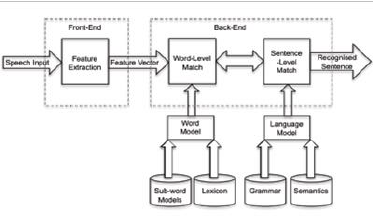
\includegraphics[width=10cm]{data_science/speech_recognition/asr_components}

Trong bước thứ nhất, trích rút thông tin \textit{Feature Extraction}, các mẫu tín hiệu được tham số hóa. Mục tiêu là trích xuất ra một tập các tham số (đặc trưng) từ tín hiệu có nhiều thông tin hữu ích nhất cho quá trình phân loại.  Các đặc trưng chính được trích xuất với điều kiện \textit{thích nghi} với các sự thay đổi của âm thanh và \textit{nhạy cảm} với các nội dung ngôn ngữ.

\definition{mô hình âm học}{Trong module phân loại, các vector đặc trưng được ánh xạ với các pattern, được gọi là \textbf{mô hình âm học} (acoustic model). Mô hình học thường là HMM được train với toàn bộ từ, hay âm như là một đơn vị ngôn ngữ.}

\definition{từ điển phát âm}{
Từ điển phát âm (pronunciation dictionary) định nghĩa cách kết hợp âm cho các ký tự. Nó có thể chứa cách phát âm khác nhau cho cùng một từ. Bảng 1 hiển thị chính xác một từ điển. Từ (graphme) ở cột bên trái ứng với cách phát âm (các âm) ở cột bên phải (các ký tự âm trong bảng được dùng phổ biến đối với tiếng Anh)
}

Ví dụ một phần của từ điển âm học tiếng Anh trong thực tế

\begin{tabular}{ | l | l | }
  \hline
  word & pronunciation \\ \hline
  INCREASE & ih n k r iy s \\ \hline
  INCREASED & ih n k r iy s t \\ \hline
  INCREASES & ih n k r iy s ah z \\ \hline
  INCREASING & ih n k r iy s ih ng  \\ \hline
  INCREASINGLY & ih n k r iy s ih ng l iy \\ \hline
  INCREDIBLE & ih n k r eh d ah b ah l \\ \hline
\end{tabular}

\definition{mô hình ngôn ngữ}{
\textit{Mô hình ngôn ngữ} (language model) chứa các thông tin về cú pháp. Mục tiêu để dự đoán khả năng một từ xuất hiện sau các từ khác trong một ngôn ngữ. Nói cách khác, xác xuất để một từ $k$ xảy ra sau khi $k-1$ từ trước đó được định nghĩa bởi $P(w_k | w_{k-1}, w_{k-2}, ..., w_1)$
}

\textbf{Mô hình hóa sub-word với HMMs}

Trong các hệ thống ASR, HMMs được dùng để biểu diễn các đơn vị dưới từ (ví dụ như âm). Với ngôn ngữ, thông thường có 40 âm. Số lượng âm phụ thuộc vào từ điển được sử dụng. Số lượng âm phụ thuộc vào từ điển được sử dụng. Mô hình từ có thể được xây dựng bằng cách kết hợp các mô hình dưới từ.

Trong thực tế, khi nhận dạng một âm phụ thuộc rất nhiều vào các âm bên cạnh. Do đó, mô hình âm phụ thuộc ngữ cảnh (*context dependence*) được sử dụng rất phổ biến. Mô hình *biphone* chú ý đến âm bên trái hoặc âm bên phải, mô hình *triphone* chú ý đến cả hai phía, với một âm, các mô hình khác nhau được sử dụng trong ngữ cảnh khác nhau. Hình dưới thể hiện các mô hình monophone, biphone và triphone của từ *bat* (b ae t)

![](http://www.igi.tugraz.at/lehre/CI/SS08/tutorials/ASR/img10.gif)

\section{Quá trình huấn luyện}

\textbf{Huấn luyện các mô hình monophone}

Một mô hình monophone là một mô hình âm học, trong đó không chứa thông tin ngữ cảnh về các âm trước và sau. Nó được sử dụng như thành phần cơ bản cho các mô hình triphone - mô hình sử dụng những thông tin về ngữ cảnh.

Việc huấn luyện sử dụng framework Gaussian Mixture Model/Hidden Markov Model.

\textbf{Dóng hàng âm thanh trong mô hình âm học}

Các tham số trong mô hình âm học được tính toán trong quá trình huấn luyện; tuy nhiên, quá trình này có thể được tối ưu hóa bởi việc lặp lại quá trình huấn luyện và dòng hàng. Còn lại là huấn luyện Viterbi (liên quan đến phương pháp này, nhưng dùng nhiều khối lượng tính toán hơn là thuật toán Forward-Backward và Expectation Maximization). Bằng cách dóng hàng âm thanh - phụ đề với mô hình âm học hiện tại, các thuật toán huấn luyện có thể sử dụng kết quả này để cải thiện và hiệu chỉnh tham số của mô hình. Do đó, mỗi quá trình huấn luyện sẽ theo bởi một bước dóng hàng trong đó âm thanh và văn bản được dóng hàng lại.

\textbf{Huấn luyện các mô hình triphone}

Trong khi các mô hình monophone đơn giản biểu diễn các đặc trưng âm thanh như một đơn âm, trong khi các âm vị sẽ thay đổi đáng kể phụ thuộc vào ngữ cảnh. Mô hình triphone thể hiện một âm trong ngữ cảnh với hai âm bên cạnh.

Đến đây, một vấn đề là không phải tất cả các đơn vị triphone được thể hiện trong dữ liệu huấn luyên. Có tất cả $\textnormal(\# of phonemes)^3$ triphone, nhưng chỉ có một tập thực sự tồn tại trong dữ liệu. Hơn nữa, các đơn vị xảy ra nhiều lần trong dữ liệu đưa ra kết quả thống kê tốt hơn trong dữ liệu. Một nhóm cây quyết định phân chia các triphones vào các nhóm, mục đích giảm thiểu tham số và đưa ra quyết định tốt hơn.

\textbf{Dóng hàng các mô hình âm học và huấn luyện lại các mô hình triphone}

Lặp lại các bước dòng hàng âm thanh và huấn luyện các mô hình triphone với các thuật toán huấn luyện để hiệu chỉnh mô hình. Các phương pháp phổ biến là delta+delta-delta, LDA-MLLT và SAT. Các giải thuật dóng hàng bao gồm dóng hàng cho từng người nói và FMLLR.

\textbf{Các thuật toán huấn luyện}

Huấn luyện delta+delta-delta tính các đặc trưng delta và double-delta, hay các hệ số động, để thêm vào các đặc trưng MFCC. Delta và delta-delta là các đặc trưng số học, tính các đạo hàm bậc 1 và 2 của tín hiệu. Do đó, phép tính toán này thường được thực hiện trên một window của các đặc trưng vector. Trong khi một window của hai đặc trưng vector có thể hiệu quả, nó là các xấp xỉ thô (giống như delta-diffrence là một xấp xỉ thô của đạo hàm). Đặc trưng delta được tính toán trong các window của các đặc trưng cơ bản, trong khi delta-delta được tính toán trong các window của đặc trựng delta.

LDA-MLLT viết tắt của Linear Discriminant Analysis - Maximum Likelihood Linear Transform. Linear Discriminant Analysis lấy các đặc trưng vector và xây dựng các trạng thái HMM, nhưng giảm thiểu không gian vector. Maximum Likelihood Linear Transfrom lấy các đặc trưng được giảm từ LDA, và thực hiện các biến đổi đối với từng người nói. MLLT sau đó thực hiện một bước chuẩn hóa, để giảm sự khác biệt giữa các người nói.

SAT viết tắt của Speaker Adaptive Training. SAT cũng thực hiện các chuẩn hóa đối với người nói bằng cách thực hiện biến đổi trên mỗi người nói. Kết quả của quá trình này đồng nhất và chuẩn hóa hơn, cho phép mô hình có thể sử dụng những tham số này để giảm thiểu sự biến đổi của âm, đối với từng người nói hoặc môi trường thu.

\textbf{Các thuật toán dóng hàng}

Thuật toán dòng hàng luôn luôn cố định, trong đó các kịch bản chấp nhận các loại đầu vào âm học khác nhau. Dòng hàng đối với từng người nói, sẽ tách biệt thông tin giữa các người nói trong quá trình dóng hàng.

fMLLR viết tắt của Feature Space Maximum Likelihood Linear Regression. Sau quá trình huấn luyện SAT, các mô hình âm học không huấn luyện trên các đặc trưng ban đầu, mà đối với các đặc trưng chuẩn hóa theo người nói. Với quá trình dóng hàng, xóa bỏ sự khác biệt giữa người nói (bằng cách nghịch đạo ma trận fMLLR), sau đó loại bỏ nó khỏi mô hình *bằng cách nhân ma trận nghịch đảo với đặc trưng vector). Mô hình âm học quasi-speaker-independent có thể sử dụng trong quá trình dóng hàng.

\textbf{Dóng hàng (Forced Alignment)}

Hệ thống nhận dạng tiếng nói sử dụng một máy tìm kiếm bên cạnh mô hình âm học và ngôn ngữ trong đó chứa tập các từ, âm và tập dữ liệu để đối chiếu với dữ liệu âm thanh cho câu nói. Máy tìm kiếm này sử dụng các đặc trưng được trích xuất bởi dữ liệu âm thanh để xác định sự xuất hiện của từ, âm và đưa ra kết quả.

![](https://www.isip.piconepress.com/projects/speech/software/tutorials/production/fundamentals/v1.0/section_04/images/srec_s04_04_p01.jpg)

Quá trình dòng hàng cũng tương tự như vậy, nhưng khác ở một điểm quan trong. Thay vì đưa vào tập các từ có thể để tìm kiếm, máy tìm kiếm đưa vào đoạn phụ đề tương ứng với câu nói. Hệ thống sau đó dóng hàng dữ liệu văn bản với dữ liệu âm thanh, xác định đoạn nào trong âm thanh tương ứng với từ cụ thể nào trong dữ liệu văn bản.

![](https://www.isip.piconepress.com/projects/speech/software/tutorials/production/fundamentals/v1.0/section_04/images/fallign_s04_04_p01.jpg)

Dóng hàng có thể sử dụng để dóng âm trong dữ liệu với bản với dữ liệu âm thanh, giống như hình dưới đây, các âm được xác định trong từng đoạn của âm thanh.

![](https://www.isip.piconepress.com/projects/speech/software/tutorials/production/fundamentals/v1.0/section_04/images/fallign2_s04_04_p01.jpg)

\section{Hidden Markov Model}

Hidden Markov Model (HMM) là mô hình trọng số với các trọng số ở cung, chỉ khả năng xuất hiện của cung.

*Một trong những ứng dụng của HMM, là phán đoán chuỗi các trạng thái thay đổi, dựa vào chuỗi các quan sát*

Các trọng số trong trạng thái gọi là observation likelihood, các trọng số ở cung gọi là transition likelihood.

Sau đây là một ví dụ:

\begin{itemize}
  \item Thời tiết trong một ngày có thể là NÓNG hoặc LẠNH
  \item Khi trời NÓNG, 20\% bạn dùng 1 viên đá, 40\% bạn dùng 2 viên, 40\% cho 3 viên.
  \item Khi trời LẠNH, 50\% bạn dùng 1 viên, 40\% bạn dùng 2, 10\% bạn dùng 3. Đây là các khả năng trong quá trình quan sát (observation likelihood)
  \item Khi trời NÓNG, 30\% nó sẽ chuyển sang LẠNH, 70\% giữ nguyên. Khi trời LẠNH, 40\% nó sẽ chuyển sang NÓNG, 60\% giữ nguyên. Đây là khả năng dịch chuyển (trainsition likelihood)
\end{itemize}

* ![https://qph.ec.quoracdn.net/main-qimg-a6744f9e17e59f3729d6fef02d54391b.webp](https://qph.ec.quoracdn.net/main-qimg-a6744f9e17e59f3729d6fef02d54391b.webp)

Giờ, giả sử chung ta quan sát trong 3 ngày, bạn dùng 1,2,3 viên đá. Thời tiết có khả năng diễn ra như thế nào?

Đến đây chúng ta dùng thuật toán Viterbi. Về cơ bản, nó là dynamic programming với hai chiều $[state, position\_in\_sequence]$

Gọi S là trạng thái hiện tại {HOT, COLD} trong quan sát i, S' là trạng thái trước đó, và A là lượng đá tiêu thụ {1, 2, 3} trong quan sát i

$$Viterbi[S,i] = Viterbi[S', i-1] * p(S|S') * p(A|S)$$
$$V[S,i] = V[S',i-1] * transition\_likelihood * observation\_likelihood$$

HMM được sử dụng trong các hệ thống thỏa mãn

\begin{enumerate}
  \item Có hữu hạn các trạng thái nội tại (internal state), là nguyên nhân của các sự kiện (external events) (các quan sát)
  \item Trạng thái nội tại không quan sát được (hidden)
  \item Trạng thái hiện tại chỉ phụ thuộc vào trạng thái trước đó (qúa trình Markov)
\end{enumerate}

Wow! George nhanh chóng liên hệ vụ của anh đấy với mô hình HMM. George nhận ra rằng CCTV footage từ các cập có thể coi như là chuỗi quan sát được, anh đấy có thể dùng mô hình và sử dụng nó để phát hiện hành vị ẩn mà Bob và William hoạt động.

\textbf{3 vấn đề cơ bản} được Jack Ferguson giới thiệu trong những năm 1960

\begin{enumerate}
  \item (Likelihood): Cho một HMM $\lambda = (A, B)$ và một chuỗi quan sát $O$, xác định likelihood $P(O|\lambda)$
  \item (Decoding): Cho một chuỗi quan sát $O$, và một HMM $\lambda = (A,B)$, xác định chuỗi ẩn $Q$ tốt nhất
  \item (Learning): Cho một chuỗi quan sát $O$, một tập các trạng thái trong HMM, học các tham số $A$ và $B$
\end{enumerate}

\section{Likelihood Computation}

Vấn đề đầu tiên là tính xác suất xảy ra của một chuỗi quan sát. Ví dụ, trong bài toán ăn đá ở hình 9.3, xác suất xảy ra chuỗi *3 1 3* là bao nhiêu?

**Tính toán Likelihood**: Chuỗi một HMM $\lambda = (A, B)$, và mỗi chuỗi quan sát $O$, xác định likelihood $P(O|\lambda)$

Thuật toán Forward, nếu sử dụng Bayes rule, để tính likelihood, cần khối lượng tính toán $N^T$ với N là số trạng thái có thể có và T là chiều dài chuỗi quan sát. Ví dụ trong bài toán gán nhãn có N=10 nhãn, chiều dài của chuỗi trung bình là 28, thì cần $10^{28}$ bước tính toán. Một giải thuật với hiệu quả $O(N^2T)$ được đề xuất với tên gọi \textbf{forward algorithm}

Tài liệu tham khảo

* http://www.igi.tugraz.at/lehre/CI/SS08/tutorials/ASR/node1.html
* https://www.isip.piconepress.com/projects/speech/software/tutorials/production/fundamentals/v1.0/section_04/s04_04_p01.html
* http://www.igi.tugraz.at/lehre/CI/SS08/tutorials/ASR/node1.html
* https://www.isip.piconepress.com/projects/speech/software/tutorials/production/fundamentals/v1.0/section_04/s04_04_p01.html
* https://www.quora.com/What-is-a-simple-explanation-of-the-Hidden-Markov-Model-algorithm

\chapter{Tổng hợp tiếng nói}

\diary{20/12/2017: Text to speech 100. Cảm ơn project rất hay của \href{https://vais.vn/vi/tai-ve/hts_for_vietnamese/}{bạn Truong Do ở vais}, nếu không có project này chắc mình phải mất rất nhiều thời gian mới có được phiên bản text to speech đầu tiên.}

Tóm lại thì việc sinh ra tiếng nói từ text gồm 4 giai đoạn

\begin{enumerate}
  \item Sinh ra features từ file wav sử dụng tool sptk
  \item Tạo một lab, trong đó có dữ liệu huấn luyện (những đặc trưng của âm thanh được trích xuất từ bước 1), text đầu vào
  \item Sử dụng htk để train dữ liệu từ thư mục lab, đầu ra là một model
  \item Sử dụng model để sinh ra output với text đầu vào, dùng hts\_engine để decode, kết quả được wav files.
\end{enumerate}

Phù. 4 bước đơn giản thế này thôi mà không biết. Lục cả internet ra mãi chẳng hiểu, cuối cùng file phân tích file `train.sh` của bạn Truong Do mới hiểu. Ahihi
%\chapter{Phân loại văn bản}

<h3>Naive Bayes Classifier</h3>
Tham khảo thư viện <a href="http://scikit-learn.org/stable/modules/naive_bayes.html" target="_blank" rel="noopener">Scikit-learn</a>

Xét bài toán classification với C classes 1,2,…,C. Tính xác suất để 1 điểm dữ liệu rơi vào class C ta có công thức: $latex P(\frac{c}{x})$. Tức tính xác suất để đầu ra là class C biết rằng đầu vào là vector x. Việc xác định class của điểm dữ liệu đó bằng cách chọn ra class có xác suất cao nhất:<p style="text-align:center;">
c = argmax($latex P(\frac{c}{x})$) với c ∈ {1,…,C}</p>
Sử dụng quy tắc Bayes:<p style="text-align:center;">
c = argmax($latex P(\frac{c}{x})$) = argmax($latex P(\frac{P(\frac{c}{x})P(x)}{P(x)}$) = argmax($latex P(\frac{P(\frac{c}{x})}{P(c)}$))</p>

<h4>Các phân phối thường dùng</h4>
<strong>Gaussian Naive Bayes</strong>
Mô hình này được sử dụng chủ yếu trong loại dữ liệu mà các thành phần là các biến liên tục.
<strong>Multinomial Naive Bayes</strong>
Mô hình này chủ yếu được sử dụng trong phân loại văn bản mà feature vectors được tính bằng Bags of Words. Lúc này, mỗi văn bản được biểu diễn bởi một vector có độ dài d chính là số từ trong từ điển. Giá trị của thành phần thứ i trong mỗi vector chính là số lần từ thứ i xuất hiện trong văn bản đó.
Khi đó, $latex P(\frac{x_i}{c})$ tỉ lệ với tần suất từ thứ i xuất hiện trong các văn bản của class c:<p style="text-align:center;"> $latex P(\frac{x_i}{c})$ = $latex \frac{Nx_i}{Nc}$</p>
<p style="padding-left:70px;">Trong đó:</p>
<p style="padding-left:90px;">$latex Nx_i$ là tổng số lần từ thứ i xuất hiện trong các văn bản của class c, nó được tính là tổng của tất cả các thành phần thứ i của các feature vectors ứng với class c.</p>
<p style="padding-left:90px;">$latex Nc$ là tổng số từ (kể cả lặp) xuất hiện trong class c. Hay bằng tổng độ dài của toàn bộ các văn bản thuộc vào class c.</p>
Nếu có một từ mới chưa bao giờ xuất hiện trong class c thì biểu thức trên sẽ bằng 0, điều này dẫn đến vế phải của c bằng 0.
<strong>Bernoulli Naive Bayes</strong>
Mô hình này được áp dụng cho các loại dữ liệu mà mỗi thành phần là một giá trị binary. Ví dụ: cũng với loại văn bản nhưng thay vì đếm tổng số lần xuất hiện của 1 từ trong văn bản, ta chỉ cần quan tâm từ đó có xuất hiện hay không.
Khi đó: $latex P(\frac{x_i}{c})$ = $latex P(\frac{i}{c})x_i$ + (1 − $latex P(\frac{i}{c})$(1 − $latex x_i $))
Với $latex P(\frac{i}{c})$ là xác suất từ thứ i xuất hiện trong các văn bản của class c.
%\chapter{Pytorch}

\diary{08/12/2017: Cảm giác \href{http://videolectures.net/deeplearning2017_chintala_torch/}{talk} của anh Soumith Chintala (Facebook, research editor) ở Deep Learning Summer School 2017 khá thú vị}

Sau khi nghe bài này thì hâm mộ luôn anh Soumith Chintala, tìm loạt bài anh trình bày luôn

* [PyTorch: Fast Differentiable Dynamic Graphs in Python with a Tensor JIT](https://www.youtube.com/watch?v=DBVLcgq2Eg0&amp;t=2s), Strange Loop Sep 2017
* [Keynote: PyTorch: Framework for fast, dynamic deep learning and scientific computing](https://www.youtube.com/watch?v=LAMwEJZqesU&amp;t=66s), EuroSciPy Aug 2017


\section{So sánh giữa Tensorflow và Pytorch?}

Có 2 điều cần phải nói khi mọi người luôn luôn so sánh giữa Tensorflow và Pytorch. (1) Tensorflow khiến mọi người "không thoải mái" (2) Pytorch thực sự là một đối thủ trên bàn cân. Một trong những câu trả lời hay nhất mình tìm được là của anh Hieu Pham (Google Brain) [trả lời trên quora (25/11/2017)](https://www.quora.com/What-are-your-reviews-between-PyTorch-and-TensorFlow/answer/Hieu-Pham-20?srid=5O2u). Điều quan trọng nhất trong câu trả lời này là *"Dùng Pytorch rất sướng cho nghiên cứu, nhưng scale lên mức business thì Tensorflow là lựa chọn tốt hơn"*

## Behind The Scene

(15/11/2017) Hôm nay bắt đầu thử nghiệm pytorch với project thần thánh classification sử dụng cnn https://github.com/Shawn1993/cnn-text-classification-pytorch

Cảm giác đầu tiên là make it run khá đơn giản

```
conda create -n test-torch python=3.5
pip install http://download.pytorch.org/whl/cu80/torch-0.2.0.post3-cp35-cp35m-manylinux1_x86_64.whl
pip install torchvision
pip install torchtext
```

Thế là `main.py` chạy! Hay thật. Còn phải vọc để bạn này chạy với CUDA nữa.

**Cài đặt CUDA trong ubuntu 16.04**

Kiểm tra VGA

```
$ lspci | grep VGA
01:00.0 VGA compatible controller: NVIDIA Corporation GM204 [GeForce GTX 980] (rev a1)
```

Kiểm tra CUDA đã cài đặt trong Ubuntu [^1]

```
$ nvcc --version
nvcc: NVIDIA (R) Cuda compiler driver
Copyright (c) 2005-2016 NVIDIA Corporation
Built on Sun_Sep__4_22:14:01_CDT_2016
Cuda compilation tools, release 8.0, V8.0.44
```

Kiểm tra pytorch chạy với cuda `test_cuda.py`

```python
import torch
print("Cuda:", torch.cuda.is_available())
```

```
$ python test_cuda.py
CUDA: True
```

Chỉ cần cài đặt thành công CUDA là pytorch tự work luôn. Ngon thật!

*Ngày X*

Chẳng hiểu sao update system kiểu nào mà hôm nay lại không sử dụng được CUDA `torch.cuda.is_available() = False`. Sau khi dùng lệnh `torch.Tensor().cuda()` thì gặp lỗi

```
AssertionError:
The NVIDIA driver on your system is too old (found version 8000).
Please update your GPU driver by downloading and installing a new
version from the URL: http://www.nvidia.com/Download/index.aspx
Alternatively, go to: https://pytorch.org/binaries to install
a PyTorch version that has been compiled with your version
of the CUDA driver.
```

Kiểm tra lại thì mình đang dùng nvidia-361, làm thử theo [link này](http://www.linuxandubuntu.com/home/how-to-install-latest-nvidia-drivers-in-linux) để update NVIDIA, chưa biết kết quả ra sao?

May quá, sau khi update lên nvida-387 là ok. Haha

**Ngày 2**

Hôm qua đã bắt đầu implement một nn với pytorch rồi. Hướng dẫn ở [Deep Learning with PyTorch: A 60 Minute Blitz](http://pytorch.org/tutorials/beginner/deep_learning_60min_blitz.html) hữu ích phết.

Hướng dẫn implement các mạng neural với pytorch rất hay tại [PyTorch-Tutorial](https://github.com/MorvanZhou/PyTorch-Tutorial)

(lượm lặt) Trang này [Awesome-pytorch-list](https://github.com/bharathgs/Awesome-pytorch-list) chứa rất nhiều link hay về pytorch như tập hợp các thư viện liên quan, các hướng dẫn và ví dụ sau đó là các cài đặt của các paper sử dụng pytorch.

(lượm lặt) Loạt video hướng dẫn pytorch [PyTorchZeroToAll](https://www.youtube.com/watch?v=SKq-pmkekTk&amp;list=PLlMkM4tgfjnJ3I-dbhO9JTw7gNty6o_2m) của tác giả Sung Kim trên youtube.

Bước tiếp theo là visualize loss và graph trong tensorboard, sử dụng [tensorboard_logger](https://github.com/TeamHG-Memex/tensorboard_logger) khá hay.

```
pip install tensorboard_logger
pip install tensorboard
```

Chạy tensorboard server

```
tensorboard --log-dir=runs
```

**Ngày 3**: Vấn đề kỹ thuật

Hôm qua cố gắng implement một phần thuật toán CNN cho bài toán phân lớp văn bản. Vấn đề đầu tiên là biểu diển sentence thế nào. Cảm giác load word vector vào khá chậm. Mà thằng tách từ của underthesea cũng chậm kinh khủng.

Một vài link tham khảo về bài toán CNN: [Implementing a CNN for Text Classification in TensorFlow](http://www.wildml.com/2015/12/implementing-a-cnn-for-text-classification-in-tensorflow/), [Text classification using CNN : Example](https://agarnitin86.github.io/blog/2016/12/23/text-classification-cnn)

[^1]: https://askubuntu.com/questions/799184/how-can-i-install-cuda-on-ubuntu-16-04


%\chapter{Big Data}

View online \href{http://magizbox.com/training/bigdata/site/}{http://magizbox.com/training/bigdata/site/}

Big Data Q&A
1. What is "Big Data"? 1
https://www.youtube.com/watch?v=TzxmjbL-i4Y

2. How big is big data? 2


3. How much data is "Big Data"? 3


4. What are characteristics of "Big Data"? 4


5. What is big data ecosystem? 5


6. What is big data landscape 6


7. What are benefits of big data? 7


https://www.youtube.com/watch?v=TzxmjbL-i4Y ↩ ↩

http://scoop.intel.com/what-happens-in-an-internet-minute/ ↩ ↩

http://www.quora.com/How-much-data-is-Big-Data ↩ ↩

https://en.wikipedia.org/wiki/Big_data#Characteristics ↩ ↩

http://www.clearpeaks.com/blog/big-data/big-data-ecosystem-spark-and-tableau ↩ ↩

https://vladimerbotsvadze.wordpress.com/2015/01/28/the-big-data-landscape-technology-businessintelligence-analytics/ ↩ ↩

http://blog.galaxyweblinks.com/big-data-with-bigger-benefits/ ↩ ↩

\section{Distribution Storage}

\subsection{HDFS}

The Hadoop Distributed File System (HDFS) — a subproject of the Apache Hadoop project—is a distributed, highly fault-tolerant file system designed to run on low-cost commodity hardware. HDFS provides high-throughput access to application data and is suitable for applications with large data sets. This article explores the primary features of HDFS and provides a high-level view of the HDFS architecture.
: sequenceiq/hadoop-docker

Big Data Stack: HDFS, Kibana, ElasticSearch, Neo4J, Apache Spark

\subsection{HBase}

Apache HBase™ is the Hadoop database, a distributed, scalable, big data store. Download Apache HBase™ Click here to download Apache HBase™.


1. When Would I Use Apache HBase? 1
HBase isn’t suitable for every problem.

First, make sure you have enough data. If you have hundreds of millions or billions of rows, then HBase is a good candidate. If you only have a few thousand/million rows, then using a traditional RDBMS might be a better choice due to the fact that all of your data might wind up on a single node (or two) and the rest of the cluster may be sitting idle.

Second, make sure you can live without all the extra features that an RDBMS provides (e.g., typed columns, secondary indexes, transactions, advanced query languages, etc.) An application built against an RDBMS cannot be "ported" to HBase by simply changing a JDBC driver, for example. Consider moving from an RDBMS to HBase as a complete redesign as opposed to a port.

Third, make sure you have enough hardware. Even HDFS doesn’t do well with anything less than 5 DataNodes (due to things such as HDFS block replication which has a default of 3), plus a NameNode.

HBase can run quite well stand-alone on a laptop - but this should be considered a development configuration only.

2. Features 2
Linear and modular scalability.
Strictly consistent reads and writes.
Automatic and configurable sharding of tables
Automatic failover support between RegionServers.
Convenient base classes for backing Hadoop MapReduce jobs with Apache HBase tables.
Easy to use Java API for client access.
Block cache and Bloom Filters for real-time queries.
Query predicate push down via server side Filters
Thrift gateway and a REST-ful Web service that supports XML, Protobuf, and binary data encoding options
Extensible jruby-based (JIRB) shell
Support for exporting metrics via the Hadoop metrics subsystem to files or Ganglia; or via JMX
3. Architecture


HBase Shell
[code lang="shell"]

list all table
list [/code]

Up & Running
1. Download
HBase 0.94.27 (HBase 0.98 won't work)

[code lang="shell"] wget https://www.apache.org/dist/hbase/hbase-0.94.27/hbase-0.94.27.tar.gz tar -xzf hbase-0.94.27.tar.gz [/code]

2. Setup
1. edit $HBASE_ROOT/conf/hbase-site.xml and add

[code lang="xml"] hbase.rootdir file:///full/path/to/where/the/data/should/be/stored hbase.cluster.distributed false [/code]

3. Verify
Go to http://localhost:60010 to see if HBase is running.

When Should I Use HBase? ↩
HBase ↩
Config HBase Remote
1. Change /etc/hosts
[code] 127.0.0.1 [username] [server_ip] hbase.io [/code]

Example

[code] 127.0.0.1 crawler 192.168.0.151 hbase.io [/code]

2. Change hostname
[code] hostname hbase.io [/code]

3. Change region servers
Edit $HBASE_ROOT/conf/regionservers

[code] hbase.io [/code]

4. Change $HABSE_ROOT/conf/hbase-site.xml
[code lang="xml" title="hbase-site.xml"] <?xml-stylesheet type="text/xsl" href="configuration.xsl"?> hbase.rootdir file:///home/username/Downloads/hbase/data hbase.cluster.distributed false hbase.zookeeper.quorum hbase.io zookeeper.znode.parent /hbase-unsecure hbase.rpc.timeout 2592000000 [/code]

Docker
HBase 0.94

Image: https://github.com/Banno/docker-hbase-standalone

[code] docker run -d -p 2181:2181 -p 60000:60000 -p 60010:60010 -p 60020:60020 -p 60030:60030 banno/hbase-standalone [/code]

Compose

[code] hbase.vmware: build: ./docker-hbase-standalone/. command: "/opt/hbase/hbase-0.94.15-cdh4.7.0/bin/hbase master start" hostname: hbase.vmware ports: - 2181:2181 - 60000:60000 - 60010:60010 - 60020:60020 - 60030:60030 volumes: - ./docker-hbase-standalone/hbase-0.94.15-cdh4.7.0:/opt/hbase/hbase-0.94.15-cdh4.7.0 - ./data/hbase:/tmp/hbase-root/hbase /code]

\section{Distribution Computing}

\subsection{Apache Spark}




Apache Spark is an open-source cluster computing framework originally developed in the AMPLab at UC Berkeley. In contrast to Hadoop's two-stage disk-based MapReduce paradigm, Spark's in-memory primitives provide performance up to 100 times faster for certain applications. By allowing user programs to load data into a cluster's memory and query it repeatedly, Spark is well-suited to machine learning algorithms.
Installation
Requirements: Hadoop, YARN

Install Hadoop

Insatll YARN

Install Java

Verification
Tutorial
From Pandas to Apache Spark’s DataFrame

Big Data Stack: HDFS, Kibana, ElasticSearch, Neo4J, Apache Spark

Apache Spark: Tutorials
Beginners Guide: Apache Spark Machine Learning with Large Data


Spark and Spark Streaming Unit Testing Recipes for Running Spark Streaming Applications in Production- Databricks

Spark Streaming


Spark and Spark Streaming Unit Testing Recipes for Running Spark Streaming Applications in Production- Databricks

\section{Components}

\subsection{Ambari}

The Apache Ambari project is aimed at making Hadoop management simpler by developing software for provisioning, managing, and monitoring Apache Hadoop clusters. Ambari provides an intuitive, easy-to-use Hadoop management web UI backed by its RESTful APIs.

Ambari enables System Administrators to:

Provision a Hadoop Cluster

Ambari provides a step-by-step wizard for installing Hadoop services across any number of hosts.
Ambari handles configuration of Hadoop services for the cluster.
Manage a Hadoop Cluster

Ambari provides central management for starting, stopping, and reconfiguring Hadoop services across the entire cluster.
Monitor a Hadoop Cluster

Ambari provides a dashboard for monitoring health and status of the Hadoop cluster.
Ambari leverages Ambari Metrics System for metrics collection.
Ambari leverages Ambari Alert Framework for system alerting and will notify you when your attention is needed (e.g., a node goes down, remaining disk space is low, etc).
Ambari enables Application Developers and System Integrators to:

Easily integrate Hadoop provisioning, management, and monitoring capabilities to their own applications with the Ambari REST APIs.
Docker


Receipts:

Image: sequenceiq/ambari (git)
Multinode cluster with Ambari 1.7.0 1
Get the docker images

[code] docker pull sequenceiq/ambari:1.7.0 [/code]

Get ambari-functions [code] curl -Lo .amb j.mp/docker-ambari-170 && . .amb [/code]

Create your cluster – automated

[code] amb-deploy-cluster 3 [/code]

Multinode cluster with Ambari 1.7.0 ↩

\subsection{Kibana}

Kibana is an open source data visualization plugin for Elasticsearch. It provides visualization capabilities on top of the content indexed on an Elasticsearch cluster. Users can create bar, line and scatter plots, or pie charts and maps on top of large volumes of data.

\subsection{Logstash}

https://www.digitalocean.com/community/tutorials/how-to-use-logstash-and-kibana-to-centralize-logs-on-centos-6

\subsection{Elasticsearch}


Elasticsearch is a search server based on Lucene. It provides a distributed, multitenant-capable full-text search engine with a RESTful web interface and schema-free JSON documents. Elasticsearch is developed in Java and is released as open source under the terms of the Apache License. Elasticsearch is the second most popular enterprise search engine
1. Basic Concenpts
Relational Database	Elasticsearch
Database	Index
Table	Type
Row	Document
Column	Field
Schema	Mapping
2. Index & Query
Get all indices
/_stats
Search API 1
Search All
/bank/_search?q=*
hits.hits – actual array of search results (defaults to first 10 documents)

Query Language
elasticsearch provides a full Query DSL based on JSON to define queries.

curl -XPOST /bank/_search
// match all, limit 10 offset 10
{
  "query": { "match_all": {} },
  "from": 10,
  "size": 10
}

// select fields
{
  "query": { "match_all": {} },
  _source: ["account_number", "balance"]
  "size": 10
}

// where account equals 20
{
  "query": { "match": { "account_number": 20 } }
}
Filter

curl -XPOST elastic:9200/index/type/_search -d '
{
  "query" : {
    "filtered" :
    {
      "query" : { "term" : { "feature" : 1 } } ,
      "filter" : {
        "and" : [
          {
            "range": {
              "_timestamp": {
                "from": 1441964671000,
                "to": 1441964672000
              }
            }
          }
        ]
      }
    }
  }
}
Sort

curl -XPOST elastic:9200/index/type/_search -d '
{
  "query" : {
    "filtered" :
    {
      "query" : { "term" : { "feature" : 1 } } ,
      "filter" : {
        "and" : [
          {
            "range": {
              "_timestamp": {
                "from": 1441964671000,
                "to": 1441964672000
              }
            }
          }
        ]
      }
    }
  }
}
3. Mapping
Timestamp 2
Enable and store timestamp

curl -XPOST localhost:9200/test
{
"mappings" : {
    "_default_":{
        "_timestamp" : {
            "enabled" : true,
            "store" : true
        }
    }
  }
}'
Relationships Management 3 4
Inner Object

👍 Easy, fast, performant
👎 No need for special queries
☛ Only applicable when one-to-one relationships are maintained
Nested

👍 Nested docs are stored in the same Lucene block as each other, which helps read/query performance. Reading a nested doc is faster than the equivalent parent/child.
👎 Updating a single field in a nested document (parent or nested children) forces ES to reindex the entire nested document. This can be very expensive for large nested docs
👎 “Cross referencing” nested documents is impossible
☛ Best suited for data that does not change frequently
Parent/Child

👍 Updating a child doc does not affect the parent or any other children, which can potentially save a lot of indexing on large docs
👎 Children are stored separately from the parent, but are routed to the same shard. So parent/children are slightly less performance on read/query than nested
👎 Parent/child mappings have a bit extra memory overhead, since ES maintains a “join” list in memory
👎 Sorting/scoring can be difficult with Parent/Child since the Has Child/Has Parent operations can be opaque at times
Denormalization

👍 You get to manage all the relations yourself!
👎 Most flexible, most administrative overhead
☛ May be more or less performant depending on your setup
4. Backup
Elastic Dump 5
Tools for moving and saving indicies.

bin/elasticdump
  --input=http://localhost:9200/index_1
  --output=http://localhost:9200/index_1_backup
  --type=data
  --scrollTime=100
Alias 6
curl -XPOST 'http://localhost:9200/_aliases' -d '
{
    &quot;actions&quot; : [
        { &quot;remove&quot; : { &quot;index&quot; : &quot;test1&quot;, &quot;alias&quot; : &quot;alias1&quot; } },
        { &quot;add&quot; : { &quot;index&quot; : &quot;test1&quot;, &quot;alias&quot; : &quot;alias2&quot; } }
    ]
}'
5. Module Scripting 7
Ranking
Rank #2 from DB-Engines Ranking of Search Engines

The Search API ↩
http://stackoverflow.com/a/17146144/772391 ↩
http://stackoverflow.com/a/23407367/772391 ↩
https://www.elastic.co/guide/en/elasticsearch/guide/current/modeling-your-data.html ↩
https://github.com/taskrabbit/elasticsearch-dump ↩
https://www.elastic.co/guide/en/elasticsearch/reference/current/indices-aliases.html ↩
https://www.elastic.co/guide/en/elasticsearch/reference/current/modules-scripting.html ↩
Elasticsearch tutorial series 1: Metric Aggregations with Social Network Data
Table of content

Avg, Max, Min, Sum Aggregation
Cardinality Aggregation
Stats Aggregation
Extended Stats Aggregation
Percentile Aggregation
Percentile Ranks Aggregation
Top hits Aggregation
Avg, Max, Min, Sum, Count Aggregation
Doc: Avg Aggregation, Doc: Max Aggregation, Doc: Min Aggregation

Get max, min, avg, sum, count about number of likes, shares, comments

Request

POST /facebook_crawler/post/_search
{"aggs":{"sum_like":{"sum":{"field":"num_like"}},"min_like":{"min":{"field":"num_like"}},"avg_like":{"avg":{"field":"num_like"}},"max_like":{"max":{"field":"num_like"}},"sum_share":{"sum":{"field":"num_share"}},"min_share":{"min":{"field":"num_share"}},"avg_share":{"avg":{"field":"num_share"}},"max_share":{"max":{"field":"num_share"}},"sum_comment":{"sum":{"field":"num_comment"}},"min_comment":{"min":{"field":"num_comment"}},"avg_comment":{"avg":{"field":"num_comment"}},"max_comment":{"max":{"field":"num_comment"}}}}
Request

{
"aggregations": {
      "avg_comment": {
         "value": 75.23860589812332
      },
      "min_like": {
         "value": 0
      },
      "avg_like": {
         "value": 1761974365266098.2
      },
      "sum_like": {
         "value": 3238508883359088600
      },
      "max_share": {
         "value": 30407
      },
      "max_comment": {
         "value": 11000
      },
      "sum_share": {
         "value": 117844
      },
      "max_like": {
         "value": 2751488761761411000
      },
      "avg_share": {
         "value": 250.19957537154988
      },
      "sum_comment": {
         "value": 28064
      },
      "min_comment": {
         "value": 2
      },
      "min_share": {
         "value": 1
      }
   }
}
Cardinality Aggregation
Cardinality Aggregation

Get total of users

Request

POST /facebook_crawler/post/_search
{
    "aggs" : {
        "num_authors" : { "cardinality" : { "field" : "from.fb_id" } }
    }
}
Response

{
   "aggregations": {
      "num_authors": {
         "value": 7385
      }
   }
}
Stats Aggregation
Doc: Stats Aggregation

Basic Stats of like, share & comment

Request

POST /facebook_crawler/post/_search
{
    "aggs" : {
        "shares" : { "stats" : { "field" : "num_share" } },
        "likes" : { "stats" : { "field" : "num_like" } },
        "comments" : { "stats" : { "field" : "num_comment" } }
    }
}
Response

{
   "aggregations": {
      "shares": {
         "count": 471,
         "min": 1,
         "max": 30407,
         "avg": 250.19957537154988,
         "sum": 117844
      },
      "comments": {
         "count": 373,
         "min": 2,
         "max": 11000,
         "avg": 75.23860589812332,
         "sum": 28064
      },
      "likes": {
         "count": 1838,
         "min": 0,
         "max": 2751488761761411000,
         "avg": 1761974365266098.2,
         "sum": 3238508883359088600
      }
   }
}
Extended Stats Aggregation
Extended Stats Aggregation

Stats of like, share & comment with more metrics, such as sum, std_deviation, std_deviation_bounds, variance

Request

POST /facebook_crawler/post/_search
{
    "aggs" : {
        "like_stats" : { "extended_stats" : { "field" : "num_like" } },
        "share_stats" : { "extended_stats" : { "field" : "num_share" } },
        "comment_stats" : { "extended_stats" : { "field" : "num_comment" } }
    }
}
Response

{
   "aggregations": {
      "like_stats": {
         "count": 1838,
         "min": 0,
         "max": 2751488761761411000,
         "avg": 1761974365266098.2,
         "sum": 3238508883359088600,
         "sum_of_squares": 7.667542671405507e+36,
         "variance": 4.168572634260795e+33,
         "std_deviation": 64564484310345070,
         "std_deviation_bounds": {
            "upper": 130890942985956240,
            "lower": -127366994255424050
         }
      },
      "share_stats": {
         "count": 471,
         "min": 1,
         "max": 30407,
         "avg": 250.19957537154988,
         "sum": 117844,
         "sum_of_squares": 1769467022,
         "variance": 3694230.367812983,
         "std_deviation": 1922.0380765773043,
         "std_deviation_bounds": {
            "upper": 4094.2757285261587,
            "lower": -3593.8765777830586
         }
      },
      "comment_stats": {
         "count": 373,
         "min": 2,
         "max": 11000,
         "avg": 75.23860589812332,
         "sum": 28064,
         "sum_of_squares": 131531392,
         "variance": 346970.2299304962,
         "std_deviation": 589.0417896299856,
         "std_deviation_bounds": {
            "upper": 1253.3221851580945,
            "lower": -1102.844973361848
         }
      }
   }
}
Percentiles Aggregation
Doc: Percentiles Aggregation

Comment, Like, Share Percentiles

Request

POST /facebook_crawler/post/_search
{"aggs":{"like_percentiles":{"percentiles":{"field":"num_like"}},"share_percentiles":{"percentiles":{"field":"num_share"}},"comment_percentiles":{"percentiles":{"field":"num_comment"}}}}
Response

{
"aggregations": {
      "like_percentiles": {
         "values": {
            "1.0": 0,
            "5.0": 0,
            "25.0": 4,
            "50.0": 18.35,
            "75.0": 72.53579545454545,
            "95.0": 71343.74999999999,
            "99.0": 4338260523723.276
         }
      },
      "comment_percentiles": {
         "values": {
            "1.0": 2,
            "5.0": 2,
            "25.0": 5,
            "50.0": 10,
            "75.0": 26,
            "95.0": 139.39999999999998,
            "99.0": 1000
         }
      },
      "share_percentiles": {
         "values": {
            "1.0": 1,
            "5.0": 1,
            "25.0": 1,
            "50.0": 4,
            "75.0": 25,
            "95.0": 251.5,
            "99.0": 5560.3
         }
      }
   }
}
Like Percentiles with custom percents

Request

POST /facebook_crawler/post/_search
{
   "aggs": {
      "share_percentiles": {
         "percentiles": {
            "field": "num_share",
            "percents": [0, 10, 80, 90, 95]
         }
      }
   }
}
Response

{
   "aggregations": {
      "share_percentiles": {
         "values": {
            "0.0": 1,
            "10.0": 1,
            "80.0": 37.33333333333333,
            "90.0": 97,
            "95.0": 251.5
         }
      }
   }
}
Percentile Ranks Aggregation
Doc: Percentile Ranks Aggregation

How like, share, comment distribute

Request

POST /facebook_crawler/post/_search
{
   "aggs": {
      "like_percentile_ranks": {
         "percentile_ranks": {
            "field": "num_like",
            "values": [10, 100, 1000, 10000, 1000000, 10000000]
         }
      },
      "share_percentile_ranks": {
         "percentile_ranks": {
            "field": "num_share",
            "values": [10, 100, 1000, 10000, 1000000, 10000000]
         }
      },
      "comment_percentile_ranks": {
         "percentile_ranks": {
            "field": "num_comment",
            "values": [10, 100, 1000, 10000, 1000000, 10000000]
         }
      }
   }
}
Response

{
   "aggregations": {
      "share_percentile_ranks": {
         "values": {
            "10.0": 60.438782731776364,
            "100.0": 89.91507430997878,
            "1000.0": 97.37406386327386,
            "10000.0": 99.31579836222765,
            "1000000.0": 100,
            "1.0E7": 100
         }
      },
      "like_percentile_ranks": {
         "values": {
            "10.0": 39.281828073993466,
            "100.0": 79.39530545624125,
            "1000.0": 90.98349676683587,
            "10000.0": 94.14527905373414,
            "1000000.0": 95.9014681663581,
            "1.0E7": 96.57661015941164
         }
      },
      "comment_percentile_ranks": {
         "values": {
            "10.0": 49.865951742627345,
            "100.0": 92.18395545473294,
            "1000.0": 98.92761394101876,
            "10000.0": 99.56773202397807,
            "1000000.0": 100,
            "1.0E7": 100
         }
      }
   }
}
As we can see, only 0.7% posts have more than 10k shares, onley 0.04% posts have more than 10k comment, but there is an odd here. 4.1% posts have more than 1M like (WHAT!!!). We can spot some strange here.

Top hits Aggregation
Doc: Top hits Aggregation

Example

Request

Response

{

An Aggregation
Doc: Link

Config
elasticsearch.yml

discovery.zen.minimum_master_nodes: 1
discovery.zen.ping.multicast.enabled: false
discovery.zen.ping.unicast.hosts: ["localhost"]

network.host: 0.0.0.0
http.cors.enabled: true
http.cors.allow-origin: '*'
script.inline: on
script.indexed: on
Docker
Image

https://hub.docker.com/r/_/elasticsearch/

Run

docker run -d -v "$PWD/esdata":/usr/share/elasticsearch/data elasticsearch
Docker Folder

elasticsearch/
├── config
│   └── elasticsearch.yml
└── Dockerfile
Dockerfile

FROM elasticsearch:2.2.0

ADD config/elasticsearch.yml /elasticsearch/config/elasticsearch.yml
Compose

elasticsearch:
    build: ./elasticsearch/.
    ports:
       - 9200:9200
       - 9300:9300
    volumes:
       - ./data/elasticsearch:/usr/share/elasticsearch/data
Elasticsearch: Search Ignore Accents
The ICU 1 2 analysis plug-in for Elasticsearch uses the International Components for Unicode (ICU) libraries to provide a rich set of tools for dealing with Unicode. These include the icu_tokenizer, which is particularly useful for Asian languages, and a number of token filters that are essential for correct matching and sorting in all languages other than English.

Step 1: Install ICU-Plugin 3
cd /usr/share/elasticsearch
sudo bin/plugin install analysis-icu
Step 2: Create an analyzer setting:
"settings": {
      "analysis": {
         "analyzer": {
            "vnanalysis": {
               "tokenizer": "icu_tokenizer",
               "filter": [
                  "icu_folding",
                  "icu_normalizer"
               ]
            }
         }
      }
   }
Step 3: Create your index, create a field with type string and analyzer is vnanalysis you have created
"key": {
     "type": "string",
     "analyzer": "vnanalysis"
}
Step 4: Search with sense
POST /your_index/your_doc_type/_search
{
   "query": {
      "match": {
         "key": "kiem tra"
      }
   }
}
ES: Import CSV to Elasticsearch
https://gist.github.com/clemsos/8668698

Install lastest Elasticdump with NVM
As a matter of best practice we’ll update our packages:

apt-get update
The build-essential package should already be installed, however, we’re going still going to include it in our command for installation:

apt-get install build-essential libssl-dev
To install or update nvm, you can use the install script using cURL:

curl -o- https://raw.githubusercontent.com/creationix/nvm/v0.31.0/install.sh | bash
if you have below problem or after you type nvm ls-remote command it result N/A: curl: (77) error setting certificate verify locations: CAfile: /etc/pki/tls/certs/ca-bundle.crt CApath: none

head to this 1:

or Wget:

wget -qO- https://raw.githubusercontent.com/creationix/nvm/v0.31.0/install.sh | bash
Don't forget to restart your terminal

Then you use the following command to list available versions of nodejs

nvm ls-remote
To download, compile, and install the latest v5.0.x release of node, do this:

nvm install 5.0
And then in any new shell just use the installed version:

nvm use 5.0
Or you can just run it:

nvm run 5.0 --version
Or, you can run any arbitrary command in a subshell with the desired version of node:

nvm exec 4.2 node --version
You can also get the path to the executable to where it was installed:

nvm which 5.0
Node Version Manager

how to solve https problem ↩

ICU plug-in Github ↩

Installing the ICU plug-in ↩

\subsection{Neo4J}

version: 2.3.1

Neo4j is an open-source graph database, implemented in Java. The developers describe Neo4j as "embedded, disk-based, fully transactional Java persistence engine that stores data structured in graphs rather than in tables". Neo4j is the most popular graph database.

Installation

Docker
Docker Image: https://hub.docker.com/r/library/neo4j/

Run these below command to open neo4j

# clone datahub project
git clone https://github.com/magizbox/datahub.git

# change folder to datahub directory
cd datahub

# set your config in docker-compose.yml

# run docker
docker-compose up

Cypher

Schema Discovery
List all nodes label, list all relation type

> START n=node(*) RETURN distinct labels(n)

> match n-[r]-() return distinct type(r)
UI Way: Click to Overtab in Neo4j Browser

Sample 10 entities
> MATCH (n:Entity) RETURN n, rand() as random ORDER BY random LIMIT 10
Group By
http://www.markhneedham.com/blog/2013/02/17/neo4jcypher-sql-style-group-by-functionality/

Graph Algorithms

shortestPath, dijkstra

POST http://localhost:7474/db/data/node/72/paths

Headers
Accept: application/json
Authorization: Basic bmVvNGo6cGFzc3dk

Body
{
  "to" : "http://localhost:7474/db/data/node/77",
  "max_depth" : 5,
  "relationships" : {
    "type" : "FRIEND",
    "direction" : "out"
  },
  "algorithm" : "shortestPath"
}
Graph Analystic

pagerank, closeness_centrality, betweenness_centrality, triangle_count, connected_components, strongly_connected_components

Client

In this article you will know how to connect to neo4j database from python.

Python Client
We can use Py2neo to connect to neo4j from python.

Py2neo is a client library and comprehensive toolkit for working with Neo4j from within Python applications and from the command line. The core library has no external dependencies and has been carefully designed to be easy and intuitive to use.

Snippets to connect, create, add nodes, add relationship and update property

from py2neo import authenticate, Graph, Node, Relationship
# connect to graph
authenticate("localhost:7474", "neo4j", "passwd")
graph = Graph("http://localhost:7474/db/data/")

# create unique
graph.schema.create_uniqueness_constraint('Person', 'name')

# add nodes
graph.create(Node.cast('Person', {"name": "Alice"}))
graph.create(Node.cast('Person', {"name": "Bob"}))

# add relationship
source = graph.merge_one("Person", "name", "Alice")
target = graph.merge_one("Person", "name", "Bob")
graph.create_unique(Relationship(source, "FRIEND", target))

# update property
alice = graph.merge_one("Person", "name", "Alice")
alice["age"] = 30
alice.push()

\section{Web Crawling}

\subsection{Introduction}

Web Crawler
Static Crawler

Apache Nutch
Dynamic Crawler

nutch-selenium
Intelligent Extractor

boilerpipe
Web Content Extraction Through Machine Learning
Priority Crawler, Social Crawler

Features a crawler must provide
We list the desiderata for web crawlers in two categories: features that web crawlers must provide, followed by features they should provide.

Robustness:

The Web contains servers that create spider traps, which are generators of web pages that mislead crawlers into getting stuck fetching an infinite number of pages in a particular domain. Crawlers must be designed to be resilient to such traps. Not all such traps are malicious; some are the inadvertent side-effect of faulty website development.

Politeness:

Web servers have both implicit and explicit policies regulating the rate at which a crawler can visit them. These politeness policies must be respected.

Features a crawler should provide
Distributed The crawler should have the ability to execute in a distributed fashion across multiple machines.

Scalable

The crawler architecture should permit scaling up the crawl rate by adding extra machines and bandwidth.

Performance and efficiency

The crawl system should make efficient use of various system resources including processor, storage and network bandwidth.

Quality

Given that a significant fraction of all web pages are of poor utility for serving user query needs, the crawler should be biased towards fetching ``useful'' pages first.

Freshness

In many applications, the crawler should operate in continuous mode: it should obtain fresh copies of previously fetched pages. A search engine crawler, for instance, can thus ensure that the search engine's index contains a fairly current representation of each indexed web page. For such continuous crawling, a crawler should be able to crawl a page with a frequency that approximates the rate of change of that page.

Extensible

Crawlers should be designed to be extensible in many ways - to cope with new data formats, new fetch protocols, and so on. This demands that the crawler architecture be modular.

Crawling
The basic operation of any hypertext crawler (whether for the Web, an intranet or other hypertext document collection) is as follows.

The crawler begins with one or more URLs that constitute a seed set. It picks a URL from this seed set, then fetches the web page at that URL.
The fetched page is then parsed, to extract both the text and the links from the page (each of which points to another URL).
The extracted text is fed to a text indexer.
The extracted links (URLs) are then added to a URL frontier, which at all times consists of URLs whose corresponding pages have yet to be fetched by the crawler.
Initially, the URL frontier contains the seed set; as pages are fetched, the corresponding URLs are deleted from the URL frontier. The entire process may be viewed as traversing the web graph. In continuous crawling, the URL of a fetched page is added back to the frontier for fetching again in the future.
This seemingly simple recursive traversal of the web graph is complicated by the many demands on a practical web crawling system: the crawler has to be distributed, scalable, efficient, polite, robust and extensible while fetching pages of high quality. We examine the effects of each of these issues. Our treatment follows the design of the Mercator crawler that has formed the basis of a number of research and commercial crawlers. As a reference point, fetching a billion pages (a small fraction of the static Web at present) in a month-long crawl requires fetching several hundred pages each second. We will see how to use a multi-threaded design to address several bottlenecks in the overall crawler system in order to attain this fetch rate.

Before proceeding to this detailed description, we reiterate for readers who may attempt to build crawlers of some basic properties any non-professional crawler should satisfy:

Only one connection should be open to any given host at a time.
A waiting time of a few seconds should occur between successive requests to a host.
Politeness restrictions should be obeyed.

A New Approach to Dynamic Crawler
Build a crawler system for dynamic websites is not easy task. While you can use a web browser automator (like selenium), or event when you can integrate selenium with nutch (by using nutch-selenium). These solutions are still hard to develop, hard to test and hard to manage sessions because we still "translate" our process to languages (such as java or python)

I suppose a new approach for this problem. Instead of using a web browser automator, we can inject native javascript codes into browser (via extension or add-on).The advantages of this approach is we can easily inject third party libraries (like jquery (for dom selector), Run.js (for complicated process) and APIs that supported by browsers). And we can take advance of debugging tool and testing framework in javascript world.

If you want to know about more details, feel free to contact me.

\subsection{Scrapy}

Scrapy
An open source and collaborative framework for extracting the data you need from websites. In a fast, simple, yet extensible way.

Build and run your web spiders
$ pip install scrapy
$ cat > myspider.py <<EOF
import scrapy

class BlogSpider(scrapy.Spider):
    name = 'blogspider'
    start_urls = ['https://blog.scrapinghub.com']

    def parse(self, response):
        for title in response.css('h2.entry-title'):
            yield {'title': title.css('a ::text').extract_first()}

        next_page = response.css('div.prev-post > a ::attr(href)').extract_first()
        if next_page:
            yield scrapy.Request(response.urljoin(next_page), callback=self.parse)
EOF
$ scrapy runspider myspider.py
Deploy them to Scrapy Cloud
$ shub login
Insert your Scrapinghub API Key: <API_KEY>

# Deploy the spider to Scrapy Cloud

$ shub deploy

# Schedule the spider for execution
 shub schedule blogspider
Spider blogspider scheduled, watch it running here:
https://app.scrapinghub.com/p/26731/job/1/8

# Retrieve the scraped data
$ shub items 26731/1/8
{"title": "Improved Frontera: Web Crawling at Scale with Python 3 Support"}
{"title": "How to Crawl the Web Politely with Scrapy"}
...

\subsection{Apache Nutch}

Highly extensible, highly scalable Web crawler 1 Nutch is a well matured, production ready Web crawler. Nutch 1.x enables fine grained configuration, relying on Apache Hadoop™ data structures, which are great for batch processing.

History


Usecases


1. Features 1
1. Transparency Nutch is open source, so anyone can see how the ranking algorithms work. With commercial search engines, the precise details of the algorithms are secret so you can never know why a particular search result is ranked as it is. Furthermore, some search engines allow rankings to be based on payments, rather than on the relevance of the site's contents. Nutch is a good fit for academic and government organizations, where the perception of fairness of rankings may be more important.

2. Understanding We don't have the source code to Google, so Nutch is probably the best we have. It's interesting to see how a large search engine works. Nutch has been built using ideas from academia and industry: for instance, core parts of Nutch are currently being re-implemented to use the MapReduce.

Map Reduce distributed processing model, which emerged from Google Labs last year. And Nutch is attractive for researchers who want to try out new search algorithms, since it is so easy to extend.

3. Extensibility Don't like the way other search engines display their results? Write your own search engine--using Nutch! Nutch is very flexible: it can be customized and incorporated into your application. For developers, Nutch is a great platform for adding search to heterogeneous collections of information, and being able to customize the search interface, or extend the out-of-the-box functionality through the plugin mechanism. For example, you can integrate it into your site to add a search capability.

Process 5
0. initialize CrawlDb, inject seed URLs Repeat generate-fetch-update cycle n times:

1. The Injector takes all the URLs of the nutch.txt file and adds them to the CrawlDB. As a central part of Nutch, the CrawlDB maintains information on all known URLs (fetch schedule, fetch status, metadata, …).

2. Based on the data of CrawlDB, the Generator creates a fetchlist and places it in a newly created Segment directory.

3. Next, the Fetcher gets the content of the URLs on the fetchlist and writes it back to the Segment directory. This step usually is the most time-consuming one.

4. Now the Parser processes the content of each web page and for example omits all html tags. If the crawl functions as an update or an extension to an already existing one (e.g. depth of 3), the Updater would add the new data to the CrawlDB as a next step.

5. Before indexing, all the links need to be inverted by Link Inverter, which takes into account that not the number of outgoing links of a web page is of interest, but rather the number of inbound links. This is quite similar to how Google PageRank works and is important for the scoring function. The inverted links are saved in the Linkdb.

6-7. Using data from all possible sources (CrawlDB, LinkDB and Segments), the Indexer creates an index and saves it within the Solr directory. For indexing, the popular Lucene library is used. Now, the user can search for information regarding the crawled web pages via Solr.

Installation
Requirements

1. OpenJDK 7

2. Nutch 2.3 RC (yes, you need 2.3, 2.2 will not work)

wget https://archive.apache.org/dist/nutch/2.3/apache-nutch-2.3-src.tar.gz
tar -xzf apache-nutch-2.3-src.tar.gz
3. HBase 0.94.27 (HBase 0.98 won't work)

wget https://www.apache.org/dist/hbase/hbase-0.94.27/hbase-0.94.27.tar.gz
tar -xzf hbase-0.94.27.tar.gz
4. ElasticSearch 1.7

wget https://download.elastic.co/elasticsearch/elasticsearch/elasticsearch-1.7.0.tar.gz
tar -xzf elasticsearch-1.7.0.tar.gz
Other Options: nutch-2.3, hbase-0.94.26, ElasticSearch 1.4

Setup HBase
1. edit $HBASE_ROOT/conf/hbase-site.xml and add

<configuration>
    <property>
        <name>hbase.rootdir</name>
        <value>file:///full/path/to/where/the/data/should/be/stored</value>
    </property>
    <property>
        <name>hbase.cluster.distributed</name>
        <value>false</value>
    </property>
</configuration>
2. edit $HBASE_ROOT/conf/hbase-env.sh and enable JAVA_HOME and set it to the proper path:

-# export JAVA_HOME=/usr/java/jdk1.6.0/
+export JAVA_HOME=/usr/lib/jvm/java-7-openjdk-amd64/
This step might seem redundant, but even with JAVA_HOME being set in my shell, HBase just didn't recognize it.

3. kick off HBase:

$ $HBASE_ROOT/bin/start-hbase.sh
Configure Nutch
1. Enable the HBase dependency in $NUTCH_ROOT/ivy/ivy.xml by uncommenting the line

<dependency org="org.apache.gora" name="gora-hbase" rev="0.5" conf="*->default" />
2. Configure the HBase adapter by editing the $NUTCH_ROOT/conf/gora.properties

-#gora.datastore.default=org.apache.gora.mock.store.MockDataStore
+gora.datastore.default=org.apache.gora.hbase.store.HBaseStore
3. Build Nutch

$ cd $NUTCH_ROOT && ant clean && ant runtime
This can take a while and creates $NUTCH_ROOT/runtime/local.

4. configure Nutch by editing $NUTCH_ROOT/runtime/local/conf/nutch-site.xml

<configuration>
    <property>
        <name>http.agent.name</name>
        <value>mycrawlername</value>
        <!-- this can be changed to something more sane if you like -->
    </property>
    <property>
        <name>http.robots.agents</name>
        <value>mycrawlername</value>
        <!-- this is the robot name we're looking for in robots.txt files -->
    </property>
    <property>
        <name>storage.data.store.class</name>
        <value>org.apache.gora.hbase.store.HBaseStore</value>
    </property>
    <property>
        <name>plugin.includes</name>
        <!-- do \*\*NOT\*\* enable the parse-html plugin, if you want proper HTML parsing. Use something like parse-tika! -->
        <value>
            protocol-httpclient|urlfilter-regex|parse-(text|tika|js)|index-(basic|anchor)|query-(basic|site|url)|response-(json|xml)|summary-basic|scoring-opic|urlnormalizer-(pass|regex|basic)|indexer-elastic
        </value>
    </property>
    <property>
        <name>db.ignore.external.links</name>
        <value>true</value>
        <!-- do not leave the seeded domains (optional) -->
    </property>
    <property>
        <name>elastic.host</name>
        <value>localhost</value>
        <!-- where is ElasticSearch listening -->
    </property>
</configuration>
or you configure Nutch by editing $NUTCH_ROOT/runtime/local/conf/nutch-site.xml

<configuration>
    <property>
        <name>plugin.includes</name>
        <!-- do \*\*NOT\*\* enable the parse-html plugin, if you want proper HTML parsing. Use something like parse-tika! -->
        <value>
            protocol-http|protocol-httpclient|urlfilter-regex|
parse-(text|tika|js)|index-(basic|anchor)|query-(basic|site|url)|response-(json|xml)|
summary-basic|scoring-opic|urlnormalizer-(pass|regex|basic)|indexer-elastic|
index-metadata|index-more
        </value>
    </property>
    <property>
        <name>db.ignore.external.links</name>
        <value>true</value>
        <!-- do not leave the seeded domains (optional) -->
    </property>


<!-- elasticsearch index properties -->
<property>
  <name>elastic.host</name>
  <value>localhost</value>
  <description>The hostname to send documents to using TransportClient.
  Either host and port must be defined or cluster.
  </description>
</property>

<property>
  <name>elastic.port</name>
  <value>9300</value>
  <description>
  The port to connect to using TransportClient.
  </description>
</property>
<property>
  <name>elastic.index</name>
  <value>nutch</value>
  <description>
  The name of the elasticsearch index. Will normally be autocreated if it
  doesn't exist.
  </description>
</property>
<!-- end index -->
</configuration>
5. configure HBase integration by editing $NUTCH_ROOT/runtime/local/conf/hbase-site.xml

<?xml version="1.0" encoding="UTF-8"?>
<configuration>
   <property>
      <name>hbase.rootdir</name>
      <value>file:///full/path/to/where/the/data/should/be/stored</value>
      <!-- same path as you've given for HBase above -->
   </property>
   <property>
      <name>hbase.cluster.distributed</name>
      <value>false</value>
   </property>
</configuration>
or you configure HBase integration by editing $NUTCH_ROOT/runtime/local/conf/hbase-site.xml:

<configuration>
  <property>
    <name>hbase.rootdir</name>
    <value>file:///$PATH/database</value>
  </property>
  <property>
    <name>hbase.cluster.distributed</name>
    <value>false</value>
  </property>
  <property>
    <name>hbase.zookeeper.quorum</name>
    <value>hbase.io</value>
  </property>
  <property>
    <name>zookeeper.znode.parent</name>
    <value>/hbase-unsecure</value>
  </property>
  <property>
    <name>hbase.rpc.timeout</name>
    <value>2592000000</value>
  </property>
</configuration>
That's it. Everything is now setup to crawl websites.

Run Nutch
1. Create an empty directory. Add a textfile containing a list of seed URLs

$ mkdir seed
$ echo "https://www.website.com" >> seed/urls.txt
$ echo "https://www.another.com" >> seed/urls.txt
$ echo "https://www.example.com" >> seed/urls.txt
Inject them into Nutch by giving a file URL (!)

$ $NUTCH_ROOT/runtime/local/bin/nutch inject file:///path/to/seed/
2. Generate a new set of URLs to fetch.

This is is based on both the injected URLs as well as outdated URLs in the Nutch crawl db.

$ $NUTCH_ROOT/runtime/local/bin/nutch generate -topN 10
The above command will create job batches for 10 URLs.

3. Fetch the URLs. We are not clustering, so we can simply fetch all batches:

$ $NUTCH_ROOT/runtime/local/bin/nutch fetch -all
4. Now we parse all fetched pages:

$ $NUTCH_ROOT/runtime/local/bin/nutch parse -all
5. Last step: Update Nutch's internal database:

$ $NUTCH_ROOT/runtime/local/bin/nutch updatedb -all
On the first run, this will only crawl the injected URLs. The procedure above is supposed to be repeated regulargy to keep the index up to date.

6. Putting Documents into ElasticSearch

$ $NUTCH_ROOT/runtime/local/bin/nutch index -all
Configuration
Crawl nutch via proxy

Change $NUTCH_ROOT/runtime/local/conf/nutch-site.xml

<configuration>
    <property>
        <name>http.proxy.host</name>
        <value>192.168.80.1</value>
        <description>The proxy hostname. If empty, no proxy is used.</description>
    </property>
    <property>
        <name>http.proxy.port</name>
        <value>port</value>
        <description>The proxy port.</description>
    </property>
    <property>
        <name>http.proxy.username</name>
        <value>username</value>
        <description>Username for proxy. This will be used by 'protocol-httpclient', if the proxy server requests basic,
            digest
            and/or NTLM authentication. To use this, 'protocol-httpclient' must be present in the value of
            'plugin.includes'
            property. NOTE: For NTLM authentication, do not prefix the username with the domain, i.e. 'susam' is correct
            whereas
            'DOMAINsusam' is incorrect.
        </description>
    </property>
    <property>
        <name>http.proxy.password</name>
        <value>password</value>
        <description>Password for proxy. This will be used by 'protocol-httpclient', if the proxy server requests basic,
            digest
            and/or NTLM authentication. To use this, 'protocol-httpclient' must be present in the value of
            'plugin.includes'
            property.
        </description>
    </property>
</configuration>
Nutch Plugins
Extension Points
In writing a plugin, you're actually providing one or more extensions of the existing extension-points . The core Nutch extension-points are themselves defined in a plugin, the NutchExtensionPoints plugin (they are listed in the NutchExtensionPoints plugin.xml file). Each extension-point defines an interface that must be implemented by the extension. The core extension points are:

Point	Description	Example
IndexWriter	Writes crawled data to a specific indexing backends (Solr, ElasticSearch, a CVS file, etc.).
IndexingFilter	Permits one to add metadata to the indexed fields. All plugins found which implement this extension point are run sequentially on the parse (from javadoc).
Parser	Parser implementations read through fetched documents in order to extract data to be indexed. This is what you need to implement if you want Nutch to be able to parse a new type of content, or extract more data from currently parseable content.
HtmlParseFilter	Permits one to add additional metadata to HTML parses (from javadoc).
Protocol	Protocol implementations allow Nutch to use different protocols (ftp, http, etc.) to fetch documents.
URLFilter	URLFilter implementations limit the URLs that Nutch attempts to fetch. The RegexURLFilter distributed with Nutch provides a great deal of control over what URLs Nutch crawls, however if you have very complicated rules about what URLs you want to crawl, you can write your own implementation.
URLNormalizer	Interface used to convert URLs to normal form and optionally perform substitutions.
ScoringFilter	A contract defining behavior of scoring plugins. A scoring filter will manipulate scoring variables in CrawlDatum and in resulting search indexes. Filters can be chained in a specific order, to provide multi-stage scoring adjustments.
SegmentMergeFilter	Interface used to filter segments during segment merge. It allows filtering on more sophisticated criteria than just URLs. In particular it allows filtering based on metadata collected while parsing page.
Getting Nutch to Use a Plugin
In order to get Nutch to use a given plugin, you need to edit your conf/nutch-site.xml file and add the name of the plugin to the list of plugin.includes. Additionally we are required to add the various build configurations to build.xml in the plugin directory.

Develop nutch plugins
Project structure of a plugin
plugin-name
  plugin.xml
  build.xml
  ivy.xml
  src
    org
      apache
        nutch
          indexer
            uml-meta # source folder
              URLMetaIndexingFilter.java
          scoring
            uml-meta # source folder
              URLMetaScoringFilter.java
  test
    org
      apache
        nutch
          indexer
            uml-meta # test folder
              URLMetaIndexingFilterTest.java
          scoring
            uml-meta # test folder
              URLMetaScoringFilterTest.java
Follow this link to read develop nutch plugins

\subsubsection{Architecture}

Architectures


Data Structure
The web database is a specialized persistent data structure for mirroring the structure and properties of the web graph being crawled. It persists as long as the web graph that is being crawled (and re-crawled) exists, which may be months or years. The WebDB is used only by the crawler and does not play any role during searching. The WebDB stores two types of entities: pages and links.

A page represents a page on the Web, and is indexed by its URL and the MD5 hash of its contents. Other pertinent information is stored, too, including

the number of links in the page (also called outlinks);
fetch information (such as when the page is due to be refetched);
the page's score, which is a measure of how important the page is (for example, one measure of importance awards high scores to pages that are linked to from many other pages).
A link represents a link from one web page (the source) to another (the target). In the WebDB web graph, the nodes are pages and the edges are links.

A segment is a collection of pages fetched and indexed by the crawler in a single run. The fetchlist for a segment is a list of URLs for the crawler to fetch, and is generated from the WebDB. The fetcher output is the data retrieved from the pages in the fetchlist. The fetcher output for the segment is indexed and the index is stored in the segment. Any given segment has a limited lifespan, since it is obsolete as soon as all of its pages have been re-crawled. The default re-fetch interval is 30 days, so it is usually a good idea to delete segments older than this, particularly as they take up so much disk space. Segments are named by the date and time they were created, so it's easy to tell how old they are.

The index is the inverted index of all of the pages the system has retrieved, and is created by merging all of the individual segment indexes. Nutch uses Lucene for its indexing, so all of the Lucene tools and APIs are available to interact with the generated index. Since this has the potential to cause confusion, it is worth mentioning that the Lucene index format has a concept of segments, too, and these are different from Nutch segments. A Lucene segment is a portion of a Lucene index, whereas a Nutch segment is a fetched and indexed portion of the WebDB.

View gora-hbase-mapping.xml for more details

\subsubsection{Config}

Config nutch run intellij
Copy file

copy all the files in the runtime/conf on out/test/apache-Nutch-2.3 and out/production/apache-Nutch-2.3

add these lines to file $NUTCH_SRC/out/test/nutch-site.xml

<property>
   <name>plugin.folders</name>
   <value><nutch_src>/build/plugins</value>
 </property>
Run nutch in intellij
Run->Edit Configurations...->add path agrs:path to file list links crawler
Dev Nutch in Intellij
Receipts: IntellIJ 14, Apache Nutch 2.3

1. Get Nutch source

wget http://www.eu.apache.org/dist/nutch/2.3/apache-nutch-2.3-src.tar.gz
tar -xzf apache-nutch-2.3-src.tar.gz
2. Import Nutch source in IntellIJ

[wonderplugin_slider id="1"]

3. Get Dependencies by Ant

[wonderplugin_slider id="3"]

4. Import Dependencies to IntellIJ

[wonderplugin_slider id="4"]

Nutch Dev
1.Intasll java in ubuntu

-Downloads java version .zip

 http://www.oracle.com/technetwork/java/javase/downloads/jdk7-downloads-1880260.html
-Create folder jvm

 sudo mkdir /usr/lib/jvm/
-Cd to folder downloads java version .zip

 sudo mv jdk1.7.0_x/ /usr/lib/jvm/jdk1.7.0_x
-Run command line

  sudo update-alternatives --install /usr/bin/java java /usr/lib/jvm/jdk1.7.0_x/jre/bin/java 0
-Tets version java

  java -version
2.Intasll ant in ubuntu

-Downloads ant

http://ant.apache.org/manualdownload.cgi
-Add path ant vao file environment

 sudo nano /etc/environment
 $ANT_ROOT/bin
-Run command line

source /etc/environment
ant -version
3.Intasll hbase in ubuntu

-Downloads and extract hbase 0.94.27

  https://archive.apache.org/dist/hbase/hbase-0.94.27/
-Edit file $HABSE_ROOT/conf/hbase-site.xml

 <configuration>
  <property>
    <name>hbase.rootdir</name>
    <value>file:///$PATH_DATA_BASE/database</value>
  </property>
  <property>
    <name>hbase.cluster.distributed</name>
    <value>false</value>
  </property>
  <property>
    <name>hbase.zookeeper.quorum</name>
    <value>hbase.io</value>
  </property>
  <property>
    <name>zookeeper.znode.parent</name>
    <value>/hbase-unsecure</value>
  </property>
  <property>
    <name>hbase.rpc.timeout</name>
    <value>2592000000</value>
  </property>
</configuration>
-Edit file $HBASE_ROOT/conf/hbase-env.sh

  export JAVA_HOME=$PATH_JAVA_HOME
-Edit file $HBASE_ROOT/conf/regionservers

hbase.io.nutch
-Edit file hosts in ubuntu

  sudo nano /etc/hosts
  {ip} hbase.io.nutch
-Edit file hostname in ubuntu

 sudo nano /etc/hostname
 hbase.io.nutch
-Run and stop hbase in ubuntu

 Run hbase : cd $HBASE_ROOT/bin ./start-hbase.sh
 Stop hbase: cd $HBASE_ROOT/bin ./stop-hbase.sh
*Error in intasll hbase

- Error regionserver localhost(Edit file hosts and file host name)
- Error client no remote server intasll hbase(Turn off file firewall)
4.Build nutch in ant

-Downloads and extract nutch

  http://nutch.apache.org/
-Edit file $NUTCH_ROOT/ivy/ivy.xml

 <dependency org="org.apache.gora" name="gora-hbase" rev="0.5"
conf="*->default" />
-Edit file $NUTCH_ROOT/ivy/ivysettings.xml

 #<property name="repo.maven.org"
 #   value="http://repo1.maven.org/maven2/"
 #  override="false"/>

<property name = "repo.maven.org"
   value = "http://maven.oschina.net/content/groups/public/"
   override = "false" />
-Edit file $NUTCH_ROOT/conf/nutch-site.xml

<configuration>
<property>
   <name>plugin.folders</name>
   <value>$NUTCH_ROOT/build/plugins</value>
 </property>
<property>
        <name>http.agent.name</name>
        <value>mycrawlername</value>
        <!-- this can be changed to something more sane if you like -->
    </property>
    <property>
        <name>http.robots.agents</name>
        <value>mycrawlername</value>
        <!-- this is the robot name we're looking for in robots.txt files -->
    </property>
    <property>
        <name>storage.data.store.class</name>
        <value>org.apache.gora.hbase.store.HBaseStore</value>
    </property>
    <property>
        <name>plugin.includes</name>
        <!-- do \*\*NOT\*\* enable the parse-html plugin, if you want proper HTML parsing. Use something like parse-tika! -->
        <value>
            protocol-http|protocol-httpclient|urlfilter-regex|parse-(text|tika|js)|index-(basic|anchor)|query-(basic|site|url)|response-(json|xml)|summary-basic|scoring-opic|urlnormalizer-(pass|regex|basic)|indexer-elastic|index-metadata|index-more
        </value>
    </property>
    <property>
        <name>db.ignore.external.links</name>
        <value>true</value>
        <!-- do not leave the seeded domains (optional) -->
    </property>


<!-- elasticsearch index properties -->
<property>
  <name>elastic.host</name>
  <value>localhost</value>
  <description>The hostname to send documents to using TransportClient.
  Either host and port must be defined or cluster.
  </description>
</property>

<property>
  <name>elastic.port</name>
  <value>9300</value>
  <description>
  The port to connect to using TransportClient.
  </description>
</property>
<property>
  <name>elastic.index</name>
  <value>nutch</value>
  <description>
  The name of the elasticsearch index. Will normally be autocreated if it
  doesn't exist.
  </description>
</property>
<!-- end index -->

<property>
        <name>http.proxy.host</name>
        <value>192.168.80.1</value>
    </property>
    <property>
        <name>http.proxy.port</name>
        <value>8080</value>
    </property>
    <property>
        <name>http.proxy.username</name>
        <value>user1</value>
    </property>
    <property>
        <name>http.proxy.password</name>
        <value>user1</value>
    </property>
</configuration>
-Edit file file $NUTCH_ROOT/conf/gora.property

 gora.datastore.default=org.apache.gora.hbase.store.HBaseStore
-Build nucth

 ant runtime
 or
 ant eclipse -verbose
-Create file links

-Run nutch

 cd $NUTCH_ROOT/runtime/local/bin
 run inject : ./nutch inject file:///$PATH_LIKNS
 run generate : ./nutch generate -topN 10
 run fetch : ./nutch fetch -all
 run parse : ./nutch parse -all
 run updatedb : ./nutch updatedb -all
-Downloads and extract elastic

 https://www.elastic.co/downloads/elasticsearch
-Run elastic

cd $ELASTIC/bin
./elasticsearch
-Index data in elastic

 cd $NUTCH_ROOT/runtime/bin
 run index : ./nutch index -all
5.Run nutch intellij

Change $NUTCH_ROOT/runtime/local/conf/hbase-site.xml

<configuration>
<property>
<name>hbase.rootdir</name>
<value>file:///home/hainv/Downloads/crawler/data</value>
</property>
<property>
<name>hbase.cluster.distributed</name>
<value>false</value>
</property>
<property>
<name>hbase.zookeeper.quorum</name>
<value>hbase.io</value>
</property>
<property>
<name>zookeeper.znode.parent</name>
<value>/hbase-unsecure</value>
</property>
<property>
<name>hbase.rpc.timeout</name>
<value>2592000000</value>
</property>
</configuration>
Nutch plugin intellij
1.Structure nutch :[1]
2.Run nutch intellij
Downloads nucth2.3:http://nutch.apache.org/downloads.html Editing file $NUTCH_ROOT/ivy/ivysettings.xml

<ivysettings>
  <property name="oss.sonatype.org"
    value="http://oss.sonatype.org/content/repositories/releases/"
    override="false"/>
  <property name = "repo.maven.org"
      value = "http://maven.oschina.net/content/groups/public/"
      override = "false" />
  <property name="repository.apache.org"
    value="https://repository.apache.org/content/repositories/snapshots/"
    override="false"/>
  <property name="maven2.pattern"
    value="[organisation]/[module]/[revision]/[module]-[revision]"/>
  <property name="maven2.pattern.ext"
    value="${maven2.pattern}.[ext]"/>
  <!-- pull in the local repository -->
  <include url="${ivy.default.conf.dir}/ivyconf-local.xml"/>
  <settings defaultResolver="default"/>
  <resolvers>
    <ibiblio name="maven2"
      root="${repo.maven.org}"
      pattern="${maven2.pattern.ext}"
      m2compatible="true"
      />
    <ibiblio name="apache-snapshot"
      root="${repository.apache.org}"
      changingPattern=".*-SNAPSHOT"
      m2compatible="true"
      />
    <ibiblio name="restlet"
      root="http://maven.restlet.org"
      pattern="${maven2.pattern.ext}"
      m2compatible="true"
      />
     <ibiblio name="sonatype"
      root="${oss.sonatype.org}"
      pattern="${maven2.pattern.ext}"
      m2compatible="true"
      />

    <chain name="default" dual="true">
      <resolver ref="local"/>
      <resolver ref="maven2"/>
      <resolver ref="sonatype"/>
      <resolver ref="apache-snapshot"/>
    </chain>
    <chain name="internal">
      <resolver ref="local"/>
    </chain>
    <chain name="external">
      <resolver ref="maven2"/>
      <resolver ref="sonatype"/>
    </chain>
    <chain name="external-and-snapshots">
      <resolver ref="maven2"/>
      <resolver ref="apache-snapshot"/>
      <resolver ref="sonatype"/>
    </chain>
    <chain name="restletchain">
      <resolver ref="restlet"/>
    </chain>
  </resolvers>
  <modules>
    <module organisation="org.apache.nutch" name=".*" resolver="internal"/>
    <module organisation="org.restlet" name=".*" resolver="restletchain"/>
    <module organisation="org.restlet.jse" name=".*" resolver="restletchain"/>
  </modules>
</ivysettings>
Editing file $NUTCH_ROOT/ivy/ivy.xml

<dependency org="org.apache.gora" name="gora-hbase" rev="0.5" conf="*->default" />
Editing file $NUCTH_ROOT/conf/gora.properties

gora.datastore.default=org.apache.gora.hbase.store.HBaseStore
Editing file $NUTCH_ROOT/conf/nutch_site.xml

<configuration>
<property>
   <name>plugin.folders</name>
   <value>$NUTCH_ROOT/build/plugins</value>
 </property>
<property>
        <name>http.agent.name</name>
        <value>mycrawlername</value>
        <!-- this can be changed to something more sane if you like -->
    </property>
    <property>
        <name>http.robots.agents</name>
        <value>mycrawlername</value>
        <!-- this is the robot name we're looking for in robots.txt files -->
    </property>
    <property>
        <name>storage.data.store.class</name>
        <value>org.apache.gora.hbase.store.HBaseStore</value>
    </property>
    <property>
        <name>plugin.includes</name>
        <!-- do \*\*NOT\*\* enable the parse-html plugin, if you want proper HTML parsing. Use something like parse-tika! -->
        <value>
            protocol-httpclient|urlfilter-regex|parse-(text|tika|js)|index-(basic|anchor)|query-(basic|site|url)|response-(json|xml)|summary-basic|scoring-opic|urlnormalizer-(pass|regex|basic)|indexer-elastic
        </value>
    </property>
    <property>
        <name>db.ignore.external.links</name>
        <value>true</value>
        <!-- do not leave the seeded domains (optional) -->
    </property>
    <property>
        <name>elastic.host</name>
        <value>localhost</value>
        <!-- where is ElasticSearch listening -->
    </property>

<property>
        <name>http.proxy.host</name>
        <value>192.168.80.1</value>
        <description>The proxy hostname. If empty, no proxy is used.</description>
    </property>
    <property>
        <name>http.proxy.port</name>
        <value>8080</value>
        <description>The proxy port.</description>
    </property>
    <property>
        <name>http.proxy.username</name>
        <value>user1</value>
        <description>Username for proxy. This will be used by 'protocol-httpclient', if the proxy server requests basic,
            digest
            and/or NTLM authentication. To use this, 'protocol-httpclient' must be present in the value of
            'plugin.includes'
            property. NOTE: For NTLM authentication, do not prefix the username with the domain, i.e. 'susam' is correct
            whereas
            'DOMAINsusam' is incorrect.
        </description>
    </property>
    <property>
        <name>http.proxy.password</name>
        <value>user1</value>
        <description>Password for proxy. This will be used by 'protocol-httpclient', if the proxy server requests basic,
            digest
            and/or NTLM authentication. To use this, 'protocol-httpclient' must be present in the value of
            'plugin.includes'
            property.
        </description>
    </property>
</configuration>
Editing file $NUCTH_ROOT/conf/hbase-site.xml

<configuration>
    <property>
        <name>hbase.rootdir</name>
        <value>file:///home/rombk/Downloads/database</value>
    </property>
    <property>
        <name>hbase.cluster.distributed</name>
        <value>false</value>
    </property>
    <property>
        <name>hbase.zookeeper.quorum</name>
        <value>hbase.io</value>
    </property>
    <property>
        <name>zookeeper.znode.parent</name>
        <value>/hbase-unsecure</value>
    </property>
    <property>
        <name>hbase.rpc.timeout</name>
        <value>2592000000</value>
    </property>
</configuration>
Run terminal

 ant eclipse -verbose
Import nucth intellij


3.Run plugin creativecommons
Sample plugins that parse and index Creative Commons medadata.1 Step 1. Create folder creativecommons in path $NUTCH_HOME/out/test/

Step 2. Create file nutch-site.xml in folder $NUTCH_HOME/out/test/creativecommons and add content

<?xml version="1.0"?>
<?xml-stylesheet type="text/xsl" href="configuration.xsl"?>
<!-- Put site-specific property overrides in this file. -->
<configuration>
<property>
   <name>plugin.folders</name>
   <value>$NUTCH_HOME/build/plugins</value>
 </property>
<property>
   <name>http.agent.name</name>
   <value>mycrawlername</value>
<!-- this can be changed to something more sane if you like -->
</property>
<property>
   <name>http.robots.agents</name>
   <value>mycrawlername</value>
<!-- this is the robot name we're looking for in robots.txt files -->
</property>
<property>
   <name>storage.data.store.class</name>
   <value>org.apache.gora.hbase.store.HBaseStore</value>
</property>
<property>
   <name>plugin.includes</name>
  <!-- do \*\*NOT\*\* enable the parse-html plugin, if you want proper HTML parsing. Use something like parse-tika! -->
  <value>indexer-elastic|creativecommons|parse-html</value>
</property>
<property>
   <name>db.ignore.external.links</name>
   <value>true</value>
<!-- do not leave the seeded domains (optional) -->
</property>
<property>
   <name>elastic.host</name>
   <value>localhost</value>
<!-- where is ElasticSearch listening -->
</property>
<!-- config proxy-->
<property>
   <name>http.proxy.host</name>
   <value><hosts></value>
   <description>The proxy hostname. If empty, no proxy is used.</description>
</property>
<property>
   <name>http.proxy.port</name>
   <value><port></value>
   <description>The proxy port.</description>
</property>
<property>
   <name>http.proxy.username</name>
   <value><user1></value>
   <description>Username for proxy. This will be used by 'protocol-httpclient', if the proxy server requests basic,
digest
and/or NTLM authentication. To use this, 'protocol-httpclient' must be present in the value of
'plugin.includes'
property. NOTE: For NTLM authentication, do not prefix the username with the domain, i.e. 'susam' is correct
whereas
'DOMAINsusam' is incorrect.
     </description>
</property>
<property>
   <name>http.proxy.password</name>
   <value><user1></value>
   <description>Password for proxy. This will be used by 'protocol-httpclient', if the proxy server requests basic,
digest
and/or NTLM authentication. To use this, 'protocol-httpclient' must be present in the value of
'plugin.includes'
property.
    </description>
</property>
</configuration>
2.Run plugin feed
Plugin feed parsing of rss Error : Parsing of RSS feeds fails (tejasp) [2] and read file $NUTCH_ROOT/CHANFES.txt


  \part{Linh tinh}

\chapter{Nghiên cứu}

\diary{01/11/2017 Không biết mình có phải làm nghiên cứu không nữa? Vừa kiêm phát triển, vừa đọc paper mỗi ngày. Thôi, cứ (miễn cưỡng) cho là nghiên cứu viên đi.}

\section{Các công cụ}

\subsection{Google Scholar \& Semantic Scholar}

\href{https://scholar.google.com.vn/}{Google Scholar} vẫn là lựa chọn tốt

\begin{itemize}
  \item Tìm kiếm tác giả theo lĩnh vực nghiên cứu và quốc gia: sử dụng filter label: + đuôi
    \begin{itemize}
      \item ví dụ: \href{https://scholar.google.com.vn/citations?hl=en&amp;view_op=search_authors&amp;mauthors=label\%3Anatural_language_processing+.vn&amp;btnG=}{danh sách các nhà nghiên cứu Việt Nam thuộc lĩnh vực xử lý ngôn ngữ tự nhiên}
    \end{itemize}
  \item danh sách này đã sắp xếp theo lượng trích dẫn
\end{itemize}


Bên cạnh đó còn có \href{https://www.semanticscholar.org/}{semanticscholar} (một project của \href{http://allenai.org/}{allenai}) với các killer features

\begin{itemize}
  \item \href{https://www.semanticscholar.org/search?venue\%5B\%5D=ACL&amp;q=sentiment&amp;sort=relevance}{Tìm kiếm các bài báo khoa học với từ khóa và filter theo năm, tên hội nghị}
  \item \href{https://www.semanticscholar.org/author/Christopher-D-Manning/1812612}{Xem những người ảnh hưởng, ảnh hưởng bởi một nhà nghiên cứu, cũng như xem co-author, journals và conferences mà một nhà nghiên cứu hay gửi bài}
\end{itemize}

\subsection{Mendeley}

Mendeley rất tốt cho việc quản lý và lưu trữ. Tuy nhiên điểm hạn chế lại là không lưu thông tin về citation

\subsection{Hội nghị và tạp chí}

Các hội nghị tốt về xử lý ngôn ngữ tự nhiên

\begin{itemize}
  \item Rank A: ACL, EACL, NAACL, EMNLP, CoNLL
  \item Rank B: SemEval
\end{itemize}

Các tạp chí

\begin{itemize}
  \item \href{http://www.mitpressjournals.org/loi/coli}{Computational Linguistics (CL)}
\end{itemize}

\subsection{Câu chuyện của Scihub}

Sci-Hub được tạo ra vào ngày 5 tháng 9 năm 2011, do nhà nghiên cứu đến từ Kazakhstan, \href{https://en.wikipedia.org/wiki/Alexandra_Elbakyan}{Alexandra Elbakyan}

Hãy nghe chia sẻ của cô về sự ra đời của Sci-Hub

> Khi tôi còn là một sinh viên tại Đại học Kazakhstan, tôi không có quyền truy cập vào bất kỳ tài liệu nghiên cứu. Những bài báo tôi cần cho dự án nghiên cứu của tôi. Thanh toán 32 USD thì thật là điên rồ khi bạn cần phải đọc lướt hoặc đọc hàng chục hoặc hàng trăm tờ để làm nghiên cứu. Tôi có được những bài báo nhờ vào trộm chúng. Sau đó tôi thấy có rất nhiều và rất nhiều nhà nghiên cứu (thậm chí không phải sinh viên, nhưng các nhà nghiên cứu trường đại học) giống như tôi, đặc biệt là ở các nước đang phát triển. Họ đã tạo ra các cộng đồng trực tuyến (diễn đàn) để giải quyết vấn đề này. Tôi là một thành viên tích cực trong một cộng đồng như vậy ở Nga. Ở đây ai cần có một bài nghiên cứu, nhưng không thể trả tiền cho nó, có thể đặt một yêu cầu và các thành viên khác, những người có thể có được những giấy sẽ gửi nó cho miễn phí qua email. Tôi có thể lấy bất cứ bài nào, vì vậy tôi đã giải quyết nhiều yêu cầu và người ta luôn rất biết ơn sự giúp đỡ của tôi. Sau đó, tôi tạo Sci-Hub.org, một trang web mà chỉ đơn giản là làm cho quá trình này tự động và các trang web ngay lập tức đã trở thành phổ biến.

Về phần mình, là một nhà nghiên cứu trẻ, đương nhiên phải đọc liên tục. Các báo cáo ở Việt Nam về xử lý ngôn ngữ tự nhiên thì thường không tải lên các trang mở như arxiv.org, các kỷ yếu hội nghị cũng không public các proceedings. Thật sự scihub đã giúp mình rất nhiều.

\textbf{Scihub bị chặn}

Vào thời điểm này (12/2017), scihub bị chặn quyết liệt. Hóng được trên page facebook của scihub các cách truy cập scihub. Đã thử các domain khác như .tw, .hk. Mọi chuyện vẫn ổn cho đến hôm nay (21/12/2017), không thể truy cập vào nữa.

Đành phải cài tor để truy cập vào scihub ở địa chỉ \href{http://scihub22266oqcxt.onion/https://dl.acm.org/citation.cfm?id=1852627}{http://scihub22266oqcxt.onion}. Và mọi chuyện lại ổn.

\section{Làm sao để nghiên cứu tốt}

\begin{itemize}
  \item Làm việc mỗi ngày
  \item Cập nhật các kết quả từ các hội nghị, tạp chí
  \item Viết nhật ký nghiên cứu mỗi tuần (tổng kết công việc tuần trước, các ý tưởng mới, kế hoạch tuần này)
\end{itemize}

\section{Sách giáo khoa}

\href{https://gallery.mailchimp.com/dc3a7ef4d750c0abfc19202a3/files/Machine_Learning_Yearning_V0.5_01.pdf}{Machine Learning Yearning, by Andrew Ng}

\section{Lượm lặt}

\href{https://www.kdnuggets.com/2017/10/3-popular-courses-deep-learning.html}{Review các khóa học Deep Learning}

\section{Thuyết trình}

Tự nhiên hôm nay (22/01/2018) lại đọc được bài \href{https://huynq.net/you-suck-at-powerpoint/}{You suck at PowerPoint}, thấy hay quá.

Sau đây là 10 lỗi thường gặp khi làm bài thuyết trình

\begin{enumerate}
  \item Quá nhiều chữ trong 1 slide.
  \item Màu chữ và màu nền không tương phản với nhau.
  \item Dùng clip art, word art.
  \item Hình ảnh sử dụng trong slide chất lượng kém, scale sai tỉ lệ.
  \item Sử dụng nhiều font chữ trong 1 slide.
  \item Lạm dụng quá nhiều hiệu ứng (animation/transition).
  \item Bài presentation không có cấu trúc.
  \item Slide không ăn nhập gì với nội dung trình bày.
  \item Không ghi rõ nguồn khi sử dụng tài liệu, hình ảnh của người khác.
  \item Ý thức của người làm slide
\end{enumerate}

\chapter{Nghề lập trình}

Chân kinh con đường lập trình: [Teach Yourself Programming in Ten Years. Peter Norvig](http://norvig.com/21-days.html)

Trang web hữu ích

* Chia sẻ thú vị: [15 năm lập trình ở Việt Nam](https://vozforums.com/showthread.php?t=3431312) của Blanic (vozfourm)
* Trang web chứa cheatsheet so sánh các ngôn ngữ lập trình và công nghệ [http://hyperpolyglot.org/](http://hyperpolyglot.org/)

### 01/11/2017

Vậy là đã vào nghề (đi làm full time trả lương) được 3 năm rưỡi rồi. Thời gian trôi qua nhanh như *ó chạy ngoài đồng thật. Tâm đắc nhất với câu trong một quyển gì đó của anh lead HR google. Có 4 level của nghề nghiệp. 1 là thỏa mãn được yêu cầu cả bản. 2 là dự đoán được tương lai. 3 là cá nhân hóa (ý nói là tận tình với các khách hàng). 4 là phiêu diêu tự tại. Hay thật! Bao giờ mới được vào mức 4 đây.
\chapter{Latex}

15/12/2017:

Hôm nay tự nhiên nổi hứng vẽ hình trên latex. Thấy blog này là một guide line khá tốt về viết blog phần mềm. Quyết định cài latex

Theo [hướng dẫn này](http://milq.github.io/install-latex-ubuntu-debian/)

```
sudo apt-get install texlive-full
sudo apt-get install texmaker
```

Tìm được ngay bên này https://www.overleaf.com/ có vẻ rất hay luôn

Hướng dẫn cực kì cơ bản http://www.math.uni-leipzig.de/~hellmund/LaTeX/pgf-tut.pdf

Chương trình đầu tiên, vẽ diagram cho LanguageFlow

\begin{lstlisting}[language=text]
\documentclass[border=10pt]{standalone}
\usepackage{verbatim}
\begin{comment}
\end{comment}
\usepackage{tikz}
\begin{document}
\begin{tikzpicture}
    \node[draw] (model) at (0, 0) {Model Folder};
    \node[draw] (analyze) at (6, 0) {Analyze Folder};
    \node[draw] (board) at (3,2) {Board};
    \node[draw] (logger) at (3, -2) {Logger};

    \path[->, densely dotted] (board.east)
    	edge [out=0, in=90]
    	node[fill=white, pos=.5] {\tiny (1) init}
        (analyze.north) ;
    \path[->, densely dotted] (board.south)
    	edge [out=-90, in=180]
    	node[fill=white, pos=.3] {\tiny (2) serve}
        (analyze.west) ;
	\path[->, densely dotted] (logger.west)
    	edge [out=180, in=-90]
    	node[fill=white, pos=.7] {\tiny (1) read}
        (model.south) ;
	\path[->, densely dotted] (logger.east)
    	edge [out=0, in=-90]
    	node[fill=white, pos=.7] {\tiny (2) write}
        (analyze.south) ;
\end{tikzpicture}
\end{document}
\end{lstlisting}

Doc! Doc! Doc! https://en.wikibooks.org/wiki/LaTeX/PGF/TikZ
\chapter{Chào hàng}

**16/01/2018** Bố khỉ. Hôm nay gửi lời mời kết bạn đến một thằng làm research về speech mà nó "chửi" mình không biết pitch. Tổ sư. Tuy nhiên, nó cũng dạy mình một bài học hay về pitch.

Chửi nó là vậy nhưng lần sau sẽ phải đầu tư nhiều hơn cho các lời pitch.

Vẫn không ưa Huyền Chíp như ngày nào, nhưng [bài này](https://www.facebook.com/notes/huyen-chip/k%E1%BB%B9-n%C4%83ng-ch%C3%A0o-h%C3%A0ng-pitch/1337740609675643/) cũng đáng đọc.

Tóm lại skill này có 4 phần

1. Ngôn ngữ không trau chuốt
2. Giới thiệu bản thân không tốt
3. Không chỉ ra cho người nhận rằng họ sẽ được gì
4. Không có phương án hành động

Đối với email, thì cần triển khai thế này

* [Chào hỏi]
* [Giới thiệu bản thân một cách nào đó để người đọc quan tâm đến bạn]
* [Giải thích lý do bạn biết đến người này và bạn ấn tượng thế nào với họ -- ai cũng thích được nghe khen]
* [Bạn muốn gì từ người đó và họ sẽ được gì từ việc này]
* [Kết thúc]
\chapter{Phát triển phần mềm}

* Phát triển phần mềm là một việc đau khổ. Từ việc quản lý code và version, packing, documentation. Dưới đây là lượm lặt những nguyên tắc cơ bản của mình.

### Quản lý phiên bản

Việc đánh số phiên bản các thay đổi của phần mềm khi có hàm được thêm, lỗi được sửa, hay các phiên bản tiền phát hành cần thống nhất theo chuẩn của [semversion]. Điều này giúp nhóm có thể tương tác dễ hơn với người dùng cuối.

![](https://raw.githubusercontent.com/magizbox/magizbox/master/wordpress/phat_trien_phan_mem/version.png)

**Đánh số phiên bản**

Phiên bản được đánh theo chuẩn của [semversion](https://semver.org/).

* Mỗi khi một bug được sửa, phiên bản sẽ tăng lên một patch
* Mỗi khi có một hàm mới được thêm, phiên bản sẽ tăng lên một patch.
* Khi một phiên bản mới được phát hành, phiên bản sẽ tăng lên một minor.
* Trước khi phát hành, bắt đầu với x.y.z-rc, x.y.z-rc.1, x.y.z-rc.2. Cuối cùng mới là x.y.z
* Mỗi khi phiên bản rc lỗi, khi public lại, đặt phiên bản alpha x.y.z-alpha.t (một phương án tốt hơn là cài đặt thông qua github)

**Đánh số phiên bản trên git**

Ở nhánh develop, mỗi lần merge sẽ được đánh version theo PATCH, thể hiện một bug được sửa hoặc một thay đổi của hàm

Ở nhánh master, mỗi lần release sẽ được thêm các chỉ như x.y1.0-rc, x.y1.0-rc.1, x.y1.0-rc, x.y1.0

*Vẫn còn lăn tăn*:

* Hiện tại theo workflow này thì chưa cần sử dụng alpha, beta (chắc là khi đó đã có lượt người sử dụng mới cần đến những phiên bản như thế này)

**Tải phần mềm lên pypi**

Làm theo hướng dẫn [tại đây](http://peterdowns.com/posts/first-time-with-pypi.html)

1. Cấu hình file `.pypirc`
2. Upload lên pypi

```
python setup.py sdist upload -r pypi
```
\chapter{Phương pháp làm việc}

Xây dựng phương pháp làm việc là một điều không đơn giản. Với kinh nghiệm 3 năm làm việc, trải qua 2 project. Mà vẫn chưa produce được sản phẩm cho khách hàng. Thiết nghĩ mình nên viết phương pháp làm việc ra để xem xét lại. Có lẽ sẽ có ích cho mọi người.

Làm sao để làm việc hiệu quả, hay xây dựng phương pháp làm việc hữu ích? Câu trả lời ngắn gọn là "Một công cụ không bao giờ đủ".

<!--more-->

### Nội dung

1. [Làm sao để đánh giá công việc trong khoảng thời gian dài hạn?](#section1)
2. [Làm sao để quản lý project?](#section2)
3. [Làm sao để công việc trôi chảy?](#section3)
4. [Làm sao để xem xét lại quá trình làm việc?](#section4)

<p id="section1">&nbsp;</p>

### Làm sao để đánh giá công việc trong khoảng thời gian dài hạn?

Câu trả lời OKR (Objectives and Key Results)

![](https://image.slidesharecdn.com/20170829-ale2017-okr-170829060043/95/agile-leadership-and-goal-management-with-objectives-key-results-okrs-ale-2017-prague-23-638.jpg?cb=1503986541)
*OKR Framework*

Đầu mỗi quý ⏱, nên dành vài ngày cho việc xây dựng mục tiêu và những kết quả quan trọng cho quý tới. Cũng như review lại ☕ kết quả quý trước.

Bước 1: Xây dựng mục tiêu cá nhân (Objectives)

Bước 2: Xây dựng các Key Results cho mục tiêu này

Bước 3: Lên kế hoạch để hiện thực hóa các Key Results

<p id="section2">&nbsp;</p>

### Làm sao để quản lý một project

Meistertask

![](https://focus.meisterlabs.com/wp-content/uploads/2015/03/Projectboard_MT_EN-1.png)
*Meister Task*

<p id="section3">&nbsp;</p>

### Làm sao để công việc trôi chảy?

Có vẻ trello là công cụ thích hợp

Bước 1: Tạo một team với một cái tên thật ấn tượng (của mình là Strong Coder)

Trong phần Description của team, nên viết Objectives and Key Results của quý này

Sau đây là một ví dụ

```
Objectives and Key Results

-> Build Vietnamese Sentiment Analysis
-> Develop underthesea
-> Deep Learning Book
```

Bước 2: Đầu mỗi tuần, tạo một board với tên là thời gian ứng với tuần đó (của mình là `2017 | Fight 02 (11/12 - 16/12)`)

Board này sẽ gồm 5 mục: "TODO", "PROGRESSING", "Early Fight", "Late Fight", "HABBIT", được lấy cảm hứng từ Kanban Board

![](https://mktgcdn.leankit.com/uploads/images/general/_xLarge/kanban_guide_print_KPO_bleed_board2.jpg)
*Trello Board example*

* ⏱ Mỗi khi không có việc gì làm, xem xét card trong "TODO"
* ⏱ [FOCUS] tập trung làm việc trong "PROGRESSING"
* ☕ Xem xét lại thói quen làm việc với "HABBIT"

Một Card cho Trello cần có

* Tên công việc (title)
* Độ quan trọng (thể hiện ở label xanh (chưa quan trọng), vàng (bình thường), đỏ (quan trọng))
* Hạn chót của công việc (due date)

Sắp xếp TODO theo thứ tự độ quan trọng và Due date

<p id="section4">&nbsp;</p>

### Làm sao để xem xét lại quá trình làm việc?

Nhật lý làm việc hàng tuần ☕. Việc này lên được thực hiện vào đầu tuần ⏱. Có 3 nội dung quan trọng trong nhật ký làm việc (ngoài gió mây trăng cảm xúc, quan hệ với đồng nghiệp...)

* Kết quả công việc tuần này
* Những công việc chưa làm? Lý do tại sao chưa hoàn thành?
* Dự định cho tuần tới

*Đang nghiên cứu*

**Làm sao để lưu lại các ý tưởng, công việc cần làm?**: Dùng chức năng checklist của card trong meister. Khi có ý tưởng mới, sẽ thêm một mục trong checklist

**Làm sao để tập trung vào công việc quan trọng?**: Dùng chức năng tag của meister, mỗi một công việc sẽ được đánh sao (với các mức 5 sao, 3 sao, 1 sao), thể hiện mức độ quan trọng của công việc. Mỗi một sprint nên chỉ tập trung vào 10 star, một product backlog chỉ nên có 30 star.

**Tài liệu của dự án**: Sử dụng Google Drive, tài liệu mô tả dự án sẽ được link vào card tương ứng trong meister.
  \bibliography{mybib}{}
  \bibliographystyle{ksfh_nat}
  \addcontentsline{toc}{part}{Tài liệu}
%  \addcontentsline{toc}{part}{\refname}
  \printindex
  \addcontentsline{toc}{part}{Chỉ mục}
\end{document}